%================================================================
% SLO
%----------------------------------------------------------------
% datoteka: 	thesis_template.tex
%
% opis: 		predloga za pisanje diplomskega dela v formatu LaTeX na
% 				Univerza v Ljubljani, Fakulteti za računalništvo in informatiko
%
% pripravili: 	Matej Kristan, Zoran Bosnić, Andrej Čopar,
%			  	po začetni predlogi Gašperja Fijavža
%
% popravil: 	Domen Rački, Jaka Cikač, Matej Kristan
%
% verzija: 		30. september 2016 (dodan razširjeni povzetek)
%================================================================


%================================================================
% SLO: definiraj strukturo dokumenta
% ENG: define file structure
%================================================================
\documentclass[a4paper, 12pt]{book}
 

%================================================================
% SLO: Odkomentiraj "\SLOtrue " za izbiro slovenskega jezika
% ENG: Uncomment "\SLOfalse" to chose English languagge
%================================================================
\newif\ifSLO
\newif\ifTRACKEXIST
\newif\ifTRACKCS
\newif\ifPROGRAMMM
\newif\ifPROGRAMEMAI


% ---------------------------------------------------------------------------------------
% IMPORTANT: Adjust the thesis language, your study program and track within this block
% ---------------------------------------------------------------------------------------
% ** switch language ** %
\SLOtrue % Enables Slovenian language
%\SLOfalse  % Enables English language

% ** Switch programs: ** %

% ** Uncomment if Program: Computer Science, Track: Computer Science **%
\TRACKCStrue
\TRACKEXISTtrue

% ** Uncomment if Program: Computer Science, Track: Data Science **%
%\TRACKCSfalse
%\TRACKEXISTtrue

% ** Uncomment if Program: Multimedia **%
%\PROGRAMMMtrue 
%\TRACKEXISTfalse 

% ** Uncomment if Program: EMAI **%
%\PROGRAMEMAItrue
%\SLOfalse 

% -------------------------------------------------------------------------------------------
% End of language, program and track adjustment
% -------------------------------------------------------------------------------------------


%================================================================
% SLO: vključi oblikovanje in pakete
% ENG: include design and packages
%================================================================
%----------------------------------------------------------------
% SLO: LaTeX paketi
% ENG: LateX packages
%----------------------------------------------------------------
% SLO: omogoča uporabo slovenskih (latinskih) črk kodiranih v formatu UTF-8
% ENG: enables the use of slovene (latin) caracters encoded in the UFT-8 format
\usepackage[utf8x]{inputenc}
%\inputencoding{utf8}
% SLO: naloži, med drugim, slovenske delilne vzorce
% ENG: loads, among others, slovene dividing patterns
\usepackage[slovene,english]{babel}
% SLO: poskrbi za postavitev strani
% ENG: takes care of the page layout
\usepackage{fancyhdr}
% SLO: za vlaganje slik različnih formatov
% ENG: for loading figures of different formats
\usepackage{graphicx}
\usepackage{caption}
\captionsetup[figure]{labelfont=bf} % SLO: napis "Slika #" v krepkem tisku
									% ENG: wirte "Figure #" caption in bold
\captionsetup[table]{labelfont=bf} % SLO: napis "Tabela #" v krepkem tisku
								   % ENG: wirte "Table #" caption in bold
% SLO: za pisanje psevdokode
% ENG: for writing pseudocode
\usepackage{algorithm}
\usepackage{algorithmic}
\floatname{algorithm}{Algoritem} % SLO: napis "Algoritem #" v krepkem tisku
\renewcommand{\algorithmicrequire}{\textbf{Vhod:}}
\renewcommand{\algorithmicensure}{\textbf{Izhod:}}
											   % ENG: write "Algorithm #" caption in bold
% SLO: poveže reference slik/tabel in slike/tabele znotraj dokumenta
% ENG: links image/table references with the images/tables within the document
\usepackage[pdfa]{hyperref}
% SLO: pri kliku na referenco slike/tabele se postavi na vrh slike/tabele
% ENG: when clicking the image/table reference, position the focus on top of the image/table
\usepackage[all]{hypcap}
% SLO: omogoča, med drugim, definicjo in uporebo barve
% ENG: enables, among others, the definition and use of colors
\usepackage{xcolor}
%----------------------------------------------------------------
% SLO: dodatni paketi
% ENG: additional packages
%----------------------------------------------------------------
% SLO: omogoča večjo manipulacijo nad tabelami
% ENG: allows for greater manipulation of tables
\usepackage{booktabs}
% SLO: naloži dodatne simbole
% ENG: loads additional symbols
\usepackage{amssymb}
% SLO: omogoča, med drugim, sklicevanje na formule z eqref
% ENG: enables, among others, equation referencing with eqref
\usepackage{amsmath}
% SLO: okolje za oštevilčene primere (Primer poglavje.stevilka)
\usepackage{amsthm}
\theoremstyle{definition}
\newtheorem{primer}{Primer}[chapter]
% SLO: omogoča komentiranje večjega dela teksta
% ENG: enables the commenting of larger text parts
\usepackage{verbatim}
% SLO: omogoča rotacijo PDF strani v ležeč položaj
% ENG: enables the rotation of a PDF page to landscape
\usepackage{pdflscape}
% SLO: omogoča barvanje vrstic in stolpcev tabel
% ENG: enables coloring of table rows and columns
\usepackage{colortbl}
\usepackage{url}



%================================================================
% SLO: nastavitve dokumenta
% ENG: document properties
%================================================================
% SLO: prilagoditev robov za tisk
% ENG: margin adjustments for printing
\addtolength{\marginparwidth}{-20pt}
\addtolength{\oddsidemargin}{40pt}
\addtolength{\evensidemargin}{-40pt}
% SLO: razmik med vrsticami
% ENG: line spacing
\renewcommand{\baselinestretch}{1.3}
% SLO: postavitev strani
% ENG: page layout
\renewcommand{\chaptermark}[1]{\markboth{\MakeUppercase{\thechapter.\ #1}}{}}
\renewcommand{\sectionmark}[1]{\markright{\MakeUppercase{\thesection.\ #1}}}
\renewcommand{\headrulewidth}{0.5pt} % Header rule
\renewcommand{\footrulewidth}{0pt} % Footer rule
%
\fancypagestyle{frontmatter}{%
	\fancyhf{} % Clear all headers and footers first
	\fancyhead[LE, RO]{\sl \thepage}
	%\fancyhead[LO]{\sl \rightmark}
	%\fancyhead[RE]{\sl \leftmark}
}
\fancypagestyle{mainmatter}{%
  	\fancyhf{} % Clear all headers and footers first
	\fancyhead[LE,RO]{\sl \thepage}
	\fancyhead[LO]{\sl \rightmark}
	\fancyhead[RE]{\sl \leftmark}
}
% SLO: font za ime avtorja
% ENG: font for author name
\newcommand{\authorfont}{\Large}
% SLO: font za naslov diplomskega dela
% ENG: font for thesis title
\newcommand{\titlefont}{\LARGE\bf}
% SLO: globina kazala
% ENG: content depth
\setcounter{tocdepth}{1}
% SLO: definiraj ukaz za prazno stran
% ENG: define the command for empty page
\newcommand{\clearemptydoublepage}{\newpage{\pagestyle{empty}\cleardoublepage}}

% course title
\newcommand{\trackname}{!undefined!}

\newcommand{\BibTeX}{{\sc Bib}\TeX}




%----------------------------------------------------------------
% |||||||||||||||||||||| USTREZNO POPRAVI |||||||||||||||||||||||
% |||||||||||||||||||||| EDIT ACCORDINGLY |||||||||||||||||||||||
%----------------------------------------------------------------
\newcommand{\ttitle}{Optimizacija naložbenih portfeljev z uporabo transformerjev in globalnih optimizacijskih algoritmov}
\newcommand{\ttitleEn}{Portfolio optimization using transformers and global optimization algorithms}
\newcommand{\tsubject}{\ttitle}
\newcommand{\tsubjectEn}{\ttitleEn}
\newcommand{\tauthor}{Nejc Škrbec}
\newcommand{\temail}{nejc.skrbec1@gmail.com}
\newcommand{\myyear}{2026}
\newcommand{\tkeywords}{optimizacija portfelja, kardinalna omejitev, presečni transformer, metahevristike, strojno učenje, postopno vrednotenje}
\newcommand{\tkeywordsEn}{portfolio optimization, cardinality constraint, cross-sectional transformer, metaheuristics, machine learning, walk-forward evaluation}
\newcommand{\mysupervisor}{doc.~dr.\ Ime Priimek} % TODO: vpiši mentorja
% Uncomment and define the following definition if you have a co-supervisor
%\newcommand{\mycosupervisor}{akad.~prof.~dr.\ Martin Krpan}
 

%%  Code publication under GNU
% NOTE: If you chose to publish the source code as part of the thesis, then put the url here and change the appropriate switch below !!
\newcommand{\linktosourcecode}{https://github.com/nejcskrbec/portfolio-optimization-transformers} % TODO: posodobi URL
\newif\ifCODEPUBLISHED

% Chosing the published code "true" will automatically generate the licence statement for the code on the licence page.
 \CODEPUBLISHEDtrue % uncomment if the code is published
% \CODEPUBLISHEDfalse % uncomment if the code is not published
%% End of Code publication under GNU

% include formatted front pages

%----------------------------------------------------------------
% SLO: definiraj metapodatke za datoteko thesis_template.tex
% ENG: define metadata for the file thesis_template.tex
%----------------------------------------------------------------
%----------------------------------------------------------------
%	HYPERREF SETUP
% SLO: ustrezno popravi e-mail
% ENG: edit the e-mail accordingly
%----------------------------------------------------------------
\hypersetup{pdftitle={\ttitle}}
\hypersetup{pdfsubject=\ttitleEn}
\hypersetup{pdfauthor={\tauthor, \temail}}
\hypersetup{pdfkeywords=\tkeywordsEn}

%----------------------------------------------------------------
% define medatata
% SLO: ustrezno popravi e-mail
% ENG: edit the e-mail accordingly
%----------------------------------------------------------------
\def\Title{\ttitle}
\def\Author{\tauthor, \temail}
\def\Subject{\ttitleEn}
\def\Keywords{\tkeywordsEn}
\def\Org{Univerza v Ljubljani, Fakulteta za računalništvo in informatiko}

%%%%%%%%%%%%%%%%%%%%%%%%%%%%%%%%%%%%%%%%
% \convertDate converts D:20080419103507+02'00' to 2008-04-19T10:35:07+02:00
%%%%%%%%%%%%%%%%%%%%%%%%%%%%%%%%%%%%%%%%
\def\convertDate{%
    \getYear
}

{\catcode`\D=12
 \gdef\getYear D:#1#2#3#4{\edef\xYear{#1#2#3#4}\getMonth}
}
\def\getMonth#1#2{\edef\xMonth{#1#2}\getDay}
\def\getDay#1#2{\edef\xDay{#1#2}\getHour}
\def\getHour#1#2{\edef\xHour{#1#2}\getMin}
\def\getMin#1#2{\edef\xMin{#1#2}\getSec}
\def\getSec#1#2{\edef\xSec{#1#2}\getTZh}
\def\getTZh +#1#2{\edef\xTZh{#1#2}\getTZm}
\def\getTZm '#1#2'{%
    \edef\xTZm{#1#2}%
    \edef\convDate{\xYear-\xMonth-\xDay T\xHour:\xMin:\xSec+\xTZh:\xTZm}%
}

\expandafter\convertDate\pdfcreationdate


%%%%%%%%%%%%%%%%%%%%%%%%%%%%%%%%%%%%%%%%
% get pdftex version string
%%%%%%%%%%%%%%%%%%%%%%%%%%%%%%%%%%%%%%%%
\newcount\countA
\countA=\pdftexversion
\advance \countA by -100
\def\pdftexVersionStr{pdfTeX-1.\the\countA.\pdftexrevision}

%%%%%%%%%%%%%%%%%%%%%%%%%%%%%%%%%%%%%%%%
% XMP data
%%%%%%%%%%%%%%%%%%%%%%%%%%%%%%%%%%%%%%%%
\usepackage{xmpincl}
\includexmp{pdfa-1b}

%%%%%%%%%%%%%%%%%%%%%%%%%%%%%%%%%%%%%%%%
% pdfInfo
%%%%%%%%%%%%%%%%%%%%%%%%%%%%%%%%%%%%%%%%
\pdfinfo{%
    /Title    (\ttitle)
    /Author   (\tauthor, \temail)
    /Subject  (\ttitleEn)
    /Keywords (\tkeywordsEn)
    /ModDate  (\pdfcreationdate)
    /Trapped  /False
}

%================================================================
% SLO: razno
% ENG: other
%================================================================
% SLO: nastavitev sklicevanj
% ENG: hyper referencing setup
\definecolor{black}{rgb}{0,0,0}
\hypersetup{
	colorlinks = true,
	linkcolor = black,
	citecolor = black,
	urlcolor = black
}

%----------------------------------------------------------------
% SLO: dodaj poti do datotek s slikami
% ENG: add paths to files containing figures
%----------------------------------------------------------------
\graphicspath{
	{figures/}
	{tables/}
}
%----------------------------------------------------------------
% SLO: moji paketi
% ENG: my packages
%----------------------------------------------------------------
% ...
%----------------------------------------------------------------
% SLO: moji konstrukti
% ENG: my constructs
%----------------------------------------------------------------
\newtheorem{izrek}{Izrek}[chapter]
\newtheorem{trditev}{Trditev}[izrek]
\newenvironment{dokaz}{\emph{Dokaz.}\ }{\hspace{\fill}{$\Box$}}

\newcommand{\CcImageCc}[1]{%
	
\includegraphics[scale=#1]{cc-licenca/cc_cc_30.pdf}%
}
\newcommand{\CcImageBy}[1]{%
	
\includegraphics[scale=#1]{cc-licenca/cc_by_30.pdf}%
}
\newcommand{\CcImageSa}[1]{%
	
\includegraphics[scale=#1]{cc-licenca/cc_sa_30.pdf}%
}


%================================================================
% SLO: začetne strani magistrskega dela
% ENG: fist pages of the master's thesis
%================================================================
\begin{document}
% SLO: prepreči težave s številkami strani v kazalu
% ENG: prevents problems with the page numbers in the contents page
\renewcommand{\thepage}{}

%----------------------------------------------------------------
% Language-dependent formatting
%----------------------------------------------------------------

\ifSLO
    % SLO: definiraj slovensko besedo za kazalo
    \renewcommand{\contentsname}{Kazalo}
	
    % SLO: naslovnica
    % select the course title if it exist

\ifPROGRAMEMAI
 
 \thispagestyle{empty}
	\begin{center}
		\noindent\makebox[\linewidth]{
\includegraphics[width=\linewidth]{style/Uni_logos.pdf}}

    	\vskip 7em
    	{\authorfont \tauthor}
		\vskip 2em
    	{\titlefont \ttitle \par}
        {\vskip 2em \textsc{MAGISTRSKO DELO\\[2mm]
		\textsc{SKUPNI ŠTUDIJSKI PROGRAM DRUGE STOPNJE UMETNA INTELIGENCA}
        }\par}
		{\vskip 5em \large Ljubljana, \myyear \par}
   \end{center}
 
   \vfill
   {\large {Univerza v Ljubljani}\par}
   {\large {Fakulteta za računalništvo in informatiko}\par}
   {\large {Mentor}: \mysupervisor \par}
   \ifdefined\mycosupervisor
	   {\large {Somentor}:  \mycosupervisor \par}
   \fi
\else
% ----------------
\ifTRACKEXIST
    \ifTRACKCS
        \renewcommand{\trackname}{Računalništvo in Informatika}
    \else
        \renewcommand{\trackname}{Podatkovne Vede}
    \fi
\fi

\ifPROGRAMMM
    \thispagestyle{empty}
    \begin{center}
        {\large\sc Univerza v Ljubljani\\Fakulteta za računalništvo in informatiko\\
            Fakulteta za elektrotehniko}
    	   \vskip 10em
    	   {\authorfont \tauthor \par}
    	   {\titlefont \ttitle \par}
        {\vskip 2em \textsc{MAGISTRSKO DELO\\[2mm]
        MAGISTRSKI ŠTUDIJSKI PROGRAM DRUGE STOPNJE\\MULTIMEDIJA
        }\par}
        \vfill\null
        {\large \textsc{Mentor}: \mysupervisor \par}
		\ifdefined\mycosupervisor
			{\large \textsc{Somentor}: \mycosupervisor \par}
		\fi
        {\vskip 2em \large Ljubljana, \myyear \par}
   \end{center}
\else
    \thispagestyle{empty}
	\begin{center}
            {\large\sc Univerza v Ljubljani\\Fakulteta za računalništvo in informatiko}
    	   \vskip 10em
    	   {\authorfont \tauthor \par}
    	   {\titlefont \ttitle \par}
        {\vskip 2em \textsc{MAGISTRSKO DELO\\[2mm]
        MAGISTRSKI ŠTUDIJSKI PROGRAM DRUGE STOPNJE\\RAČUNALNIŠTVO IN INFORMATIKA
        \ifTRACKEXIST
            \\Smer: \trackname
        \fi
        }\par}
        \vfill\null
        {\large \textsc{Mentor}: \mysupervisor \par}
		\ifdefined\mycosupervisor
			{\large \textsc{Somentor}: \mycosupervisor \par}
		\fi
        {\vskip 2em \large Ljubljana, \myyear \par}
   \end{center}
\fi 
% ---------------- 
\fi \clearemptydoublepage
    % SLO: avtorske pravice
    \thispagestyle{empty}
\vspace*{\fill}
{\noindent\footnotesize


\vspace*{5cm}
{\small \noindent
To delo je ponujeno pod licenco \textit{Creative Commons Priznanje avtorstva-Deljenje pod enakimi pogoji 4.0 Mednarodna (CC BY-SA 4.0)}.
To pomeni, da se lahko besedilo, slike, grafi in druge sestavine tega dela prosto delijo, reproducirajo, priobčujejo javnosti in predelujejo za vsak namen, tudi komercialno, če se jasno navede avtor (po možnosti tudi naslov in povezava do izvirnika), priloži povezava do licence, označijo morebitne spremembe, pri predelavah pa se uporabi enaka licenca (CC BY-SA 4.0). Licenca ne dovoljuje dodajanja dodatnih pravnih ali tehničnih omejitev in ne velja za dele, za katere nosilec pravic ni avtor.
Podrobnosti licence so dostopne na spletni strani \url{https://creativecommons.org}.

\begin{center}% 0.66 / 0.89 = 0.741573033707865
\CcImageCc{0.741573033707865}\hspace*{1ex}\CcImageBy{1}\hspace*{1ex}\CcImageSa{1}%
\end{center}
}


\ifCODEPUBLISHED
\vspace*{1.5cm}
{\small \noindent
Izvorna koda zaključnega dela, njeni rezultati in v ta namen razvita programska oprema je ponujena pod licenco GNU General Public License,
različica 3 (ali novejša). To pomeni, da se lahko prosto distribuira in/ali predeluje pod njenimi pogoji in je na voljo na \url{\linktosourcecode}.
Podrobnosti licence so dostopne na spletni strani \url{http://www.gnu.org/licenses/}.
}
\fi

}
\begin{center}
{\footnotesize{\sc \copyright \myyear\ \tauthor}}
\end{center}  \clearemptydoublepage
    % SLO: izjava o avtorstvu (ni več del vezane izdaje, ločena oddaja)
    % SLO: zahvala
    \thispagestyle{empty}

\begin{center}
{\Large \textbf{\sc Zahvala}}
\end{center}
\vspace{0.5cm}

{\it\noindent
Na tem mestu zapišite, komu se zahvaljujete za izdelavo magistrske naloge. V zahvali se poleg mentorja spodobi omeniti vse, ki so s svojo pomočjo prispevali k nastanku vašega izdelka.

\vspace{0.5cm} \hfill \tauthor, \myyear
} \clearemptydoublepage
    % SLO: posvetilo
    \thispagestyle{empty}\mbox{}{\vskip0.20\textheight}\mbox{}\hfill\begin{minipage}{0.55\textwidth}%

Vsem rožicam tega sveta.\\\\
\textit{''The only reason for time is so that everything doesn't happen at once.''}
\flushright --- Albert Einstein
\normalfont\end{minipage} \clearemptydoublepage
\else
   % ENG: title page SLO
    % select the course title if it exist

\ifPROGRAMEMAI
 
 \thispagestyle{empty}
	\begin{center}
		\noindent\makebox[\linewidth]{
\includegraphics[width=\linewidth]{style/Uni_logos.pdf}}

    	\vskip 7em
    	{\authorfont \tauthor}
		\vskip 2em
    	{\titlefont \ttitle \par}
        {\vskip 2em \textsc{MAGISTRSKO DELO\\[2mm]
		\textsc{SKUPNI ŠTUDIJSKI PROGRAM DRUGE STOPNJE UMETNA INTELIGENCA}
        }\par}
		{\vskip 5em \large Ljubljana, \myyear \par}
   \end{center}
 
   \vfill
   {\large {Univerza v Ljubljani}\par}
   {\large {Fakulteta za računalništvo in informatiko}\par}
   {\large {Mentor}: \mysupervisor \par}
   \ifdefined\mycosupervisor
	   {\large {Somentor}:  \mycosupervisor \par}
   \fi
\else
% ----------------
\ifTRACKEXIST
    \ifTRACKCS
        \renewcommand{\trackname}{Računalništvo in Informatika}
    \else
        \renewcommand{\trackname}{Podatkovne Vede}
    \fi
\fi

\ifPROGRAMMM
    \thispagestyle{empty}
    \begin{center}
        {\large\sc Univerza v Ljubljani\\Fakulteta za računalništvo in informatiko\\
            Fakulteta za elektrotehniko}
    	   \vskip 10em
    	   {\authorfont \tauthor \par}
    	   {\titlefont \ttitle \par}
        {\vskip 2em \textsc{MAGISTRSKO DELO\\[2mm]
        MAGISTRSKI ŠTUDIJSKI PROGRAM DRUGE STOPNJE\\MULTIMEDIJA
        }\par}
        \vfill\null
        {\large \textsc{Mentor}: \mysupervisor \par}
		\ifdefined\mycosupervisor
			{\large \textsc{Somentor}: \mycosupervisor \par}
		\fi
        {\vskip 2em \large Ljubljana, \myyear \par}
   \end{center}
\else
    \thispagestyle{empty}
	\begin{center}
            {\large\sc Univerza v Ljubljani\\Fakulteta za računalništvo in informatiko}
    	   \vskip 10em
    	   {\authorfont \tauthor \par}
    	   {\titlefont \ttitle \par}
        {\vskip 2em \textsc{MAGISTRSKO DELO\\[2mm]
        MAGISTRSKI ŠTUDIJSKI PROGRAM DRUGE STOPNJE\\RAČUNALNIŠTVO IN INFORMATIKA
        \ifTRACKEXIST
            \\Smer: \trackname
        \fi
        }\par}
        \vfill\null
        {\large \textsc{Mentor}: \mysupervisor \par}
		\ifdefined\mycosupervisor
			{\large \textsc{Somentor}: \mycosupervisor \par}
		\fi
        {\vskip 2em \large Ljubljana, \myyear \par}
   \end{center}
\fi 
% ---------------- 
\fi \clearemptydoublepage
    % ENG: title page ENG
    
\ifPROGRAMEMAI
 
 % in case of EMAI program, an additional front page will be generated
  
 \thispagestyle{empty}
	\begin{center}
		\noindent\makebox[\linewidth]{
\includegraphics[width=\linewidth]{style/EMAI_header.jpg}}

    	\vskip 4em
		{\titlefont \ttitleEn \par}
		
		\vskip 5em
    	{\authorfont \tauthor}
		
    	\vskip 7em
		  
 
   {\large {Supervisor}: \mysupervisor \par}
   \ifdefined\mycosupervisor
		{\large {Co-supervisor}:  \mycosupervisor \par}
   \fi
		
		{\vskip 5em \large Ljubljana, \myyear \par}
		
		 \vfill
       {\large {University of Ljubljana}\par}
   {\large {Faculty of Computer and Information Science}\par}
		
		
		
   \end{center}
 \newpage
 
 
 \thispagestyle{empty}
	\begin{center}
		\noindent\makebox[\linewidth]{
\includegraphics[width=\linewidth]{style/Uni_logos.pdf}}

    	\vskip 7em
    	{\authorfont \tauthor}
		\vskip 2em
    	{\titlefont \ttitleEn \par}
        {\vskip 2em \textsc{MASTER THESIS\\[2mm]
        ERASMUS MUNDUS JOINT MASTER IN ARTIFICIAL INTELLIGENCE
        }\par}
		{\vskip 5em \large Ljubljana, \myyear \par}
   \end{center}
 
   \vfill
   {\large {University of Ljubljana}\par}
   {\large {Faculty of Computer and Information Science}\par}
   {\large {Mentor}: \mysupervisor \par}
   \ifdefined\mycosupervisor
		{\large {Co-mentor}:  \mycosupervisor \par}
	\fi
	
\else
% ----------------
\ifTRACKEXIST
    \ifTRACKCS
        \renewcommand{\trackname}{Computer and Information Science}
    \else
        \renewcommand{\trackname}{Data Science}
    \fi
\fi
\ifPROGRAMMM
    \thispagestyle{empty}
	\begin{center}
        {\large\sc University of Ljubljana\\Faculty of Computer and Information Science\\
        Faculty of Electrical Engineering}
    	\vskip 10em
    	{\authorfont \tauthor \par}
    	{\titlefont \ttitleEn \par}
        {\vskip 2em \textsc{MASTER'S THESIS\\[2mm]
        THE 2nd CYCLE MASTER'S STUDY PROGRAMME\\MULTIMEDIA
        }\par}
        \vfill\null
        {\large \textsc{Supervisor}: \mysupervisor \par}
		\ifdefined\mycosupervisor
			{\large \textsc{Co-supervisor}:  \mycosupervisor \par}
		\fi
        {\vskip 2em \large Ljubljana, \myyear \par}
   \end{center}
\else
    \thispagestyle{empty}
	\begin{center}
        {\large\sc University of Ljubljana\\Faculty of Computer and Information Science}
    	\vskip 10em
    	{\authorfont \tauthor \par}
    	{\titlefont \ttitleEn \par}
        {\vskip 2em \textsc{MASTER'S THESIS\\[2mm]
        THE 2nd CYCLE MASTER'S STUDY PROGRAMME\\COMPUTER AND INFORMATION SCIENCE
        \ifTRACKEXIST
            \\Track: \trackname
        \fi
        }\par}
        \vfill\null
        {\large \textsc{Supervisor}: \mysupervisor \par}
		\ifdefined\mycosupervisor
			{\large \textsc{Co-supervisor}:  \mycosupervisor \par}
		\fi
        {\vskip 2em \large Ljubljana, \myyear \par}
    \end{center}
\fi
% ---------------- 
\fi \clearemptydoublepage
    % ENG: copyright
    \thispagestyle{empty}
\vspace*{\fill}
{\noindent\footnotesize


\vspace*{5cm}
{\small \noindent
This work is licensed under the \textit{Creative Commons Attribution–ShareAlike 4.0 International (CC BY-SA 4.0)} license.
This means that the text, images, graphs, and other components of this work may be freely shared, reproduced, made available to the public, and adapted for any purpose, including commercial use, provided that the author is clearly credited (preferably also the title and a link to the original), a link to the license is provided, any changes are indicated, and adaptations are distributed under the same license (CC BY-SA 4.0). The license does not permit the addition of extra legal or technological restrictions and does not apply to parts for which the rights holder is not the author.
Details of the license are available at \url{https://creativecommons.org}.

\begin{center}% 0.66 / 0.89 = 0.741573033707865
\CcImageCc{0.741573033707865}\hspace*{1ex}\CcImageBy{1}\hspace*{1ex}\CcImageSa{1}%
\end{center}
}

\ifCODEPUBLISHED
\vspace*{1.5cm}
{\small \noindent
The provided source code of the thesis, its results, and the software developed for this purpose are licensed under the GNU General Public License, version 3 (or later). This means they may be freely distributed and/or modified under its terms, and are available at \url{\linktosourcecode}. Details of the license are available on the website at \url{http://www.gnu.org/licenses/}.
}
\fi
   
}
\begin{center}
{\footnotesize{\sc \copyright \myyear\ \tauthor}}
\end{center}  \clearemptydoublepage
    % ENG: declaration of authorship (not part of paper edition, turn in separately)
    % ENG: acknowledgements
    \thispagestyle{empty}

\begin{center}
{\Large \textbf{\sc Acknowledgments}}
\end{center}
\vspace{0.5cm}

{\it\noindent
Worth mentioning in the acknowledgment is everyone who contributed to your thesis.

\vspace{0.5cm} \hfill \tauthor, \myyear
} \clearemptydoublepage
    % ENG: dedication
    \thispagestyle{empty}\mbox{}{\vskip0.20\textheight}\mbox{}\hfill\begin{minipage}{0.55\textwidth}%

To all the flowers of this world.\\\\
\textit{''The only reason for time is so that everything doesn't happen at once.''}
\flushright --- Albert Einstein
\normalfont\end{minipage} \clearemptydoublepage
\fi

%----------------------------------------------------------------
% SLO: kazalo
% ENG: contents
%----------------------------------------------------------------
\begingroup
	\hypersetup{colorlinks=true,linkcolor=black}
	\def\thepage{}
	\tableofcontents{}
	\clearemptydoublepage
\endgroup


\ifSLO
    % SLO: seznam kratic
    \chapter*{Seznam uporabljenih kratic}

\begin{tabular}{l|l|l}
  {\bf kratica} & {\bf angleško} & {\bf slovensko} \\ \hline
  {\bf BL}    & Black--Litterman                    & Black--Littermanov model napovedi \\
  {\bf GA}    & genetic algorithm                   & genetski algoritem \\
  {\bf GMV}   & global minimum variance             & globalni minimalno-variančni portfelj \\
  {\bf HPT}   & hierarchical risk parity            & hierarhični paritet tveganja \\
  {\bf IK}    & information coefficient             & informacijski koeficient \\
  {\bf KOMV}  & cardinality-constrained mean-variance & kardinalno omejeni mean-variance problem \\
  {\bf LSTM}  & long short-term memory              & mreža z dolgim kratkoročnim spominom \\
  {\bf MASTER}& market-guided stock transformer     & tržno vodeni presečni transformer \\
  {\bf NU}    & maximum drawdown                    & največji upad \\
  {\bf ONP}   & portfolio optimization              & optimizacija naložbenih portfeljev \\
  {\bf PSK}   & deflated Sharpe ratio               & na izbiro popravljeni Sharpov količnik \\
  {\bf RD}    & particle swarm optimization         & rojenje delcev \\
  {\bf SK}    & Sharpe ratio                        & Sharpov količnik \\
  {\bf SO}    & simulated annealing                 & simulirano ohlajanje \\
  {\bf VIX}   & volatility index                    & indeks pričakovane volatilnosti \\
\end{tabular}
 \clearemptydoublepage
    % SLO: glavne strani diplomskega dela
\else
    % ENG: list of acronmys
    \chapter*{List of used acronyms}

\begin{tabular}{l|l}
  {\bf acronym} & {\bf meaning} \\ \hline
  {\bf BL}    & Black--Litterman forecast model \\
  {\bf GA}    & genetic algorithm \\
  {\bf GMV}   & global minimum variance portfolio \\
  {\bf HPT}   & hierarchical risk parity \\
  {\bf IK}    & information coefficient \\
  {\bf KOMV}  & cardinality-constrained mean-variance problem \\
  {\bf LSTM}  & long short-term memory network \\
  {\bf MASTER}& market-guided stock transformer \\
  {\bf NU}    & maximum drawdown \\
  {\bf ONP}   & portfolio optimization problem \\
  {\bf PSK}   & deflated Sharpe ratio \\
  {\bf RD}    & particle swarm optimization \\
  {\bf SK}    & Sharpe ratio \\
  {\bf SO}    & simulated annealing \\
  {\bf VIX}   & volatility index \\
\end{tabular}
 \clearemptydoublepage
\fi

\frontmatter
\pagestyle{frontmatter}
\setcounter{page}{1} %
\renewcommand{\thepage}{}       % preprecimo težave s številkami strani v kazalu

% Include extended abstract [Razširjeni povzetek v slovenščini-- le za dela pisana v angleščini]
\ifSLO
    % include Slovenian abstract
    %---------------------------------------------------------------
% SLO: slovenski povzetek
% ENG: slovenian abstract
%---------------------------------------------------------------
\selectlanguage{slovene} % Preklopi na slovenski jezik
\addcontentsline{toc}{chapter}{Povzetek}
\chapter*{Povzetek}

\noindent\textbf{Naslov:} \ttitle
\bigskip

Sestava naložbenega portfelja je klasičen optimizacijski problem, ki ga je Markowitz formuliral kot iskanje ravnovesja med pričakovanim donosom in tveganjem. V praksi pri tem naletimo na dve težavi: pričakovane donose je težko oceniti, realistična kardinalna omejitev na število sredstev v portfelju pa problem spremeni v mešano celoštevilsko in nekonveksno nalogo, ki je klasične kvadratne metode ne rešujejo. V magistrskem delu predstavljamo in odprtokodno implementiramo hibridni cevovod, ki obe težavi naslavlja ločeno. Pričakovane donose in kovariančno matriko ocenjujemo s presečnim (angl.\ \emph{cross-sectional}) transformerjem tipa MASTER, ki iz cenovne zgodovine vseh sredstev hkrati napove njihovo razvrstitev po prihodnjem donosu ter faktorsko kovarianco iz iste deljene predstavitve; napovedi kot dodatno plast robustnosti sproti spletno kombiniramo z zgodovinskim povprečjem po postopku Hedge. Kardinalno omejeni problem nato rešimo s tremi metahevristikami v jeziku C++ (rojenje delcev, simulirano ohlajanje, genetski algoritem). Kakovost optimizatorjev neodvisno ovrednotimo na knjižnici OR-Library, celoten cevovod pa s postopnim (walk-forward) testiranjem v šestih tržnih režimih ter z dvema neposrednima primerjavama na protokolu objavljenih študij. Transformerski cevovod prekaša klasičnega v petih od šestih režimov, je edini vir napovedi z zunaj-vzorčno pozitivno napovedno močjo in edini (skupaj z ansamblom) prestane na izbiro popravljeni Sharpov količnik; prednost pred golim zgodovinskim povprečjem ostaja ekonomsko smiselna, a statistično mejna.

\subsection*{Ključne besede}
\textit{\tkeywords}
\clearemptydoublepage
    % include English abstract
     %---------------------------------------------------------------
% SLO: angleški povzetek
% ENG: english abstract
%---------------------------------------------------------------
\selectlanguage{english} % Preklopi na angleški jezik
\addcontentsline{toc}{chapter}{Abstract}
\chapter*{Abstract}

\noindent\textbf{Title:} \ttitleEn
\bigskip

Constructing an investment portfolio is a classical optimization problem, formulated by Markowitz as a trade-off between expected return and risk. In practice two difficulties arise: expected returns are hard to estimate, and the realistic cardinality constraint on the number of held assets turns the problem into a mixed-integer, non-convex task that classical quadratic solvers cannot handle. In this thesis we present and open-source a hybrid pipeline that addresses both difficulties separately. Expected returns and the covariance matrix are estimated by a single cross-sectional transformer of the MASTER type that, from the price history of all assets jointly, predicts their ranking by future return together with a factor covariance from the same shared representation; as an added robustness layer the forecasts are combined online with the historical mean through the Hedge rule. The cardinality-constrained mean-variance problem is then solved by three metaheuristics implemented in C++ (particle swarm optimization, simulated annealing, a genetic algorithm). The optimizers are validated independently on the OR-Library instances, and the full pipeline through walk-forward testing across six market regimes and two direct comparisons on the protocol of published studies. The transformer pipeline outperforms the classical one in five of six regimes, is the only return-forecast source with positive out-of-sample predictive power, and is the only strategy (together with the ensemble) to survive a selection-adjusted (deflated) Sharpe-ratio test; its advantage over the plain historical mean remains economically meaningful but statistically marginal.

\subsection*{Keywords}
\textit{\tkeywordsEn}
\clearemptydoublepage
\else
    % include English abstract
     %---------------------------------------------------------------
% SLO: angleški povzetek
% ENG: english abstract
%---------------------------------------------------------------
\selectlanguage{english} % Preklopi na angleški jezik
\addcontentsline{toc}{chapter}{Abstract}
\chapter*{Abstract}

\noindent\textbf{Title:} \ttitleEn
\bigskip

Constructing an investment portfolio is a classical optimization problem, formulated by Markowitz as a trade-off between expected return and risk. In practice two difficulties arise: expected returns are hard to estimate, and the realistic cardinality constraint on the number of held assets turns the problem into a mixed-integer, non-convex task that classical quadratic solvers cannot handle. In this thesis we present and open-source a hybrid pipeline that addresses both difficulties separately. Expected returns and the covariance matrix are estimated by a single cross-sectional transformer of the MASTER type that, from the price history of all assets jointly, predicts their ranking by future return together with a factor covariance from the same shared representation; as an added robustness layer the forecasts are combined online with the historical mean through the Hedge rule. The cardinality-constrained mean-variance problem is then solved by three metaheuristics implemented in C++ (particle swarm optimization, simulated annealing, a genetic algorithm). The optimizers are validated independently on the OR-Library instances, and the full pipeline through walk-forward testing across six market regimes and two direct comparisons on the protocol of published studies. The transformer pipeline outperforms the classical one in five of six regimes, is the only return-forecast source with positive out-of-sample predictive power, and is the only strategy (together with the ensemble) to survive a selection-adjusted (deflated) Sharpe-ratio test; its advantage over the plain historical mean remains economically meaningful but statistically marginal.

\subsection*{Keywords}
\textit{\tkeywordsEn}
\clearemptydoublepage
    % include Slovenian abstract
    %---------------------------------------------------------------
% SLO: slovenski povzetek
% ENG: slovenian abstract
%---------------------------------------------------------------
\selectlanguage{slovene} % Preklopi na slovenski jezik
\addcontentsline{toc}{chapter}{Povzetek}
\chapter*{Povzetek}

\noindent\textbf{Naslov:} \ttitle
\bigskip

Sestava naložbenega portfelja je klasičen optimizacijski problem, ki ga je Markowitz formuliral kot iskanje ravnovesja med pričakovanim donosom in tveganjem. V praksi pri tem naletimo na dve težavi: pričakovane donose je težko oceniti, realistična kardinalna omejitev na število sredstev v portfelju pa problem spremeni v mešano celoštevilsko in nekonveksno nalogo, ki je klasične kvadratne metode ne rešujejo. V magistrskem delu predstavljamo in odprtokodno implementiramo hibridni cevovod, ki obe težavi naslavlja ločeno. Pričakovane donose in kovariančno matriko ocenjujemo s presečnim (angl.\ \emph{cross-sectional}) transformerjem tipa MASTER, ki iz cenovne zgodovine vseh sredstev hkrati napove njihovo razvrstitev po prihodnjem donosu ter faktorsko kovarianco iz iste deljene predstavitve; napovedi kot dodatno plast robustnosti sproti spletno kombiniramo z zgodovinskim povprečjem po postopku Hedge. Kardinalno omejeni problem nato rešimo s tremi metahevristikami v jeziku C++ (rojenje delcev, simulirano ohlajanje, genetski algoritem). Kakovost optimizatorjev neodvisno ovrednotimo na knjižnici OR-Library, celoten cevovod pa s postopnim (walk-forward) testiranjem v šestih tržnih režimih ter z dvema neposrednima primerjavama na protokolu objavljenih študij. Transformerski cevovod prekaša klasičnega v petih od šestih režimov, je edini vir napovedi z zunaj-vzorčno pozitivno napovedno močjo in edini (skupaj z ansamblom) prestane na izbiro popravljeni Sharpov količnik; prednost pred golim zgodovinskim povprečjem ostaja ekonomsko smiselna, a statistično mejna.

\subsection*{Ključne besede}
\textit{\tkeywords}
\clearemptydoublepage

  %  \cleardoublepage
    \let\oldthesection=\thesection %Special section numbering for this chapter - remember default one
    \let\oldthesubsection=\thesubsection
    \renewcommand{\thesection}{\Roman{section}} %Special section numbering for this chapter
    \renewcommand{\thesubsection}{\thesection.\Roman{subsection}}

    % set roman page numbering
    \pagenumbering{roman}
    % set slovene language
    \selectlanguage{slovene}
    % insert extended abstract
     \chapter{Razširjeni povzetek}
 
 To je primer razširjenega povzetka v slovenščini, ki je obvezen za naloge pisane v angleščini. Razširjeni povzetek mora vsebovati vse glavne elemente dela napisanega v angleščini skupaj s kratkim uvodom in povzetkom glavnih elementov metode, glavnih eksperimentalnih rezultatov in glavnih ugotovitev. Razširjeni povzetek naj bo strukturiran v podpoglavja (spodaj je naveden le okvirni primer in je nezavezujoč).
 Čez palec navadno razširjeni povzetek nanese okoli 10 odstotkov obsega celotnega dela. 
 
 \section{Kratek pregled sorodnih del}
 
 \section{Predlagana metoda}
 
 \section{Eksperimentalna evaluacija}
 
 \section{Sklep}
 
poljuben tekst  poljuben tekst  poljuben tekst  poljuben tekst  poljuben tekst  poljuben tekst  poljuben tekst  poljuben tekst  poljuben tekst  poljuben tekst  poljuben tekst  poljuben tekst  poljuben tekst  poljuben tekst  poljuben tekst  poljuben tekst  poljuben tekst  poljuben tekst  poljuben tekst  poljuben tekst  poljuben tekst  poljuben tekst  poljuben tekst  poljuben tekst  poljuben tekst  poljuben tekst  poljuben tekst  poljuben tekst  poljuben tekst  poljuben tekst  poljuben tekst  poljuben tekst  poljuben tekst  poljuben tekst  poljuben tekst  poljuben tekst  poljuben tekst  poljuben tekst  poljuben tekst  poljuben tekst  poljuben tekst  poljuben tekst  poljuben tekst  poljuben tekst  poljuben tekst  poljuben tekst  poljuben tekst  poljuben tekst  poljuben tekst  poljuben tekst  poljuben tekst  poljuben tekst  poljuben tekst  poljuben tekst  poljuben tekst  poljuben tekst  poljuben tekst  poljuben tekst  poljuben tekst  poljuben tekst  poljuben tekst  poljuben tekst  poljuben tekst  poljuben tekst  poljuben tekst  poljuben tekst  poljuben tekst  poljuben tekst  poljuben tekst  poljuben tekst  poljuben tekst  poljuben tekst  poljuben tekst  poljuben tekst  poljuben tekst  poljuben tekst  poljuben tekst  poljuben tekst  poljuben tekst  poljuben tekst  poljuben tekst  poljuben tekst  poljuben tekst  poljuben tekst  poljuben tekst  poljuben tekst  poljuben tekst  poljuben tekst  poljuben tekst  poljuben tekst 


    \let\thesection=\oldthesection % Restore default section numbering
    \let\thesubsection=\oldthesubsection
\fi

%----------------------------------------------------------------
% SLO: Preklopi izbrani jezik
% ENG: Switch to chosen language
%----------------------------------------------------------------
\ifSLO
    \selectlanguage{slovene} % Preklopi na slovenski jezik
\else
    \selectlanguage{english}  % Switch to english language
\fi

% SLO: vklopi številčenje poglavji, ponastavi številčenje strani in uporabi arabske številkami za številčenje strani
% ENG: turns on chapter numbering, resets page numbering and uses arabic numerals for page numbers
\mainmatter
\pagestyle{mainmatter}
\setcounter{page}{1}
\pagestyle{fancy}


%================================================================
% ENG: main pages of the thesis
%================================================================

%================================================================
% Poglavje 1: Uvod
%================================================================
\chapter{Uvod}
\label{ch:uvod}

Problem optimizacije naložbenih portfeljev (v nadaljevanju ONP) predstavlja enega temeljnih izzivov v kvantitativnih financah. Markowitzev model~\cite{markowitz1952} išče optimalne uteži za nek nabor finančnih sredstev, s katerimi dosežemo najboljše ravnovesje med pričakovanim donosom in tveganjem. Kljub svoji eleganci ima v osnovni obliki dve izraziti pomanjkljivosti, ki resno omejujeta njegovo uporabnost v praksi in ju celovito naslavljamo v tem magistrskem delu.

Prva pomanjkljivost je zanašanje na pretekle podatke pri oceni prihodnjih pričakovanih donosov ($\vec{\mu}$) in kovariance ($\vec{\Sigma}$). Ker optimizacijski algoritmi napake v oceni $\vec{\mu}$ pogosto ojačajo, je zanesljiva napoved ključnega pomena. Ta problem v nalogi rešujemo z uporabo transformerskih modelov~\cite{vaswani2017}, natančneje arhitekture MASTER~\cite{li2024master}, ki iz iste deljene predstavitve hkrati napoveduje tako pričakovane donose kot matriko tveganja.

Druga pomanjkljivost je nerealistična predpostavka o razpršitvi premoženja po vseh razpoložljivih sredstvih. V praksi vlagatelji želijo zmanjšati transakcijske stroške in likvidnostne omejitve, kar zahteva portfelj z omejenim številom različnih sredstev. Vpeljava te kardinalne omejitve (največ $K$ izbranih sredstev) pretvori prvotni problem v NP-težkega~\cite{chang2000}. Za iskanje optimalnih uteži zato uporabljamo uveljavljene metahevristične postopke, kot so rojenje delcev, simulirano ohlajanje in genetski algoritmi.

ONP ni zgolj teoretičen izziv, temveč vsakodnevna naloga upraviteljev premoženja --- od pokojninskih in investicijskih skladov prek samodejnih svetovalcev (angl.\ \emph{robo-advisors}) do posameznih vlagateljev ---, ki upravljajo znatna sredstva in pri katerih že majhna izboljšava tvegano prilagojenega donosa pomeni veliko absolutno vrednost. Prav zato sta kakovost ocen momentov donosov in upoštevanje realističnih omejitev neposrednega praktičnega pomena.

Glavni cilj tega magistrskega dela je zgraditi in strogo ovrednotiti pristop k reševanju ONP, ki napredne transformerske modele za oceno momentov donosov združuje z metahevristično optimizacijo ob kardinalni omejitvi. Kot protiutež šibkim napovedim vpeljemo dodatno raven robustnosti --- dinamično združevanje transformerskih in zgodovinskih napovedi s postopkom Hedge~\cite{freund1997}, ki zagotavlja, da kombinacija v nobenem obdobju ne zaostane bistveno za najboljšim posameznim virom informacij.

Delo je zgrajeno takole. Začeli bomo s pregledom področja (Poglavje~\ref{ch:ozadje}), kjer bomo formalno opredelili osnovne pojme, mere uspešnosti in kardinalno omejeni mean-variance problem. Nato bomo v Poglavju~\ref{ch:model} predstavili napovedni model --- presečni transformer, ki iz iste predstavitve napove donose in kovarianco --- ter spletni ansambel napovedi. V Poglavju~\ref{ch:algoritmi} bomo opisali tri metahevristike, s katerimi rešujemo kardinalno omejeni problem. Sledilo bo eksperimentalno vrednotenje (Poglavje~\ref{ch:eksperiment}), v katerem bomo celoten cevovod postopno preizkusili v šestih tržnih režimih in na protokolih dveh objavljenih raziskav. Delo bomo sklenili z razpravo o rezultatih in njihovih omejitvah (Poglavje~\ref{ch:razprava}) ter sklepom (Poglavje~\ref{ch:sklep}).

Posebno pozornost bomo namenili poštenemu vrednotenju: donose bomo merili postopno (angl.\ \emph{walk-forward}), tako da model nikoli ne vidi prihodnjih podatkov, statistično značilnost pa preverili z vrsto robustnih testov, vključno z na izbiro popravljenim Sharpovim količnikom (angl.\ \emph{Deflated Sharpe Ratio}), naš pristop pa neposredno primerjali tudi na protokolih nedavno objavljenih študij (Ramos in sod.~\cite{ramos2023}; Fernandes in Desell~\cite{fernandes2026}). S tem želimo pokazati, da lahko sodoben napovedni model ob skrbnem vrednotenju in robustnem združevanju napovedi klasični zgodovinski pristop k optimizaciji portfelja oprijemljivo \emph{izboljša} --- ne nadomesti ---, pridobljeno prednost pa ohrani tudi v neugodnih tržnih režimih.

%================================================================
% Poglavje 2: Teoretično ozadje in osnovni pojmi
%================================================================
\chapter{Pregled področja}
\label{ch:ozadje}

\section{Osnovni pojmi}
\label{sec:osnovnipojmi}

Obravnavamo trg z~$N$ sredstvi (npr.\ delnicami), ki jih spremljamo v diskretnih časovnih korakih (dnevih)~$t=0,1,\dots,T$. Naj bo~$p_{i,t}>0$ prilagojena zaključna cena sredstva~$i$ ob času~$t$.\\

\noindent\textbf{Enostavni donos} (angl.\ \emph{simple return}) sredstva~$i$ med koraki~$t-1$ in~$t$ je relativna sprememba cene, kot to določa enačba~\eqref{eq:simpleret}:
\begin{equation}
\label{eq:simpleret}
  r_{i,t} = \frac{p_{i,t}-p_{i,t-1}}{p_{i,t-1}} = \frac{p_{i,t}}{p_{i,t-1}}-1.
\end{equation}
\textbf{Logaritemski donos} (angl.\ \emph{logarithmic return}) definiramo z enačbo~\eqref{eq:logret}:
\begin{equation}
\label{eq:logret}
  \tilde r_{i,t} = \ln\left(\frac{p_{i,t}}{p_{i,t-1}}\right).
\end{equation}
Logaritemski donosi so aditivni skozi čas (vsota dnevnih log-donosov je log-donos celotnega obdobja), zato jih uporabljamo pri gradnji značilk in tarč napovednega modela; enostavni donosi pa so aditivni čez presek (donos portfelja je utežena vsota donosov sredstev), zato jih uporabljamo pri vrednotenju portfeljev.\\

\noindent\textbf{Portfelj} (angl.\ \emph{portfolio}) je vektor uteži~$\vec{w}=(w_1,\dots,w_N)^{\!\top}$, kjer~$w_i$ pomeni delež celotnega premoženja, vloženega v sredstvo~$i$. Uteži morajo biti v celoti razporejene, torej~$\sum_{i=1}^N w_i = 1$.\\

Donose vseh~$N$ sredstev v koraku~$t$ zberemo v \textbf{vektor donosov}~$\vec{r}_t=(r_{1,t},\dots,r_{N,t})^{\!\top}$. \noindent\textbf{Donos portfelja} (angl.\ \emph{portfolio return}) v koraku~$t$ je utežena vsota donosov posameznih sredstev, kot jo podaja enačba~\eqref{eq:portret}:
\begin{equation}
\label{eq:portret}
  r^{\text{p}}_t = \sum_{i=1}^N w_i\, r_{i,t} = \vec{w}^{\!\top}\vec{r}_t .
\end{equation}\\

Lastnosti sredstev povzemata dva \textbf{momenta donosov} (angl.\ \emph{moments of returns}): vektor pričakovanih donosov (prvi moment) in kovariančna matrika (drugi moment).\\

\noindent\textbf{Vektor pričakovanih donosov}~$\vec{\mu} \in \mathbb{R}^N$ zbira pričakovane donose sredstev; definiran je kot pričakovana vrednost (matematično upanje~$\mathbb{E}[\cdot]$) naključnega vektorja donosov~$\vec{r}$, kot podaja enačba~\eqref{eq:mu}:
\begin{equation}
\label{eq:mu}
  \vec{\mu} = \mathbb{E}[\vec{r}].
\end{equation}

\noindent\textbf{Kovariančna matrika}~$\vec{\Sigma} \in \mathbb{R}^{N\times N}$ opisuje razpršenost in medsebojne kovariance donosov, kot jo podaja enačba~\eqref{eq:sigma}:
\begin{equation}
\label{eq:sigma}
  \vec{\Sigma} = \mathbb{E}\left[(\vec{r}-\vec{\mu})(\vec{r}-\vec{\mu})^{\!\top}\right].
\end{equation}
Diagonalni element~$\Sigma_{ii}$ je varianca sredstva~$i$, izvendiagonalni~$\Sigma_{ij}$ pa kovarianca med sredstvoma~$i$ in~$j$. Ker prava~$\vec{\mu}$ in~$\vec{\Sigma}$ nista znana, ju ocenimo iz podatkov; najpreprostejša ocena je vzorčna (vzorčno povprečje za~$\vec{\mu}$ in vzorčna kovarianca za~$\vec{\Sigma}$ iz okna preteklih donosov).\\

\noindent Iz obeh momentov izpeljemo lastnosti portfelja.\\

\noindent\textbf{Pričakovani donos portfelja}~$\mu_{\text{p}}$ je utežena vsota pričakovanih donosov sredstev, kot jo podaja enačba~\eqref{eq:portmu}:
\begin{equation}
\label{eq:portmu}
  \mu_{\text{p}} = \vec{\mu}^{\!\top}\vec{w}.
\end{equation}

\noindent\textbf{Varianca portfelja}~$\sigma_{\text{p}}^2$ služi kot mera tveganja in jo podaja enačba~\eqref{eq:portsigma}:
\begin{equation}
\label{eq:portsigma}
  \sigma_{\text{p}}^2 = \vec{w}^{\!\top}\vec{\Sigma}\vec{w}.
\end{equation}

\newpage
\section{Mere uspešnosti in tveganja}
\label{sec:metrics}

Portfelje ovrednotimo z merami, ki upoštevajo tako dosežen donos kot s tem povezano tveganje, saj primerjava golih donosov ne odraža realne uspešnosti upravljanja. Naj bo~$\{r^{\text{p}}_t\}_{t=1}^{T}$ zaporedje realiziranih donosov portfelja, $\bar r$ njihovo povprečje in~$s$ standardni odklon.\\

\noindent\textbf{Sharpov količnik} (SK; angl.\ \emph{Sharpe ratio})~\cite{sharpe1994} je razmerje med povprečnim donosom~$\bar r$ in njegovim standardnim odklonom~$s$, kot to določa enačba~\eqref{eq:sharpe}; breztvegano obrestno mero pri tem zanemarimo (postavimo na~$0$), zato v števcu nastopa kar povprečni donos. Običajno ga anualiziramo z množenjem s~$\sqrt{252}$ (število trgovalnih dni v letu). Velja za osrednjo in najbolj uveljavljeno mero uspešnosti v finančni teoriji in praksi~\cite{demiguel2009}, saj celovito kvantificira donos na enoto tveganja, vendar predpostavlja simetrično porazdelitev donosov.
\begin{equation}
\label{eq:sharpe}
  \mathrm{SK} = \frac{\bar r}{s},
\end{equation}\\

\noindent\textbf{Sortinov količnik} (angl.\ \emph{Sortino ratio})~\cite{sortino1994} predstavlja izpeljavo Sharpovega količnika, ki pa v imenovalcu namesto celotnega standardnega odklona upošteva le \emph{negativno} volatilnost oziroma standardni odklon pod izbranim ciljnim donosom (t.\,i.\ spodnjo deviacijo~$s^-$), kar podaja enačba~\eqref{eq:sortino}. S tem naslavlja pomanjkljivost Sharpa, saj vlagatelje utemeljično skrbijo le nezaželene izgube, medtem ko so pozitivna nihanja (nadpovprečni donosi) zaželena in niso kaznovana.
\begin{equation}
\label{eq:sortino}
  \mathrm{Sortino} = \frac{\bar r}{s^-},
\end{equation}\\

\noindent\textbf{Omega razmerje} (angl.\ \emph{Omega ratio})~\cite{keating2002} presega omejitve prejšnjih dveh kazalnikov, saj ne predpostavlja določene oblike porazdelitve donosov, temveč upošteva celotno empirično porazdelitev. Definirano je z enačbo~\eqref{eq:omega} kot razmerje med uteženimi vsotami donosov nad in pod izbranim pragom~$\tau$ (običajno~$\tau=0$ ali breztvegana obrestna mera). Vlagatelju celovito in brez izgube informacij o višjih momentih porazdelitve (npr.\ asimetriji in sploščenosti) prikaže razmerje med verjetnostjo dobičkov in izgub.
\begin{equation}
\label{eq:omega}
  \Omega = \frac{\sum_t \max(r^{\text{p}}_t-\tau,0)}{\sum_t \max(\tau-r^{\text{p}}_t,0)},
\end{equation}\\

\noindent\textbf{Največji upad} (NU; angl.\ \emph{maximum drawdown}) meri največji relativni padec vrednosti premoženja od dotedanjega vrha do najnižje točke prednovega okrevanja. Če je~$W_t = \prod_{s\le t}(1+r^{\text{p}}_s)$ kumulativna krivulja premoženja, ga izračunamo po enačbi~\eqref{eq:mdd}. Za razliko od volatilnosti, ki meri nihanje okoli povprečja, največji upad neposredno kvantificira najhujšo zgodovinsko izgubo kapitala. Je ključen pokazatelj tveganja v kriznih in tržno nestanovitnih obdobjih, ki vlagateljem in upraviteljem pove, kolikšno največje breme oziroma psihološki in finančni preizkus vzdržljivosti je portfelj že utrpel.
\begin{equation}
\label{eq:mdd}
  \mathrm{NU} = \max_t \left(\frac{\max_{s\le t} W_s - W_t}{\max_{s\le t} W_s}\right),
\end{equation}\\

\newpage

\section{Markowitzeva optimizacija portfelja}
\label{sec:markowitz}
Da bi razumeli, kako iz opisanih momentov donosov sestavimo optimalen portfelj, si oglejmo temeljni model sodobne teorije portfelja, ki ga je vpeljal Markowitz~\cite{markowitz1952}. Ta optimalni portfelj opredeli kot kompromis med pričakovanim donosom in tveganjem, izraženim z varianco.\\

\noindent\textbf{Učinkovit portfelj} (angl.\ \emph{efficient portfolio}) je tisti, ki ob dani stopnji tveganja dosega najvišji možni pričakovani donos oziroma ob danem pričakovanem donosu minimalno tveganje. Vse možne kombinacije takih optimalnih portfeljev v ravnini tveganje--donos tvorijo \emph{učinkovito fronto} (angl.\ \emph{efficient frontier}), ki vlagatelju ponuja optimalen nabor izbire glede na njegov osebni profil tveganja.\\

\noindent\textbf{Optimizacija povprečja in variance} (angl.\ \emph{mean-variance optimization}) ciljni portfelj poišče z reševanjem optimizacijskega problema. Med več možnimi pristopi v tem delu uporabljamo \emph{utežni} pristop: vpeljemo parameter nagnjenosti k tveganju~$P\in[0,1]$ in maksimiziramo skalarizirani ciljni kriterij, kot ga določa enačba~\eqref{eq:mvobj}:
\begin{equation}
\label{eq:mvobj}
  f(\vec{w}) = P\,\vec{\mu}^{\!\top}\vec{w} - (1-P)\,\vec{w}^{\!\top}\vec{\Sigma}\vec{w}, \qquad \text{p.p.}\quad \textstyle\sum_i w_i = 1.
\end{equation}
Vpliv parametra~$P$ je neposreden: ko~$P$ teži proti~$1$, optimizator zasleduje izključno maksimizacijo donosa, medtem ko pri~$P$ blizu~$0$ popolnoma dominira minimizacija variance (tveganja). Z zveznim spreminjanjem vrednosti parametra~$P$ prek celotnega intervala uspešno trasiramo celotno učinkovito fronto.\\

Brez dodatnih restrikcij je optimizacijski problem iz enačbe~\eqref{eq:mvobj} klasičen konveksen kvadratni program, ki ima znano in enostavno izračunljivo zaprto rešitev. V realnem okolju pa to teoretično ugodno lastnost resno pokvarita dve ključni težavi. Prva je nezanesljiva ocena pričakovanih donosov~$\vec{\mu}$ --- ker optimizacijski algoritmi morebitne napake v vhodnih cenitvah močno ojačajo, prihaja do ekstremnih in nerealnih uteži --- fenomen, ki ga je Michaud~\cite{michaud1989} slikovito poimenoval »stroj za maksimizacijo napak«, DeMiguel in sod.~\cite{demiguel2009} pa pokažejo, da lahko zaradi njega optimiziran portfelj zaostane celo za naivno enakomerno razporeditvijo~$1/N$. Druga težava izhaja iz praktičnih zahtev po vpeljavi realističnih kardinalnih omejitev, ki jih podrobneje obravnavamo v Razdelku~\ref{sec:ccmv}.\\

\newpage

\section{Kardinalno omejeni problem}
\label{sec:ccmv}

Da bi razumeli, zakaj osnovni Markowitzev model v praksi pogosto ne zadošča, si oglejmo omejitve, ki jih narekuje dejansko trgovanje. Investitorji ne želijo portfelja, razpršenega po stotinah drobnih pozicij: transakcijski stroški, stroški spremljanja in likvidnostne omejitve narekujejo, da portfelj vsebuje le omejeno število sredstev. To formaliziramo s \emph{kardinalno omejitvijo}.\\

\noindent\textbf{Kardinalno omejeni mean-variance problem} (KOMV; angl.\ \emph{cardinality-constrained mean-variance}) osnovni Markowitzev problem razširi z binarnimi \emph{indikatorskimi} spremenljivkami~$z_i\in\{0,1\}$, kjer~$z_i=1$ pomeni, da je sredstvo~$i$ v portfelju. Zapišemo ga kot optimizacijski problem~\eqref{eq:ccmv}--\eqref{eq:c-box}:
\begin{align}
  \max_{\vec{w},\vec{z}} \quad & P\,\vec{\mu}^{\!\top}\vec{w} - (1-P)\,\vec{w}^{\!\top}\vec{\Sigma}\vec{w} \label{eq:ccmv}\\
  \text{p.p.} \quad & \textstyle\sum_{i=1}^N w_i = 1, \label{eq:c-sum}\\
  & \textstyle\sum_{i=1}^N z_i \le K, \label{eq:c-card}\\
  & \varepsilon_i\, z_i \le w_i \le \delta_i\, z_i, \qquad z_i\in\{0,1\},\ i=1,\dots,N. \label{eq:c-box}
\end{align}

\noindent Ciljna funkcija~\eqref{eq:ccmv} je ista kriterijska funkcija povprečja in variance kot v enačbi~\eqref{eq:mvobj}, le da zdaj optimiziramo hkrati po zveznih utežeh~$\vec{w}$ in binarnih izbirah~$\vec{z}$.\\

\noindent\textbf{Pomen omejitev.} Omejitev~\eqref{eq:c-sum} zahteva popolno razporeditev premoženja. \emph{Kardinalna} omejitev~\eqref{eq:c-card} dovoljuje največ~$K$ izbranih sredstev. Ključna je omejitev~\eqref{eq:c-box}: za neizbrano sredstvo ($z_i=0$) izsili~$w_i=0$, za izbrano ($z_i=1$) pa utrdi utež v \emph{intervalu}~$[\varepsilon_i,\delta_i]$, kjer je~$\varepsilon_i>0$ najmanjši smiselni delež (prepreči zanemarljive pozicije), $\delta_i$ pa zgornja meja (prepreči prekomerno koncentracijo). S tem povežemo zvezne uteži~$\vec{w}$ in binarne izbire~$\vec{z}$.

\noindent\textbf{Računska zahtevnost.} Zaradi binarnih spremenljivk je KOMV \emph{mešano celoštevilski kvadratni program}, ki je NP-težek~\cite{chang2000}: število možnih naborov~$K$ sredstev je~$\binom{N}{K}$ in za realistične~$N$ (deset ali sto sredstev) preveliko za izčrpno preiskovanje. Klasične kvadratne metode zvezne relaksacije ne dajo celoštevilske rešitve, zato problem rešujemo z \emph{metahevristikami} (Poglavje~\ref{ch:algoritmi}), ki so zanj uveljavljen pristop~\cite{chang2000,cramaschyns2003,cura2009,woodside2011} in v sprejemljivem času najdejo dobre (a ne nujno optimalne) rešitve. Chang in sod.~\cite{chang2000} so za KOMV vpeljali standardne testne primere (knjižnica OR-Library~\cite{beasley1990}) in metriko kakovosti, ki je še danes referenca.

\newpage
\section{Obravnavani problem}
\label{sec:nasproblem}

Zdaj lahko natančno opredelimo problem, ki ga obravnava to delo. Na realnih borznih podatkih želimo v vsakem trenutku sestaviti portfelj, ki maksimira mean-variance kriterij ob kardinalni omejitvi. Ker pravih momentov donosov ne poznamo, ju moramo oceniti iz zgodovine cen, dostopne do trenutka odločitve.\\

\noindent Formalno iščemo optimalne uteži~$\vec{w}^{\star}$, ki rešujejo optimizacijski problem~\eqref{eq:problem}:
\begin{equation}
\label{eq:problem}
  \vec{w}^{\star} = \operatorname*{arg\,max}_{\vec{w},\,\vec{z}} \; P\,\hat{\vec{\mu}}^{\!\top}\vec{w} - (1-P)\,\vec{w}^{\!\top}\hat{\vec{\Sigma}}\,\vec{w},
\end{equation}
ob omejitvah~\eqref{eq:c-sum}--\eqref{eq:c-box}, kjer sta~$\hat{\vec{\mu}}$ in~$\hat{\vec{\Sigma}}$ oceni pravih momentov~$\vec{\mu}$ in~$\vec{\Sigma}$, pridobljeni izključno iz podatkov do trenutka odločitve.\\

\noindent Problem tako združuje dva ločena vira težavnosti, ki ju v nadaljevanju naslavljamo posebej:
\begin{itemize}
  \item \emph{ocena momentov donosov}~$\hat{\vec{\mu}}$ in~$\hat{\vec{\Sigma}}$ iz razpoložljive zgodovine cen; kot smo videli, je od kakovosti teh ocen kritično odvisna uspešnost celotnega portfelja. Ta problem v Poglavju~\ref{ch:model} rešujemo z napovednim modelom tipa transformer.
  \item \emph{kombinatorična optimizacija} kardinalno omejenega problema~\eqref{eq:problem}, ki je NP-težka; to v Poglavju~\ref{ch:algoritmi} rešujemo z metahevristikami.
\end{itemize}
Uspešnost tako sestavljenih portfeljev nato ovrednotimo z merami, opisanimi v Razdelku~\ref{sec:metrics}.
\chapter{Napovedni model za momenta donosov}
\label{ch:model}

V prejšnjem poglavju smo videli, da moramo za učinkovito sestavo portfelja oceniti momenta donosov, predvsem vektor pričakovanih donosov~$\vec{\mu}$. V praksi za oceno momentov pogosto uporabimo kar drseče zgodovinsko povprečje donosov. Težava tega pristopa pa je, da zgolj naivno ekstrapolira preteklost in se v praksi pogosto izkaže za izjemno slabo napoved. Zato se sodobni kvantitativni pristopi zanašajo na napovedne modele strojnega učenja: analitične postopke, ki se iz velike količine preteklih podatkov samodejno naučijo kompleksnih vzorcev, uporabnih za napovedovanje prihodnjih vrednosti.

\section{Transformer}

Za obdelavo časovnih vrst in relacij med delnicami uporabljamo arhitekturo \emph{transformer}~\cite{vaswani2017}. V preteklosti so se za obdelavo zaporedij uporabljale rekurentne nevronske mreže (kot je LSTM~\cite{hochreiter1997lstm}), ki podatke obdelujejo strogo sekvenčno in zato težko zajamejo dolgoročne odvisnosti, računanja pa ni mogoče dobro vzporediti. Transformer ti omejitvi preseže z mehanizmom \emph{pozornosti} (angl.\ \emph{attention}), ki vsak element vhodnega zaporedja neposredno poveže z vsemi drugimi.

\subsection{Osnovni pojmi}

Ključne pojme transformerja povzemamo po Wangu in sod.~\cite{wang2022}, ki so transformer uporabili za napovedovanje borznih indeksov.

\noindent\textbf{Vložitev in položajno kodiranje} (angl.\ \emph{embedding, positional encoding}): Vhodno zaporedje~$\vec{X}\in\mathbb{R}^{T}$ z \emph{vložitvijo} --- naučeno polno povezano preslikavo --- preslikamo v matriko predstavitev~$\vec{A}\in\mathbb{R}^{T\times d}$. Ker pozornost sama ne loči vrstnega reda elementov, vložitvi prištejemo \emph{položajno kodiranje}~$\vec{PE}\in\mathbb{R}^{T\times d}$, ki časovni položaj zapiše s sinusnimi in kosinusnimi funkcijami različnih frekvenc, kot podaja enačba~\eqref{eq:posenc}:
\begin{equation}
\label{eq:posenc}
  \mathrm{PE}_{(t,2s)}=\sin\!\big(t/10000^{2s/d}\big),\qquad
  \mathrm{PE}_{(t,2s+1)}=\cos\!\big(t/10000^{2s/d}\big).
\end{equation}

\noindent\textbf{Pozornost} (angl.\ \emph{self-attention}): Iz vhodne matrike predstavitev~$\vec{X}\in\mathbb{R}^{n\times d}$ z naučenimi linearnimi preslikavami tvorimo \emph{poizvedbe}~$\vec{Q}$, \emph{ključe}~$\vec{K}$ in \emph{vrednosti}~$\vec{V}\in\mathbb{R}^{n\times d}$; izhod podaja enačba~\eqref{eq:attention}:
\begin{equation}
\label{eq:attention}
  \mathrm{Attention}(\vec{Q},\vec{K},\vec{V}) = \mathrm{softmax}\!\left(\frac{\vec{Q}\vec{K}^{\!\top}}{\sqrt{d}}\right)\vec{V}.
\end{equation}
Skalarni produkt~$\vec{Q}\vec{K}^{\!\top}$ meri podobnost med elementi, funkcija softmax ga pretvori v nenegativne uteži (z vsoto~1), skaliranje z~$\sqrt{d}$ pa prepreči nasičenje softmaxa pri velikih dimenzijah (Slika~\ref{fig:attn}).

\noindent\textbf{Večglava pozornost} (angl.\ \emph{multi-head attention}): Pozornost izvedemo vzporedno v~$h$ glavah, vsako na svoji projekciji poizvedb, ključev in vrednosti, izhode pa zložimo skozi linearni sloj, kot podaja enačba~\eqref{eq:multihead}:
\begin{equation}
\label{eq:multihead}
  \mathrm{MultiHead}(\vec{Q},\vec{K},\vec{V}) = [\vec{H}_1,\dots,\vec{H}_h]\,\vec{W}^{O},\qquad
  \vec{H}_j=\mathrm{Attention}(\vec{Q}\vec{W}_j^{Q},\vec{K}\vec{W}_j^{K},\vec{V}\vec{W}_j^{V}).
\end{equation}
Tako model hkrati zajame odvisnosti iz različnih podprostorov predstavitev.

\noindent\textbf{Kodirnik in dekodirnik} (angl.\ \emph{encoder--decoder}): Izvirni transformer ima kodirnik-dekodirnik zgradbo. \emph{Kodirnik} je sklad~$M$ enakih slojev --- vsak z večglavo pozornostjo in polno povezano podmrežo, ovitima s preskočno povezavo in normalizacijo --- in vhodno zaporedje stisne v predstavitev; \emph{dekodirnik} iz te predstavitve tvori izhodno zaporedje.

\subsection{Delovanje}

V naši izvedbi uporabimo zgradbo \emph{samo s kodirnikom} (angl.\ \emph{encoder-only}): ker ne generiramo izhodnega zaporedja, temveč vsako sredstvo preslikamo v enotno predstavitev~$\vec{z}$, dekodirnika ne potrebujemo. Chen~\cite{chen2025} različne zgradbe (samo kodirnik, samo dekodirnik in kodirnik-dekodirnik) primerja prav na napovedovanju borznih vrednosti, kjer je zgradba samo s kodirnikom preprosta in konkurenčna izbira. Osrednja lastnost pozornosti, ki jo pri tem izkoriščamo, je \emph{permutacijska invariantnost}: ker sama ne loči vrstnega reda enot, je naravna za obdelavo neurejenih množic --- kot je celoten presek delnic ob danem času.

\begin{figure}[htbp]
  \centering
  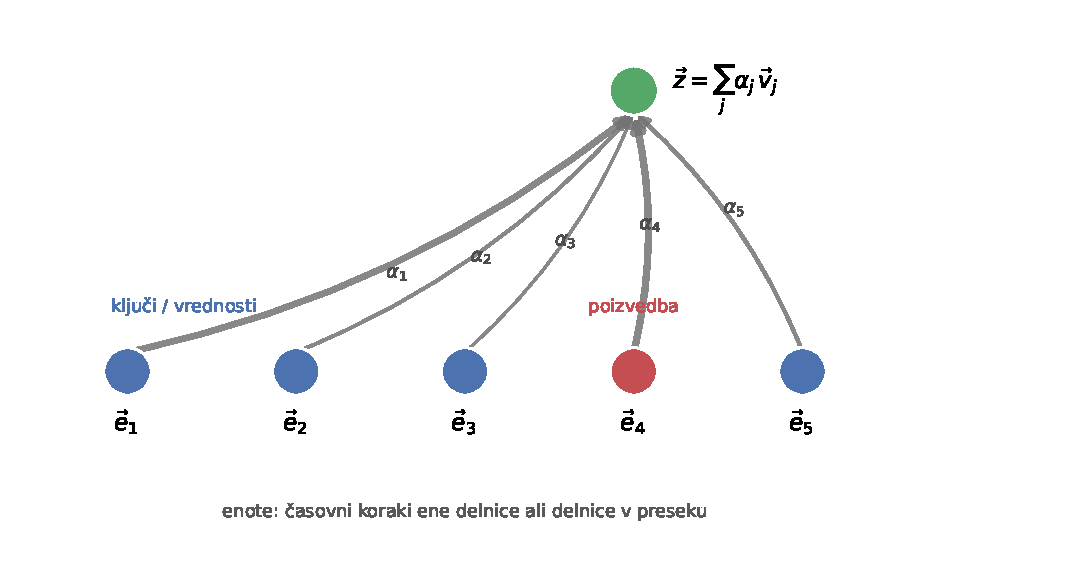
\includegraphics[width=0.78\linewidth]{transformer_pozornost}
  \caption{Mehanizem pozornosti: poizvedba (rdeča enota) svojo osveženo predstavitev~$\vec{z}$ sestavi kot uteženo vsoto vrednosti vseh enot, kjer so uteži~$\alpha_j$ (debelina puščic) sorazmerne podobnosti med poizvedbo in ključi.}
  \label{fig:attn}
\end{figure}

\newpage

%================================================================
\section{Napovedni transformerji za momenta donosov}
\label{sec:transformerji}

Namesto da bi zgradili lasten napovedni model, v tej nalogi uporabimo \textbf{tri že obstoječe (angl.\ \emph{off-the-shelf}) transformerske modele z javno dostopno kodo}, vsakega z drugačno oblikovno filozofijo, in jih z minimalnimi prilagoditvami vključimo v isti cevovod --- napoved momentov donosov, ki jo nato prevzame optimizator portfelja (Poglavje~\ref{ch:algoritmi}). Takšna zasnova ima tri prednosti: napovedi so \emph{ponovljive} (uporabimo objavljene izvedbe), izognemo se prekomernemu prilagajanju, ki bi ga prinesel bogat lasten model na naši zmerni univerzi sredstev, predvsem pa lahko \emph{pošteno ocenimo}, ali transformerji sploh prispevajo vrednost v primerjavi s klasičnimi ocenami.

Izbrani modeli pokrivajo tri komplementarne osi sodobnega napovedovanja:
\begin{itemize}
  \item \textbf{TACTiS-2}~\cite{ashok2024tactis} --- verjetnostni transformer, ki se nauči \emph{skupne} napovedne porazdelitve nad surovimi donosi vseh sredstev; edini izmed treh napove \emph{oba} momenta ($\vec{\mu}$ \emph{in} $\vec{\Sigma}$) iz iste porazdelitve.
  \item \textbf{MASTER}~\cite{li2024master} --- presečni tržno pogojeni transformer nad bogatim naborom tehničnih značilk; napove razvrstitveni signal $\vec{\mu}$.
  \item \textbf{TFT} (angl.\ \emph{Temporal Fusion Transformer})~\cite{lim2021tft} --- splošni večhorizontni napovedni transformer; napove $\vec{\mu}$.
\end{itemize}
Modela MASTER in TFT napovesta le $\vec{\mu}$; njuno matriko tveganja $\vec{\Sigma}$ ocenimo klasično (vzorčna kovarianca). Vse tri modele nato primerjamo čez več tržnih režimov (Poglavje~\ref{ch:eksperiment}).

\subsection{Osnovni pojmi}

\noindent\textbf{Presečna razvrstitev} (angl.\ \emph{cross-sectional ranking}): Pri izbiri portfelja ni ključna absolutna napoved donosa vsakega posameznega sredstva, temveč njihova relativna ureditev --- katera sredstva bodo v prihodnjem obdobju \emph{relativno} boljša (ali slabša) od drugih v naboru. Ker so donosi sredstev izrazito soodvisni prek skupnih makroekonomskih, tržnih in sektorskih dejavnikov, napredni modeli obravnavajo celoten presek sredstev \emph{hkrati} in med njimi neposredno modelirajo odvisnosti. Presečna razvrstitev tako preusmeri fokus iz napovedovanja točne številke na relativno hierarhijo, kar neposredno služi optimizatorju: za uspešno alokacijo kapitala ni pomembno, koliko je trg zrasel v absolutnem smislu, temveč katera sredstva nosijo največji relativni presežni donos (angl.\ \emph{alpha}).\\

\noindent\textbf{Informacijski koeficient} (IK; angl.\ \emph{information coefficient})~\cite{grinold2000}: Osrednja mera kakovosti napovedi, definirana kot presečna rang-korelacija med napovedanim signalom modela in dejansko uresničenim prihodnjim donosom čez celoten presek sredstev. IK neposredno meri prav to, kar za optimizacijo portfelja šteje: kako zanesljivo model loči zmagovalna sredstva od tistih, ki bodo prinesla izgubo.\\

\noindent\textbf{Verjetnostna napoved in kopula} (angl.\ \emph{probabilistic forecast, copula}): Namesto ene točkovne ocene lahko model napove celotno \emph{porazdelitev} prihodnjih donosov, iz katere lahko vzorčimo. Za več sredstev hkrati je poleg robnih porazdelitev posameznih donosov treba modelirati še njihovo \emph{soodvisnost}; ta struktura odvisnosti se matematično zajame s \emph{kopulo}. Iz vzorcev skupne porazdelitve lahko neposredno ocenimo oba momenta: $\vec{\mu}$ kot povprečje in $\vec{\Sigma}$ kot kovarianco vzorcev.\\

\noindent\textbf{Tržno pogojena vrata} (angl.\ \emph{market-guided gating}): Vektor dinamičnih uteži, ki ga model sproti izračuna iz \emph{tržnega konteksta} (stanje širokih indeksov, volatilnost, obseg trgovanja). Deluje kot inteligentni filter, ki glede na trenutni tržni režim poudari informativne dimenzije vhodnih predstavitev in zaduši prešumne.\\

\newpage

\subsection{TACTiS-2: transformer s pozornostno kopulo}
\label{sec:tactis}
Model \textbf{TACTiS-2} (angl.\ \emph{Transformer-Attentional Copulas for Time Series}) Ashoka in sod.~\cite{ashok2024tactis} je verjetnostni napovedni transformer, ki se nauči \emph{skupne} večrazsežne porazdelitve prihodnjih donosov vseh sredstev hkrati. Robne porazdelitve posameznih donosov modelira z normalizacijskim tokom, njihovo soodvisnost pa s \emph{pozornostno kopulo} --- kopulo, katere parametre generira mehanizem pozornosti. Model se uči v dveh fazah: najprej se naučijo robne porazdelitve, nato še kopula odvisnosti.

Momenta donosov iz modela pridobimo neposredno z vzorčenjem. Ob izbranem času $t$ modelu podamo okno zadnjih $\sim\!45$ dni surovih dnevnih donosov vseh sredstev; iz naučene skupne porazdelitve nato vzorčimo $S\!\approx\!400$ skupnih poti donosov za naslednjih $H$ dni. Vsako pot seštejemo v kumulativni $H$-dnevni donos, s čimer dobimo matriko vzorcev $\vec{C}\in\mathbb{R}^{N\times S}$. Momenta ocenimo kot vzorčno statistiko, kot podaja enačba~\eqref{eq:tactismoments}:
\begin{equation}
\label{eq:tactismoments}
  \vec{\mu} = \tfrac{1}{S}\textstyle\sum_{s} \vec{C}_{:,s}, \qquad
  \vec{\Sigma} = \operatorname{Cov}\!\big(\vec{C}\big).
\end{equation}
TACTiS-2 je torej \emph{edini} od naših modelov, ki poda oba momenta iz iste napovedane porazdelitve --- $\vec{\mu}$ z resnično magnitudo in $\vec{\Sigma}$, ki je z njo usklajena --- ne da bi karkoli prevzel iz zgodovinske ocene. Uporabimo ga prek javno dostopnega paketa \texttt{tactis}, kar zahteva le minimalne prilagoditve.

\subsection{MASTER: tržno pogojeni presečni transformer}
\label{sec:master}
Model \textbf{MASTER} (angl.\ \emph{Market-Guided Stock Transformer}) Lija in sod.~\cite{li2024master} je presečni transformer, zasnovan prav za napovedovanje razvrstitve donosov na celotnem preseku delnic. Uporabimo \emph{izvirno} izvedbo iz javnega repozitorija; njene vhodne značilke zgradimo sami iz cen in obsega trgovanja (OHLCV), tako da model teče na naši univerzi brez posebne podatkovne infrastrukture.

Vhod ob času $t$ za vsako sredstvo sestavlja okno zadnjih $L=8$ dni s $158$ tehničnimi značilkami (nabor \emph{Alpha158}: drseča povprečja, momentum, volatilnost, količinska razmerja ter korelacije cene z obsegom čez več časovnih oken) in $63$ tržnih značilk, ki napajajo tržno pogojena vrata (izpeljemo jih iz treh širokih indeksov). Model surove značilke najprej pretvori v predstavitev in jih modulira s tržnimi vrati, nato izvede \emph{časovno} pozornost (vzorci znotraj posamezne delnice), \emph{med-sredstveno} pozornost (relacije čez celoten presek delnic) in časovno agregacijo, na koncu pa iz predstavitve $\vec{z}_i$ z linearno preslikavo napove skalarni razvrstitveni signal $s_i$. Model se uči z minimizacijo srednje kvadratne napake na presečno standardiziranem prihodnjem donosu, kar v praksi ustreza razvrstitvenemu cilju. MASTER napove le $\vec{\mu}$ (razvrstitev); matriko tveganja $\vec{\Sigma}$ zanj ocenimo klasično.

\subsection{TFT: časovni fuzijski transformer}
\label{sec:tft}
Model \textbf{TFT} (angl.\ \emph{Temporal Fusion Transformer}) Lima in sod.~\cite{lim2021tft} je splošni večhorizontni napovedni transformer, ki ni zasnovan posebej za finance --- prav zato je pomemben preizkus, ali \emph{splošni} transformer sploh prispeva vrednost. Združuje mreže za \emph{izbor spremenljivk} (samodejno tehtajo pomen vhodnih značilk), \emph{vrata} za nadzor pretoka informacij, interpretabilno večglavo pozornost ter \emph{kvantilni} izhod (napove razpon, ne le točkovne vrednosti). Uporabimo ga prek javnega paketa \texttt{pytorch-forecasting}.

Vsakemu sredstvu podamo zaporedje dnevnih donosov z nekaj preprostimi kazalniki (momentum, volatilnost) in statično vložitev identitete delnice. Model napove \emph{naslednjih $H$ dnevnih donosov}; napovedani $H$-dnevni pričakovani donos posameznega sredstva dobimo kot vsoto teh napovedi (enaka definicija kot pri TACTiS-2). TFT napove le $\vec{\mu}$; $\vec{\Sigma}$ zanj ocenimo klasično.

\subsection{Vključitev v cevovod}
\label{sec:vkljucitev}
Modeli se razlikujejo v tem, kaj napovejo, zato jih v cevovod vključimo na dva načina. Za \textbf{TACTiS-2} $\vec{\mu}$ in $\vec{\Sigma}$ vzamemo neposredno iz napovedane porazdelitve (enačba~\eqref{eq:tactismoments}); nič ni prevzeto iz zgodovine. Za \textbf{MASTER} in \textbf{TFT} pa velja pomembna previdnost: njun signal je presečno \emph{normiran} in ne poda absolutne ravni donosa. Zato ga presečno standardiziramo in afino reskaliramo na povprečje ter razpršenost istočasne zgodovinske ocene~$\vec{\mu}$, kot povzema enačba~\eqref{eq:rescale}:
\begin{equation}
\label{eq:rescale}
  \vec{\mu}_{\text{model}} = \operatorname{zscore}(\vec{s})\cdot \sigma_{\vec{\mu}_{\text{hist}}} + \bar{\mu}_{\text{hist}}.
\end{equation}
S tem sta absolutna raven in razpon napovedi (in torej razmerje med donosom in tveganjem, ki ga vidi optimizator) enaka kot pri zgodovinskem scenariju; med scenariji se spreminja le presečni vrstni red sredstev, torej \emph{katera} sredstva so relativno privlačnejša. Prispevek teh dveh modelov je torej boljša razvrstitev, ne absolutna napoved donosa. Njuno matriko tveganja $\vec{\Sigma}$ ocenimo z vzorčno kovarianco. Za pošteno primerjavo TACTiS in TFT uporabljata \emph{enako} dolžino vhodnega okna (45 dni) kot drseči zgodovinski baseline; MASTER ohrani svoje izvirno okno 8 dni, saj njegove značilke Alpha158 v vsak korak že vgradijo daljšo zgodovino (drseče statistike do 60 dni).

V vseh primerih optimizator napovedi ne uporabi samostojno: pod kardinalno omejitvijo (največ $K$ sredstev) razvrstitev~$\vec{\mu}$ tehta proti oceni tveganja~$\vec{\Sigma}$ (Poglavje~\ref{ch:algoritmi}). Pri parametru tveganja~$P\!\to\!1$ bi sledil zgolj razvrstitvi (izbral najbolje uvrščena sredstva), sicer pa jo umeri z manjšanjem tveganja portfelja. Ključne lastnosti treh modelov povzema Tabela~\ref{tab:hp-model}.

\begin{table}[htbp]
  \centering
  \caption{Primerjava treh napovednih transformerjev.}
  \label{tab:hp-model}
  \small
  \begin{tabular}{lccc}
    \toprule
     & \textbf{TACTiS-2} & \textbf{MASTER} & \textbf{TFT}\\
    \midrule
    vir / paket        & \texttt{tactis} & izvirni repozitorij & \texttt{pytorch-forecasting}\\
    referenca          & \cite{ashok2024tactis} & \cite{li2024master} & \cite{lim2021tft}\\
    vhodne značilke    & surovi donosi & Alpha158 + tržne & donosi + kazalniki\\
    dolžina okna       & 45 dni & 8 dni & 45 dni\\
    izhod              & porazdelitev & razvrstitev & kvantili donosov\\
    napove $\vec{\mu}$ & da (vzorčno povpr.) & da (razvrstitev) & da (vsota donosov)\\
    napove $\vec{\Sigma}$ & \textbf{da} (vzorčna kov.) & ne & ne\\
    vključitev $\vec{\mu}$ & neposredno & reskaliran na zgod. & reskaliran na zgod.\\
    napovedni horizont & $H$ dni & $H$ dni & $H$ dni\\
    \bottomrule
  \end{tabular}
\end{table}

%================================================================
% Poglavje 4: Globalni optimizacijski algoritmi
%================================================================
\chapter{Globalni optimizacijski algoritmi}
\label{ch:algoritmi}

V razdelku~\ref{sec:ccmv} smo videli, da je kardinalno omejeni problem NP-težek: klasične kvadratne metode ga ne rešujejo, izčrpno preiskovanje vseh~$\binom{N}{K}$ naborov sredstev pa je za realistične~$N$ neizvedljivo. Kako torej najti dobro rešitev v sprejemljivem času? V tem poglavju najprej formaliziramo optimizacijski problem in razvrstimo pristope za njegovo reševanje, nato pa podrobno predstavimo tri metahevristike, ki jih uporabljamo. Vsako najprej opredelimo z definicijami ključnih pojmov, nato pa opišemo njeno izvajanje s psevdokodo.

\section{Globalna optimizacija in metahevristike}
\label{sec:globalna}

\paragraph{Optimizacijski problem.} \emph{Optimizacijski problem} je par~$(\mathcal{X}, c)$, kjer je~$\mathcal{X}$ \emph{dopustna množica} (množica vseh rešitev, ki zadostijo omejitvam problema), $c:\mathcal{X}\to\mathbb{R}$ pa \emph{kriterijska funkcija}. Iščemo
\begin{equation}
\label{eq:optprob}
  \vec{x}^\star = \arg\min_{\vec{x}\in\mathcal{X}} c(\vec{x}).
\end{equation}
Množici~$\mathcal{X}$ rečemo tudi \emph{prostor rešitev}. Za KOMV je~$\mathcal{X}$ množica vseh parov~$(\vec{w},\vec{z})$, ki zadostijo omejitvam~\eqref{eq:c-sum}--\eqref{eq:c-box}, $c$ pa negativni mean-variance kriterij~\eqref{eq:objective}; ker je izbir sredstev~$\binom{N}{K}$, je prostor rešitev kombinatorično velik.

\paragraph{Globalni in lokalni optimum.} Rešitev~$\vec{x}^\star\in\mathcal{X}$ je \emph{globalni optimum}, če velja~$c(\vec{x}^\star)\le c(\vec{x})$ za vse~$\vec{x}\in\mathcal{X}$. \emph{Sosednost}~$\mathcal{N}(\vec{x})\subseteq\mathcal{X}$ je množica rešitev, ki jih iz~$\vec{x}$ dosežemo z eno elementarno potezo (npr.\ zamenjavo enega izbranega sredstva). Rešitev~$\vec{x}$ je \emph{lokalni optimum} glede na~$\mathcal{N}$, če velja~$c(\vec{x})\le c(\vec{x}')$ za vse~$\vec{x}'\in\mathcal{N}(\vec{x})$. Glavna težava preproste ``pohlepne'' optimizacije je, da obtiči v lokalnem optimumu, ki ni globalni; dobra metoda mora zato prostor rešitev \emph{raziskovati}, ne le \emph{izkoriščati} trenutno najboljše okolice.

\begin{primer}
\label{pr:optimum}
Slika~\ref{fig:pr-opt} prikazuje kriterijsko funkcijo~$c$ z več minimumi. Pohlepen postopek, ki vedno sprejme le izboljšave, se iz začetne rešitve spusti v najbližji minimum in tam obtiči --- lokalni optimum (oranžno), ki pa ni globalni (rdeče). Da bi našli globalni optimum, mora postopek občasno sprejeti tudi slabšo rešitev in tako preiti ``hrib'' med minimumoma; ta zmožnost je bistvo metahevristik, ki jih obravnavamo v nadaljevanju.
\end{primer}

\begin{figure}[htbp]
  \centering
  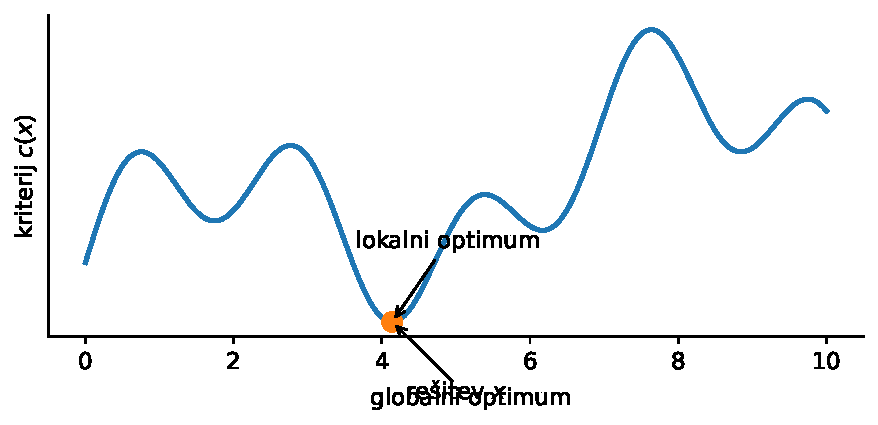
\includegraphics[width=0.72\linewidth]{primer_optimum}
  \caption{Lokalni in globalni optimum kriterijske funkcije z več minimumi. Pohlepno lokalno iskanje obtiči v lokalnem optimumu; metahevristike znajo pobegniti proti globalnemu.}
  \label{fig:pr-opt}
\end{figure}

\paragraph{Razvrstitev pristopov.} Metode globalne optimizacije v grobem delimo na \emph{deterministične} (pri istem vhodu vedno vrnejo isti rezultat; zanesljive, a za velike prostore rešitev pogosto neizvedljive) in \emph{stohastične} (prostor preiskujejo naključno; za isti vhod ne vrnejo nujno istega rezultata, a so za velike prostore uporabnejše). Najpreprostejši stohastični pristop je \emph{popolnoma naključno iskanje}, ki zgenerira~$N$ naključnih rešitev in izbere najboljšo; njegova slabost je, da ne izkorišča že najdenih dobrih rešitev.

\paragraph{Metahevristike.} \emph{Metahevristika} je splošna stohastična strategija iskanja, ki uravnava razmerje med raziskovanjem (angl.\ \emph{exploration}) in izkoriščanjem (angl.\ \emph{exploitation}) ter jo je mogoče uporabiti za širok razred problemov. Glede na to, koliko rešitev hkrati vzdržujejo, jih delimo na:
\begin{itemize}
  \item \emph{postopke lokalnega iskanja}, ki vzdržujejo eno samo trenutno rešitev in se premikajo po njeni sosednosti (npr.\ simulirano ohlajanje);
  \item \emph{populacijske postopke}, ki vzdržujejo množico (populacijo) rešitev in jih razvijajo skupaj (npr.\ rojenje delcev in genetski algoritem).
\end{itemize}
Vse metahevristike sledijo skupni shemi: (i)~\emph{inicializacija} začetne rešitve ali populacije, (ii)~\emph{iteracija}, v kateri z naključnimi potezami generiramo nove kandidatne rešitve, jih ovrednotimo s kriterijsko funkcijo in izberemo, katere obdržimo, ter (iii)~\emph{ustavitev} ob izpolnjenem končnem pogoju. Ključno je, da uravnavajo razmerje med raziskovanjem (da se izognejo lokalnim optimumom) in izkoriščanjem (da izboljšujejo dobre rešitve). V nadaljevanju predstavimo tri uveljavljene metahevristike, vsako v izvedbi, zvesti izvirnemu članku.

\section{Skupni okvir}
\label{sec:okvir}

Vsi trije algoritmi minimizirajo isto \emph{kriterijsko funkcijo} --- negativni mean-variance kriterij
\begin{equation}
\label{eq:objective}
  c(\vec{w}) = -\big(P\,\vec{\mu}^{\!\top}\vec{w} - (1-P)\,\vec{w}^{\!\top}\vec{\Sigma}\vec{w}\big),
\end{equation}
pod kardinalno omejitvijo~$K$ in mejami uteži~$[\varepsilon_i,\delta_i]$. Rešitev predstavimo z \emph{indikatorskim} vektorjem~$\vec{z}\in\{0,1\}^N$ (katera sredstva so izbrana) in vektorjem uteži~$\vec{w}$. Ker morajo rešitve zadostiti omejitvam, vsak algoritem uporablja \emph{popravilo} (angl.\ \emph{repair}): postopek, ki poljubno rešitev projicira na dopustno množico tako, da število izbranih sredstev uravna na~$K$ in uteži normira, da vsota znaša~1 ob upoštevanju mej. Pomembno je, da vse tri izvedbe uporabljajo \emph{izključno naključne} poteze pri iskanju (brez uporabe~$\vec{\mu}$ ali~$\vec{\Sigma}$ v samem koraku iskanja), tako da napovedni signal vstopi le prek kriterijske funkcije~\eqref{eq:objective}. S tem ostane primerjava med zgodovinskim in transformerskim~$\vec{\mu}$ čista.

\begin{primer}
\label{pr:kard}
Slika~\ref{fig:pr-kard} ponazarja popravilo pri~$K=4$. Levo je rešitev z osmimi neničelnimi utežmi (krši kardinalno omejitev). Popravilo obdrži~$K=4$ sredstva z največjimi utežmi, ostala nastavi na nič in preostale uteži normira, da se seštejejo v~1 (desno). Vsaka ovrednotena rešitev ima torej natanko~$K$ neničelnih uteži --- prav zato ima portfelj v \emph{vsakem} walk-forward oknu natanko~$K$ sredstev, čeprav se izbrana množica med okni spreminja.
\end{primer}

\begin{figure}[htbp]
  \centering
  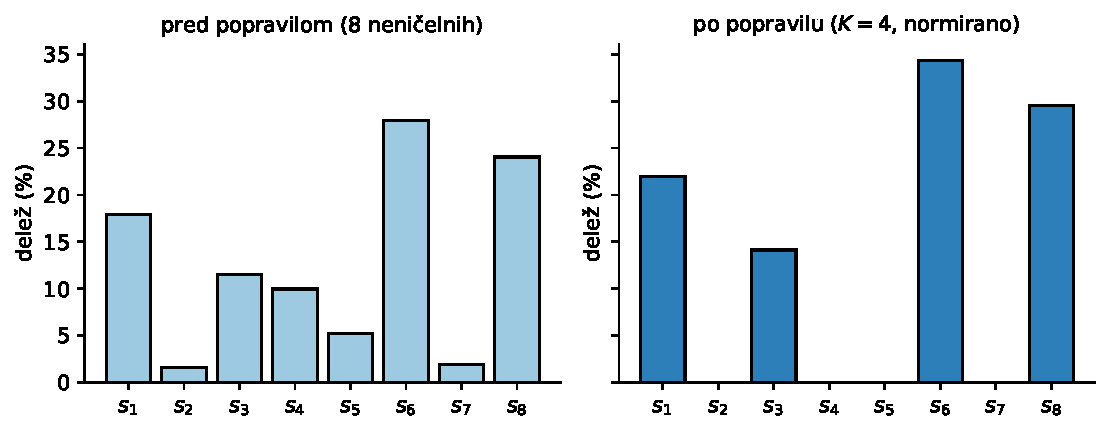
\includegraphics[width=0.8\linewidth]{primer_kardinalnost}
  \caption{Popravilo na kardinalno omejitev ($K{=}4$): rešitev z osmimi neničelnimi utežmi (levo) se projicira na štiri največje, ki se normirajo v vsoto~1 (desno).}
  \label{fig:pr-kard}
\end{figure}

\section{Rojenje delcev}
\label{sec:pso}

Rojenje delcev (RD; angl.\ \emph{particle swarm optimization}; Kennedy in Eberhart~\cite{kennedy1995}) posnema gibanje jate: populacija ``delcev'' se giblje po prostoru rešitev, vsak pod vplivom svoje in skupinske izkušnje. Sledimo izvedbi Cure~\cite{cura2009}, prilagojeni kardinalni omejitvi.

\subsection{Definicije}
\emph{Delec} je kandidatna rešitev, ki jo opišemo z indikatorskim vektorjem~$\vec{z}$ in vektorjem uteži~$\vec{w}$. \emph{Hitrost} delca sta vektorja~$\vec{v}_z$ in~$\vec{v}_w$, ki določata spremembo indikatorjev oziroma uteži v naslednji iteraciji. \emph{Osebni najboljši} položaj je najboljša rešitev, ki jo je delec doslej obiskal, \emph{globalni najboljši} pa najboljša rešitev celotne populacije. \emph{Izbirna mera} (Cura) je za vsako sredstvo vnaprej izračunana ocena privlačnosti (razmerje med prispevkom k donosu in prispevkom k tveganju), ki jo uporablja postopek popravila. \emph{Popravilo (arrange)} indikatorje uravna na~$K$: sredstva dodaja oziroma odstranjuje, pri čemer se z verjetnostjo~$\tfrac12$ odloči naključno, sicer pa po izbirni meri (doda najprivlačnejše, odstrani najmanj privlačno).

\subsection{Izvajanje RD}
Postopek povzema Algoritem~\ref{alg:pso}. Delci se inicializirajo naključno in popravijo na~$K$ sredstev. V vsaki iteraciji vsak delec posodobi hitrost kot uteženo kombinacijo privlačnosti k osebnemu in globalnemu najboljšemu (s koeficientoma~$\omega_1,\omega_2$, vzorčenima iz~$U[0,2]$), nato posodobi indikatorje (prek sigmoidne funkcije praga) in uteži, se popravi na dopustno rešitev ter ovrednoti. Če je nova rešitev boljša od osebnega oziroma globalnega najboljšega, se ta posodobi.

\begin{algorithm}[htbp]
\caption{Rojenje delcev (RD) za KOMV}
\label{alg:pso}
\begin{algorithmic}[1]
\footnotesize
\REQUIRE $\vec{\mu}$, $\vec{\Sigma}$, kardinalnost $K$, velikost populacije $P$, št.\ generacij $G$
\ENSURE portfelj $\vec{w}^\star$
\STATE predizračunaj izbirno mero $c_i$ za vsa sredstva
\FOR{vsak delec $p=1,\dots,P$}
  \STATE naključno izberi $K$ sredstev, nastavi uteži; popravi na dopustno rešitev
  \STATE ovrednoti $c(\vec{w}_p)$; osebni najboljši $\gets$ trenutni
\ENDFOR
\STATE globalni najboljši $\gets$ najboljši delec
\FOR{iteracijo $=1,\dots,\lfloor G\cdot P / P\rfloor$}
  \FOR{vsak delec $p$}
    \STATE vzorči $\omega_1,\omega_2 \sim U[0,2]$
    \STATE posodobi hitrost in indikatorje $\vec{z}_p$ (sigmoidni prag), nato uteži $\vec{w}_p$
    \STATE popravi $\vec{z}_p,\vec{w}_p$ na dopustno rešitev (\emph{arrange})
    \STATE ovrednoti $c(\vec{w}_p)$
    \IF{boljši od osebnega najboljšega} \STATE posodobi osebni najboljši \ENDIF
    \IF{boljši od globalnega najboljšega} \STATE posodobi globalni najboljši \ENDIF
  \ENDFOR
\ENDFOR
\RETURN uteži globalnega najboljšega
\end{algorithmic}
\end{algorithm}

\begin{primer}
\label{pr:pso}
Slika~\ref{fig:pr-pso} ponazarja premik enega delca v (poenostavljenem dvorazsežnem) prostoru rešitev, katerega izolinije prikazujejo kriterijsko funkcijo. Delec (moder) se premakne pod vplivom dveh privlačnosti: k svojemu osebnemu najboljšemu položaju (oranžno) in h globalnemu najboljšemu položaju roja (rdeče). Novi položaj (zeleno) je vsota trenutne hitrosti in obeh privlačnosti, uteženih z naključnima koeficientoma~$\omega_1,\omega_2\sim U[0,2]$. Roj tako postopoma konvergira proti obetavnim območjem, hkrati pa naključnost ohranja raziskovanje.
\end{primer}

\begin{figure}[htbp]
  \centering
  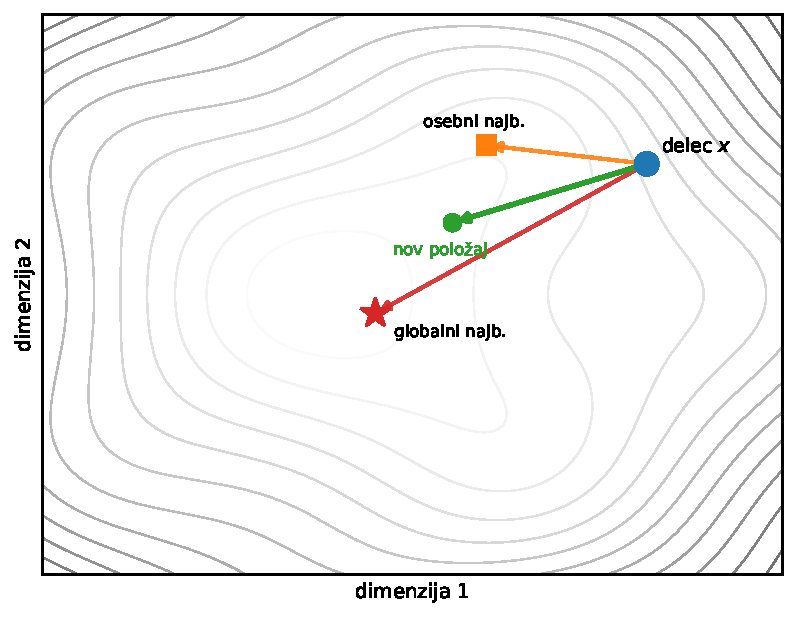
\includegraphics[width=0.62\linewidth]{primer_pso}
  \caption{Premik delca pri rojenju delcev: delec se giblje pod vplivom privlačnosti k osebnemu (oranžno) in globalnemu (rdeče) najboljšemu položaju; rezultat je nov položaj (zeleno).}
  \label{fig:pr-pso}
\end{figure}

\section{Simulirano ohlajanje}
\label{sec:sa}

Simulirano ohlajanje (SO; angl.\ \emph{simulated annealing}; Kirkpatrick in sod.~\cite{kirkpatrick1983}) izvira iz metalurgije: na začetku sprejema tudi slabše rešitve, z nižanjem ``temperature'' pa postaja vse bolj selektivno. Sledimo izvedbi Crame in Schynsa~\cite{cramaschyns2003}.

\subsection{Definicije}
\emph{Temperatura}~$T$ določa verjetnost, s katero algoritem sprejme slabšo rešitev: pri višji temperaturi z večjo verjetnostjo. \emph{Temperaturni urnik} tvorita začetna temperatura~$T_0$ in način nižanja; uporabimo geometrijsko ohlajanje~$T' \gets \alpha\,T$ s faktorjem~$\alpha\in(0,1)$. \emph{Sosednostna funkcija} iz trenutne rešitve tvori natanko eno sosednjo (v našem primeru z naključno zamenjavo enega izbranega sredstva za neizbrano ali s premikom uteži). \emph{Verjetnostna funkcija} določi, ali novo rešitev sprejmemo: če je boljša, jo vedno sprejmemo, sicer pa z verjetnostjo~$\exp(-\Delta/T)$, kjer je~$\Delta>0$ poslabšanje kriterija. \emph{Končni pogoj} ustavi postopek, ko dosežemo najnižjo temperaturo ali največje število iteracij.

\subsection{Izvajanje SO}
Postopek povzema Algoritem~\ref{alg:sa}. Iz naključne začetne rešitve v vsaki iteraciji s sosednostno funkcijo tvorimo novo rešitev; boljšo sprejmemo vedno, slabšo pa z verjetnostjo, odvisno od poslabšanja in trenutne temperature. Po vsakem koraku temperaturo znižamo.

\begin{algorithm}[htbp]
\caption{Simulirano ohlajanje (SO) za KOMV}
\label{alg:sa}
\begin{algorithmic}[1]
\footnotesize
\REQUIRE $\vec{\mu}$, $\vec{\Sigma}$, $K$, začetna temp.\ $T_0$, min.\ temp.\ $T_{\min}$, faktor $\alpha$
\ENSURE portfelj $\vec{w}^\star$
\STATE $\vec{w} \gets$ naključna dopustna rešitev; $\vec{w}^\star \gets \vec{w}$; $T \gets T_0$
\WHILE{$T > T_{\min}$ in ni doseženo max.\ iteracij}
  \STATE $\vec{w}' \gets$ sosednostna funkcija($\vec{w}$) \COMMENT{naključna poteza + popravilo}
  \STATE $\Delta \gets c(\vec{w}') - c(\vec{w})$
  \IF{$\Delta < 0$}
    \STATE $\vec{w} \gets \vec{w}'$; \textbf{če} $c(\vec{w}') < c(\vec{w}^\star)$ \textbf{potem} $\vec{w}^\star \gets \vec{w}'$
  \ELSE
    \STATE $r \gets \mathrm{rand}(0,1)$; \textbf{če} $\exp(-\Delta/T) > r$ \textbf{potem} $\vec{w} \gets \vec{w}'$
  \ENDIF
  \STATE $T \gets \alpha\,T$ \COMMENT{geometrijsko ohlajanje}
\ENDWHILE
\RETURN $\vec{w}^\star$
\end{algorithmic}
\end{algorithm}

\begin{primer}
\label{pr:sa}
Slika~\ref{fig:pr-sa} prikazuje verjetnost sprejema slabše rešitve~$e^{-\Delta/T}$ v odvisnosti od poslabšanja~$\Delta$ pri treh temperaturah. Pri visoki temperaturi ($T=1$) algoritem z veliko verjetnostjo sprejme tudi občutno slabše rešitve in tako široko raziskuje prostor; z nižanjem temperature ($T=0{,}2$, nato~$T=0{,}05$) postaja vse bolj selektiven in sprejema le še majhna poslabšanja. Temperaturni urnik torej gladko preide iz raziskovanja v izkoriščanje.
\end{primer}

\begin{figure}[htbp]
  \centering
  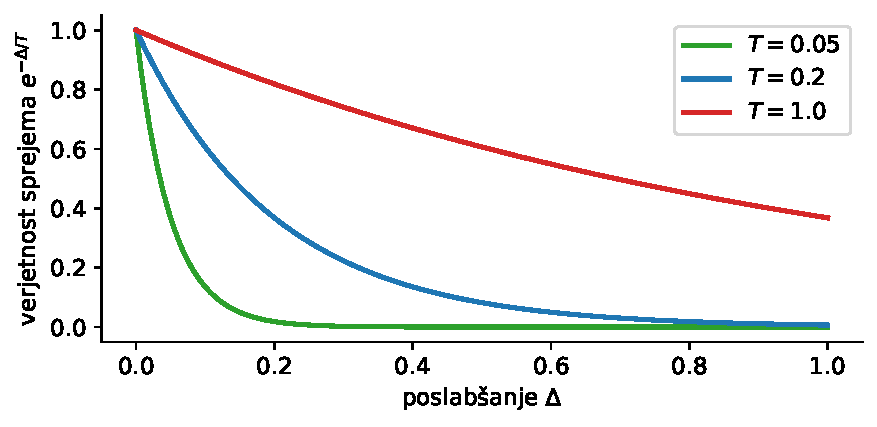
\includegraphics[width=0.72\linewidth]{primer_sa_sprejem}
  \caption{Verjetnost sprejema slabše rešitve $e^{-\Delta/T}$ pri simuliranem ohlajanju za tri temperature. Nižja temperatura pomeni bolj selektivno sprejemanje.}
  \label{fig:pr-sa}
\end{figure}

\section{Genetski algoritem}
\label{sec:ga}

Genetski algoritem (GA; angl.\ \emph{genetic algorithm}; Goldberg~\cite{goldberg1989}) posnema mikroevolucijo: populacija rešitev se z izborom, križanjem in mutacijo v zaporednih generacijah razvija proti optimumu. Sledimo izvedbi Changa in sod.~\cite{chang2000}.

\subsection{Definicije}
\emph{Kromosom} (posameznik) je kandidatna rešitev; kodiramo ga z množico izbranih sredstev~$Q$ in vektorjem deležev~$\vec{s}$, iz katerih z \emph{dekodiranjem} (vodno-polnilna projekcija) dobimo dopustne uteži~$\vec{w}$. \emph{Kriterijska funkcija} je vrednost~\eqref{eq:objective} dekodiranega kromosoma. \emph{Izbor po kolesu sreče} izbere starša z verjetnostjo, sorazmerno njegovi kakovosti (boljši kromosomi imajo večjo verjetnost). \emph{Enakomerno križanje} otroka sestavi tako, da vsako sredstvo neodvisno podeduje od enega od staršev. \emph{Mutacija} z majhno verjetnostjo spremeni deleže ali zamenja izbrano sredstvo. Uporabimo \emph{stabilnostno} (angl.\ \emph{steady-state}) različico, kjer vsaka iteracija ustvari enega otroka, ki zamenja najslabšega člana populacije, če je boljši od njega.

\subsection{Izvajanje GA}
Postopek povzema Algoritem~\ref{alg:ga}. Populacijo naključno inicializiramo. V vsaki iteraciji z izborom po kolesu sreče izberemo dva starša, ju z enakomernim križanjem in mutacijo združimo v otroka, ga dekodiramo in ovrednotimo ter z njim zamenjamo najslabšega člana, če je boljši.

\begin{algorithm}[htbp]
\caption{Genetski algoritem (GA) za KOMV}
\label{alg:ga}
\begin{algorithmic}[1]
\footnotesize
\REQUIRE $\vec{\mu}$, $\vec{\Sigma}$, $K$, velikost populacije $\mathit{NP}$, št.\ generacij $G$
\ENSURE portfelj $\vec{w}^\star$
\STATE inicializiraj populacijo naključnih kromosomov; dekodiraj in ovrednoti
\STATE globalni najboljši $\gets$ najboljši kromosom
\FOR{iteracijo $=1,\dots,\mathit{NP}\cdot G$}
  \STATE $s_1,s_2 \gets$ izbor po kolesu sreče (dva starša)
  \STATE otrok $\gets$ enakomerno križanje($s_1,s_2$); popravi na $K$ sredstev
  \STATE mutiraj otroka (deleži in/ali zamenjava sredstva)
  \STATE dekodiraj in ovrednoti otroka
  \STATE zamenjaj najslabšega člana populacije z otrokom, če je boljši
  \STATE posodobi globalni najboljši, če je otrok boljši
\ENDFOR
\RETURN uteži globalnega najboljšega
\end{algorithmic}
\end{algorithm}

\begin{primer}
\label{pr:ga}
Slika~\ref{fig:pr-ga} ponazarja križanje in mutacijo pri~$N=8$ sredstvih. Modre celice pomenijo izbrana sredstva. Iz dveh staršev z \emph{enakomernim križanjem} sestavimo otroka, tako da vsako sredstvo neodvisno podeduje od enega od staršev. Otroka nato \emph{mutiramo}: eno izbrano sredstvo odstranimo in namesto njega izberemo drugega (rdeče označeni celici). Mutacija vnese raznolikost, ki postopku pomaga uiti lokalnim optimumom.
\end{primer}

\begin{figure}[htbp]
  \centering
  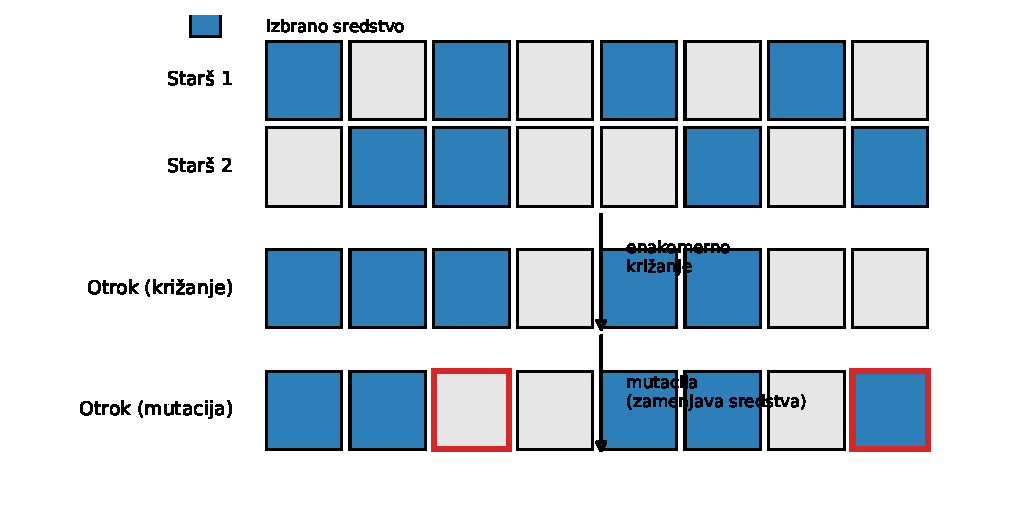
\includegraphics[width=0.82\linewidth]{primer_ga}
  \caption{Enakomerno križanje in mutacija pri genetskem algoritmu. Otrok podeduje izbor sredstev od obeh staršev; mutacija nato zamenja eno izbrano sredstvo (rdeče).}
  \label{fig:pr-ga}
\end{figure}

\section{Implementacija in nastavitve optimizatorjev}
\label{sec:impl-opt}

Metahevristike so implementirane v jeziku C++ kot en sam prevajalni sklop, ki vključuje vse tri algoritme in skupno redko-zasedeno ciljno funkcijo ter popravilo uteži. Napovedni model (Poglavje~\ref{ch:model}) v jeziku Python izračuna~$\vec{\mu}$ in~$\vec{\Sigma}$, ju zapiše v datoteko JSON in pokliče prevedeni binarni program; ta reši izbrani algoritem in rešitev vrne na standardni izhod, od koder Python razčleni uteži. Takšna ločitev prek datotek je preprosta in neodvisna od jezikovnih vezav.

\paragraph{Redko-zasedena ciljna funkcija.} Ciljno funkcijo~\eqref{eq:objective} optimizator ovrednoti ob vsakem koraku iskanja, zato je njena hitrost ključna. Ker pri kardinalnosti~$K$ prispeva le~$K$ neničelnih uteži, kvadratno obliko~$\vec{w}^{\!\top}\vec{\Sigma}\vec{w}$ računamo zgolj čez neničelne indekse, v času~$O(N+K^2)$ namesto~$O(N^2)$. Podobno predizračunamo Cura-jevo izbirno mero za RD enkrat na klic optimizatorja, saj je odvisna le od~$\vec{\mu}$,~$\vec{\Sigma}$ in~$\lambda$, ki so v oknu fiksni. Ti pohitritvi sta \emph{matematično nevtralni}: vrednosti ciljne funkcije ostanejo enake (do zaokroževanja s plavajočo vejico), zato ne spremenita rezultatov, kar smo potrdili na knjižnici OR-Library (napaka fronte ostane enaka do štirih decimalk).

\paragraph{Hiperparametri.} Za ponovljivost Tabela~\ref{tab:hp-solver} navaja vse hiperparametre optimizatorjev; problemske omejitve (kardinalnost~$K$, meje uteži, parameter tveganja~$P$) so podane pri posameznem poskusu v Poglavju~\ref{ch:eksperiment}.

\begin{table}[htbp]
  \centering
  \caption{Hiperparametri metahevristik (skupni ter po algoritmih).}
  \label{tab:hp-solver}
  \begin{tabular}{lll}
    \toprule
    Algoritem & Parameter & Vrednost\\
    \midrule
    skupno & velikost populacije & 200\\
           & št.\ generacij      & 1500\\
           & naključno seme                & 42\\
    \midrule
    RD    & $\alpha$ (Cura~\cite{cura2009}) & 0{,}06\\
           & $\omega_1,\omega_2$ & $\sim U[0,2]$\\
    \midrule
    SO     & faktor ohlajanja $\alpha$ & 0{,}95\\
           & začetna verj.\ sprejema   & 0{,}8\\
           & faktor dolžine stopnje     & 2\\
           & št.\ ustavitvenih stopenj  & 5\\
    \midrule
    GA     & verjetnost mutacije & 0{,}01\\
           & $\sigma$ mutacije    & 0{,}05\\
           & izbor / križanje     & kolo sreče / enakomerno\\
    \bottomrule
  \end{tabular}
\end{table}

%================================================================
% Poglavje 5: Eksperimentalno vrednotenje
%================================================================
\chapter{Eksperimentalno vrednotenje}
\label{ch:eksperiment}

V tem poglavju povežemo napovedni model (Poglavje~\ref{ch:model}) in optimizacijske algoritme (Poglavje~\ref{ch:algoritmi}) v celoten cevovod ter ga ovrednotimo. Najprej opišemo cevovod, scenarije in postopek vrednotenja skupaj s statistično metodologijo, nato pa predstavimo rezultate: neodvisno preverbo kakovosti optimizatorjev na knjižnici OR-Library, kakovost napovedi, robustnost čez tržne režime, združeni preizkus značilnosti in neposredni primerjavi na tujih protokolih. Sledi podroben pregled po posameznih režimih, poglavje pa sklenemo s pošteno predstavitvijo poti do končne zasnove in opombo o ponovljivosti.

\section{Cevovod, scenariji in referenčne strategije}
\label{sec:pregled}

Sistem je razdeljen na tri sklope. \emph{Ocenjevalniki} (paket \texttt{estimators}) vsebujejo napovedni model~$\vec{\mu}$/$\vec{\Sigma}$ (presečni transformer iz Poglavja~\ref{ch:model}) in spletni ansambel. \emph{Optimizatorji} (mapa \texttt{portfolio\_optimizers}) so implementirani v C++ (razdelek~\ref{sec:impl-opt}). \emph{Orkestracija} (paket \texttt{benchmark}) izvaja postopno zanko, poganja optimizatorje, računa referenčne strategije in izvozi rezultate ter statistiko. Klasične strategije brez~$\vec{\mu}$ (GMV, paritet tveganja, HPT) in tangentni Markowitz so implementirane ločeno v jeziku Python, saj gre za zaprte oziroma konveksne rešitve, ki jih ni treba prepuščati metahevristikam.

Cevovod v vsakem obdobju iz zgodovine cen izračuna oceni~$\vec{\mu}$ in~$\vec{\Sigma}$ ter ju preda metahevristikam, ki rešijo problem~\eqref{eq:ccmv}. Osrednja primerjava poteka med tremi \emph{scenariji}, od katerih vsak sestavlja svoj celoten cevovod z domorodno oceno kovariance:
\begin{itemize}
  \item \textbf{Zgodovinski:}~$\vec{\mu}$ je drseče vzorčno povprečje donosov, $\vec{\Sigma}$ pa vzorčna kovarianca --- povsem klasična referenca.
  \item \textbf{Transformer:} oba momenta izhajata iz presečnega transformerja (napovedna~$\vec{\mu}$-veja in faktorska~$\vec{\Sigma}$-veja iz iste deljene predstavitve).
  \item \textbf{Ansambel:} postopek Hedge (Algoritem~\ref{alg:hedge}) spletno kombinira transformerski in zgodovinski~$\vec{\mu}$ v~$\vec{\mu}_{\text{ans}}$, medtem ko transformerjeva~$\vec{\Sigma}$ ansambel obide in gre neposredno v optimizator.
\end{itemize}
Ker vsak scenarij uporablja svojo domorodno~$\vec{\Sigma}$, primerjava meri \emph{celotne pristope}, ne le vira~$\vec{\mu}$ v izolaciji. Vsi trije scenariji svoje momente predajo istim metahevristikam. Slika~\ref{fig:cevovod} povzame celoten cevovod.

\begin{figure}[htbp]
  \centering
  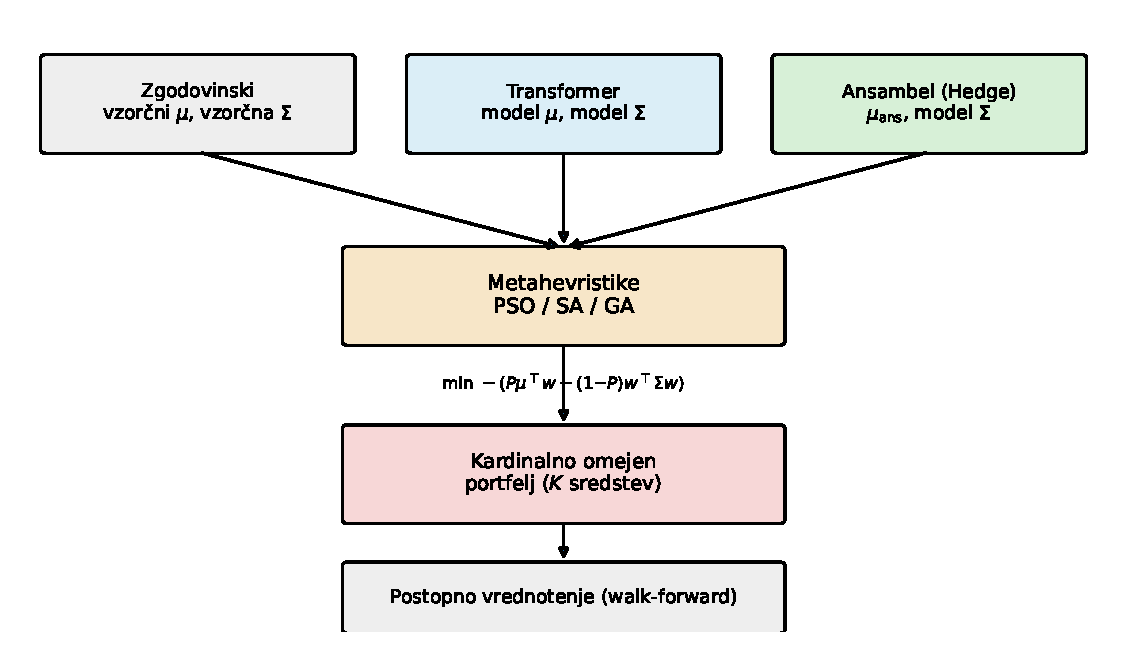
\includegraphics[width=0.86\linewidth]{cevovod_shema}
  \caption{Shema cevovoda: vsak od treh scenarijev proizvede oceni~$\vec{\mu}$ in~$\vec{\Sigma}$, ki ju iste metahevristike (RD/SO/GA) uporabijo za reševanje kardinalno omejenega mean-variance problema; dobljeni portfelj ovrednotimo postopno (walk-forward).}
  \label{fig:cevovod}
\end{figure}

\paragraph{Dinamični parameter tveganja.}\label{sec:dynp}
Parameter~$P$ v~\eqref{eq:mvobj} prilagajamo tržnemu režimu po logiki Anga in Bekaerta~\cite{ang2004}, ki pokažeta, da investitor, ki ignorira volatilnostne režime, v visoko-volatilnem (medvedjem) obdobju drži preveč tveganih sredstev. Naj bo~$\sigma_{21}$ 21-dnevna realizirana volatilnost trga v danem oknu ter~$\sigma_{\text{lo}}$ in~$\sigma_{\text{hi}}$ spodnji in zgornji prag. Parameter~$P$ zvezno interpoliramo med~$P_0-\Delta$ (visoka volatilnost) in~$P_0+\Delta$ (nizka volatilnost):
\begin{equation}
\label{eq:dynp}
  P(\sigma_{21}) = P_0 - \Delta + 2\Delta\cdot\mathrm{clip}\!\left(\frac{\sigma_{\text{hi}}-\sigma_{21}}{\sigma_{\text{hi}}-\sigma_{\text{lo}}},\,0,\,1\right).
\end{equation}
V nizko-volatilnem (bikovskem) režimu ima mean-variance fronta višji Sharpe, zato v~\eqref{eq:dynp} bolj zaupamo napovedi~$\vec{\mu}$ (višji~$P$); v visoko-volatilnem režimu so napovedi manj zanesljive (nižji~$P$).

\paragraph{Primerjalne strategije.}\label{sec:baselines}
Poleg treh scenarijev vpeljemo vrsto primerjalnih strategij, ki izolirajo posamezne zasnovne odločitve:
\begin{itemize}
  \item \textbf{Naivne:} enakomerni portfelj~$1/N$ ter~$1/N$ na~$K$ najboljših po napovedi. DeMiguel in sod.~\cite{demiguel2009} opozarjajo, da je naivni~$1/N$ v končnih vzorcih presenetljivo težko premagati.
  \item \textbf{Zgolj na~$\vec{\Sigma}$ (brez~$\vec{\mu}$):} globalni minimalno-variančni portfelj (GMV), paritet tveganja in hierarhični paritet tveganja (HPT)~\cite{lopezdeprado2016}. Če jih napovedni scenarij premaga, to potrjuje vrednost napovedi~$\vec{\mu}$.
  \item \textbf{Brez kardinalnosti:} Markowitzev tangentni portfelj z istim~$\vec{\mu}$ in~$\vec{\Sigma}$, a brez kardinalne omejitve --- izolira ceno omejitve in metahevristike.
  \item \textbf{Močne napovedne reference} (z Ledoit-Wolf skrčeno~\cite{ledoit2004} kovarianco): gradientni gozd~\cite{ke2017lightgbm} kot preprost strojni~$\vec{\mu}$, Black-Litterman (BL)~\cite{black1992} kot klasičen bayesovski~$\vec{\mu}$ in sekvenčni LSTM~\cite{hochreiter1997lstm} kot alternativna nevronska arhitektura. Te reference so \emph{strožje} od vzorčne, saj sta Ledoit-Wolf skrčenje in strojni~$\vec{\mu}$ močnejša od naivnih.
  \item \textbf{Pasivna:} tržni indeks (nakup-in-drži) z zanemarljivim obratom.
\end{itemize}

\paragraph{Podatki in konfiguracija.}\label{sec:config}
Zgodovinske prilagojene zaključne cene in obseg trgovanja pridobimo prek storitve \texttt{yfinance}. Iz njih izpeljemo vhodne značilke in tarče, kot je opisano v Poglavju~\ref{ch:model} (razdelek o gradnji značilk). Konfiguracija je razdeljena po odgovornosti na dve datoteki, ki se ob zagonu združita: \emph{eksperimentalna} konfiguracija (nabor sredstev, testno obdobje, hiperparametri napovednega modela, definicija problema~$K$/$\varepsilon$/$\delta$/$P$, nastavitve ansambla) in \emph{solverska} konfiguracija (velikost populacije, število generacij, naključno seme in parametri posameznih algoritmov iz Tabele~\ref{tab:hp-solver}). Takšna delitev omogoča, da solverske parametre nastavimo enkrat in jih delimo med vsemi poskusi, medtem ko se eksperimentalna definicija spreminja po režimu. Vsi hiperparametri napovednega modela so zbrani v Tabeli~\ref{tab:hp-model}, hiperparametri optimizatorjev pa v Tabeli~\ref{tab:hp-solver}.

\section{Postopno vrednotenje in statistična značilnost}
\label{sec:walkforward}

Celoten cevovod ovrednotimo s \emph{postopnim} (walk-forward) testiranjem, ki posnema realno rabo: v vsakem trenutku uporabimo le pretekle podatke.

\paragraph{Postopek.} Napovedni model naučimo na obdobju pred testom. Testno obdobje razdelimo na~$W$ zaporednih, neprekrivajočih (mesečnih) oken. Za vsako okno na \emph{rastoči} zgodovini izračunamo~$\vec{\mu}$ in~$\vec{\Sigma}$, rešimo optimizacijo in dobljeni portfelj ovrednotimo na donosih \emph{naslednjega} okna. Zgodovinske ocene se kotalijo prek istega nedavnega okna, kot ga transformer vidi pri inferenci, kar zagotavlja pošteno primerjavo.

\paragraph{Kavzalnost in razmejitev.} Ključno je, da model \emph{nikoli ne vidi testnih podatkov}. To zagotovimo z: (i)~učnim obdobjem, ki se konča strogo pred prvim testnim oknom; (ii)~\emph{prečiščenjem} (angl.\ \emph{purge}) tarč, tako da nobeno učno okno ne uporablja~$H$-dnevnih donosov, ki še niso realizirani do reza; in (iii)~kavzalnim ansamblom, katerega uteži okna~$t$ uporabljajo le okna~$<t$.

\begin{primer}
\label{pr:wf}
Slika~\ref{fig:pr-wf} ponazarja postopek. Model se najprej nauči na učnem obdobju, med njim in testom pa je vstavljena kratka vrzel (purge). Nato se pomikamo po zaporednih testnih oknih: za vsako okno na \emph{rastoči} zgodovini (svetlo sivo) ocenimo~$\vec{\mu}$ in~$\vec{\Sigma}$, rešimo optimizacijo in portfelj ovrednotimo na donosih tega okna. Tako v vsakem trenutku uporabimo le pretekle podatke.
\end{primer}

\begin{figure}[htbp]
  \centering
  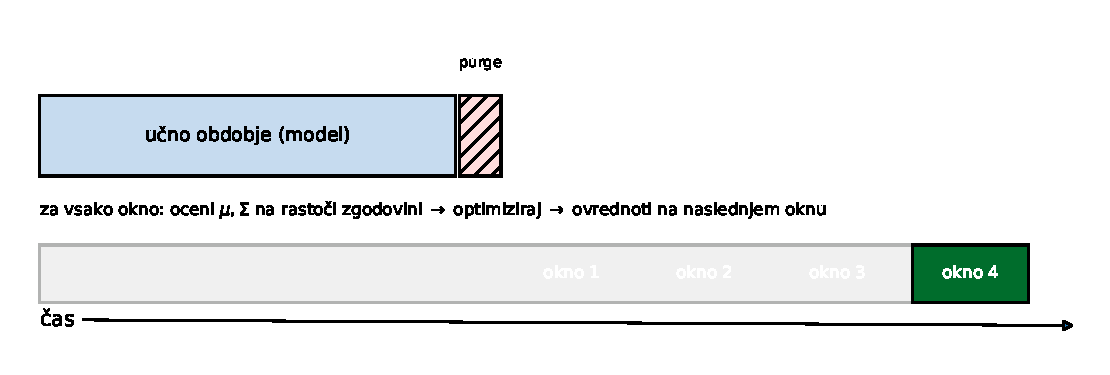
\includegraphics[width=0.92\linewidth]{primer_walkforward}
  \caption{Postopno (walk-forward) vrednotenje: učno obdobje, vrzel (purge) in zaporedna testna okna. Za vsako okno se uporabi le zgodovina do njegovega začetka.}
  \label{fig:pr-wf}
\end{figure}

\paragraph{Transakcijski stroški.} Donose ovrednotimo \emph{neto} po transakcijskih stroških: ob vsakem rebalansiranju od donosa odštejemo strošek, sorazmeren obratu portfelja (spremembi uteži), po stopnji~$10$~bazičnih točk na enoto obrata. Boljša uspešnost napovednega scenarija pride po ceni višjega obrata; poročamo neto Sharpov količnik, ki ta strošek že upošteva.

\paragraph{Statistična značilnost.}\label{sec:stat}
Ker ima posamezen režim malo oken in zato malo statistične moči, značilnost ovrednotimo z \emph{združevanjem} oken čez več režimov ($n\approx 254$) in več robustnih testov.

\paragraph{Signalna raven.} Za vsak vir~$\vec{\mu}$ zberemo IK po oknih čez vse režime in preverimo, ali je povprečni IK značilno pozitiven, z Newey-West popravkom~\cite{neweywest1987} za avtokorelacijo ter s po režimu grupirano~$t$-statistiko (vsak režim kot ena grozd-enota).

\paragraph{Portfeljska raven.} Razliko kumulativnega donosa po oknih med transformerjem in vsako referenco testiramo s parnim~$t$-testom in neparametričnim Wilcoxonovim testom~\cite{demiguel2009}. Ker so mesečna neprekrivajoča okna približno neodvisna, je ta test dobro-močen; po režimu grupiran test poročamo kot najbolj konservativen.

\paragraph{Razlika Sharpovih količnikov.} Razliko anualiziranih Sharpovih količnikov na zloženih dnevnih donosih testiramo z metodo Ledoit-Wolf/Memmel~\cite{ledoitwolf2008,memmel2003} (Newey-West HAC) in stacionarnim samovzorčenjem (angl.\ \emph{bootstrap})~\cite{politis1994}.

\paragraph{Popravek na izbiro.} Ker smo preizkusili več različic strategij, uporabimo \emph{na izbiro popravljeni} Sharpov količnik (PSK; angl.\ \emph{deflated Sharpe ratio})~\cite{baileylopez2014}, ki oceni pričakovani največji Sharpe pod ničelno hipotezo čez vse preizkušene strategije in izračuna verjetnost, da je pravi Sharpe pozitiven kljub temu popravku.

\paragraph{Popravek za mnogotere teze.} Vse parne~$p$-vrednosti dodatno popravimo po postopku Benjamini-Hochberg~\cite{benjamini1995}, ki nadzoruje delež lažnih odkritij pri hkratnem preizkušanju več hipotez.

\section{Neodvisno vrednotenje optimizatorjev}
\label{sec:orlib}

Preden ovrednotimo celoten cevovod, metahevristike neodvisno preverimo na standardnih primerih iz knjižnice OR-Library~\cite{chang2000,beasley1990}. Vsak primer vsebuje priloženo \emph{neomejeno} učinkovito fronto; kakovost hevristike merimo s standardno odstotno napako po Changu in sod.: za vsako točko omejene fronte izračunamo najmanjšo relativno razdaljo do reference. Tabela~\ref{tab:orlib} povzame napako na dveh primerih. Na manjši univerzi (Hang Seng,~$N=31$) se vsi algoritmi približajo objavljeni fronti na okoli en odstotek, kar potrjuje pravilnost implementacije; na večji (DAX~100,~$N=85$) napake pričakovano narastejo. Najbolj robustna sta rojenje delcev in genetski algoritem. Ta preizkus je neodvisen od napovednega dela in preverja izključno kakovost optimizatorjev.

\begin{table}[htbp]
  \centering
  \caption{Standardna odstotna napaka fronte glede na objavljeno neomejeno fronto OR-Library, pri~$K=10$ (nižje je bolje).}
  \label{tab:orlib}
  \begin{tabular}{lcccc}
    \toprule
     & \multicolumn{2}{c}{Hang Seng ($N{=}31$)} & \multicolumn{2}{c}{DAX 100 ($N{=}85$)}\\
    Algoritem & povpr. & mediana & povpr. & mediana\\
    \midrule
    RD         & 1{,}24 & 1{,}34 & 2{,}99 & 2{,}82\\
    SO          & 2{,}70 & 1{,}56 & 3{,}43 & 2{,}90\\
    GA          & 1{,}46 & 1{,}51 & 3{,}97 & 3{,}46\\
    \bottomrule
  \end{tabular}
\end{table}

Sliki~\ref{fig:orlib} to skladnost ponazorita še vizualno: kardinalno omejene fronte vseh treh metahevristik ležijo praktično na objavljeni neomejeni fronti OR-Library, kar potrjuje, da je optimalnostna vrzel zanemarljiva.

\begin{figure}[htbp]
  \centering
  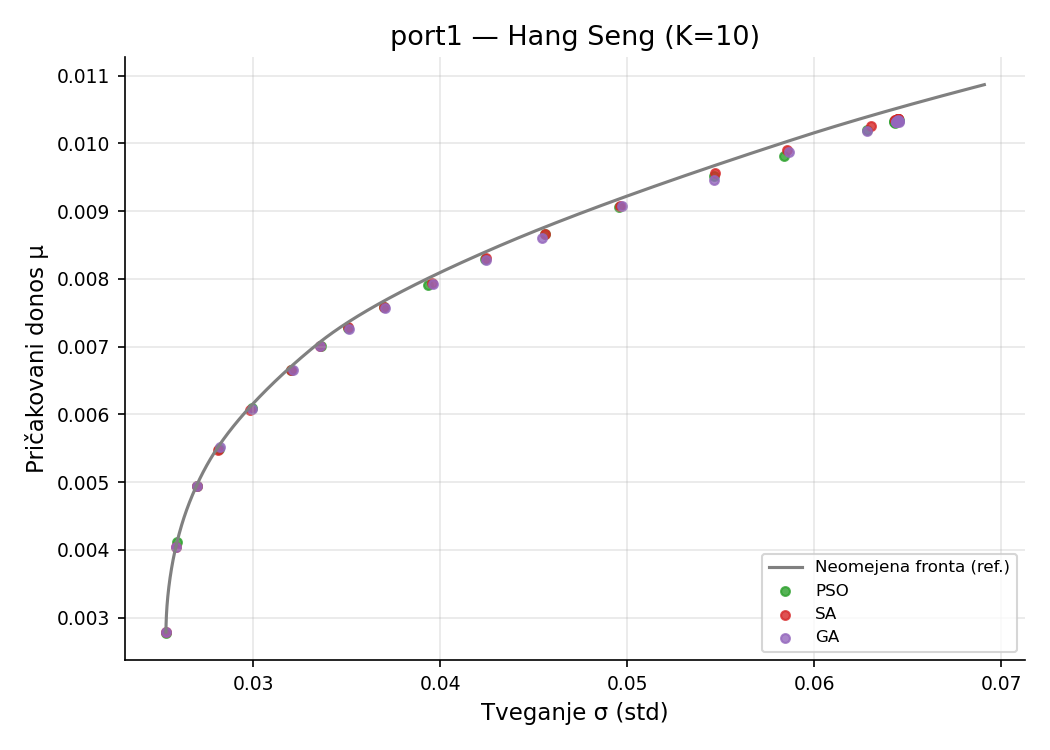
\includegraphics[width=0.49\linewidth]{orlib_frontier_port1}\hfill
  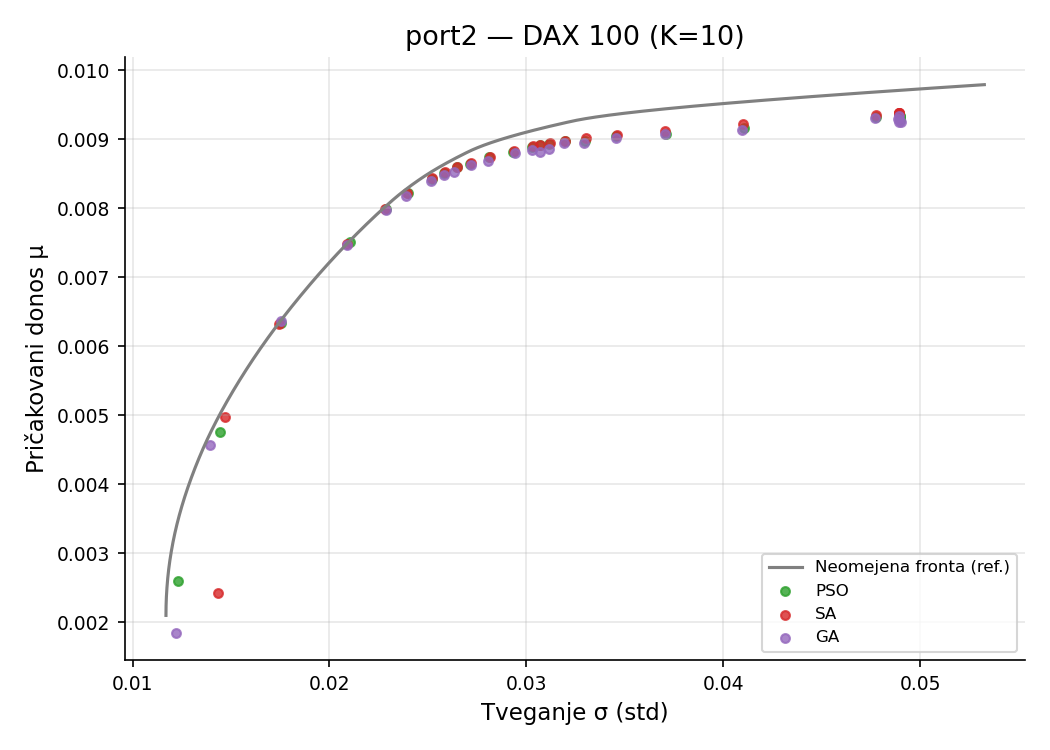
\includegraphics[width=0.49\linewidth]{orlib_frontier_port2}
  \caption{Kardinalno omejene fronte metahevristik na primerih Hang Seng (levo) in DAX 100 (desno) proti objavljeni neomejeni fronti OR-Library (siva krivulja). Vsaka točka je rešitev pri eni vrednosti~$\lambda$; RD (zelena), SO (rdeča) in GA (vijolična) se skoraj popolnoma prekrivajo in ležijo tik ob referenčni fronti.}
  \label{fig:orlib}
\end{figure}

\section{Napovedna kakovost in robustnost čez režime}
\label{sec:setup}

Celoten cevovod testiramo na univerzah ameriških delnic velike kapitalizacije, s kardinalnostjo~$K=10$, mejama uteži~$\varepsilon=0{,}02$ in~$\delta=0{,}30$, osnovnim parametrom tveganja~$P=0{,}8$ in transakcijskimi stroški~$10$~bazičnih točk. Da bi ocenili robustnost skozi različne razmere, poskus ponovimo v \emph{šestih tržnih režimih}: dveh krizah (globalna finančna kriza 2007--2010 in pandemija 2019--2021), umirjenem obdobju z vračanjem k sredini (2013--2017), obdobju dvigovanja obrestnih mer (2022--2024) ter dveh različicah obdobja 2019--2022 --- s tehnološkimi velikani (\emph{headline}) in brez njih (\emph{divuniverse}). Skupno čez vse režime dobimo~$n\approx 254$ zaporednih neprekrivajočih oken.

\paragraph{Kakovost napovedi.}\label{sec:ic}
Osrednji nadzorni pokazatelj je informacijski koeficient (IK). Ko IK združimo čez vse režime, je transformer \emph{edini} vir napovedi z opazno pozitivno zunaj-vzorčno napovedno močjo (povprečni IK~$+0{,}027$; po režimu grupirana~$t$-statistika~$2{,}22$,~$p\approx 0{,}077$), medtem ko so vse reference praktično nič ali negativne: zgodovinsko povprečje~$-0{,}019$, BL~$-0{,}018$, gradientni gozd~$-0{,}004$, LSTM~$+0{,}004$ (neznačilno). Transformer se torej kot signal loči od vseh preizkušenih alternativ.

\paragraph{Robustnost čez režime.}\label{sec:regimes}
Tabela~\ref{tab:regimes} prikazuje Sharpov količnik po posameznih režimih. Transformerski cevovod prekaša klasično zgodovinsko referenco v \emph{petih od šestih} režimih; edina izjema je okrevanje po pandemiji (COVID 2020), izrazito obdobje vračanja k sredini, kjer drseče zgodovinsko povprečje prednjači. Prednost je največja prav v krizi 2008, kjer klasična referenca izgublja (Sharpe~$0{,}14$), transformer pa doseže~$0{,}73$. Poučen je kontrast med \emph{headline} in \emph{divuniverse}: brez tehnoloških velikanov se prednost transformerja ne zmanjša, temveč \emph{poveča} (Sharpe~$1{,}27$ proti~$0{,}28$), kar ovrže pomislek, da gre le za statično stavo na peščico velikanov. Slika~\ref{fig:regimegrid} to prikaže še vizualno.

\begin{table}[htbp]
  \centering
  \caption{Sharpov količnik (algoritem RD, na zloženih dnevnih donosih) po tržnih režimih; zadnji stolpec je predznak združenega IK transformerja. Transformer prekaša zgodovinsko referenco v petih od šestih režimov (izjema COVID).}
  \label{tab:regimes}
  \begin{tabular}{lrrrc}
    \toprule
    Režim & Transformer & Zgodovinski & LSTM & IK transf.\\
    \midrule
    divuniverse (2019--22, brez velikanov) & 1{,}27 & 0{,}28 & 0{,}73 & $+$\\
    GFC (kriza 2008)                       & 0{,}73 & 0{,}14 & 0{,}13 & $+$\\
    COVID (kriza 2020)                     & 1{,}06 & 1{,}73 & 1{,}03 & $-$\\
    2013--2017 (umirjen trg)               & 1{,}96 & 1{,}34 & 0{,}99 & $+$\\
    2022--2024 (dvig obr.\ mer)            & 1{,}04 & 0{,}47 & 1{,}09 & $+$\\
    headline (2019--22, z velikani)        & 0{,}43 & 0{,}43 & 0{,}62 & $+$\\
    \bottomrule
  \end{tabular}
\end{table}

Da sliko dopolnimo z absolutnimi donosi, Tabela~\ref{tab:regimescum} prikazuje končni kumulativni donos (neto, algoritem RD) treh scenarijev in dveh naivnih referenc po režimih. Prednost transformerja je izrazita v krizi 2008 (kjer zgodovinski izgublja) in v razpršenem univerzumu \emph{divuniverse} ($+197\,\%$ proti~$+16\,\%$), medtem ko v okrevanju po pandemiji zaostane. Ansambel v vsakem režimu sledi boljšemu ekspertu: kjer transformer zmaga, ga posnema (ali celo prekaša, npr.\ GFC in 2022), kjer pa zaostane (COVID), se nasloni na zgodovinskega ($+229\,\%$ proti transformerjevim~$+125\,\%$).

\begin{table}[htbp]
  \centering
  \caption{Končni kumulativni donos (\%) po režimih (algoritem RD, neto po stroških): transformer (T), zgodovinski (Z), ansambel (A) ter naivni referenci~$1/N$ in tržni indeks (Trg).}
  \label{tab:regimescum}
  \begin{tabular}{lrrrrr}
    \toprule
    Režim & T & Z & A & $1/N$ & Trg\\
    \midrule
    2013--2017 (umirjen trg)      & $+630$ & $+258$ & $+550$ & $+133$ & $+81$\\
    GFC (kriza 2008)              & $+145$ & $-8$   & $+151$ & $+26$  & $-3$\\
    COVID (kriza 2020)            & $+125$ & $+244$ & $+229$ & $+107$ & $+86$\\
    2022--2024 (dvig obr.\ mer)   & $+92$  & $+29$  & $+100$ & $+41$  & $+29$\\
    divuniverse (brez velikanov)  & $+197$ & $+16$  & $+183$ & $+50$  & $+31$\\
    headline (z velikani)         & $+42$  & $+39$  & $+28$  & $+60$  & $+31$\\
    \bottomrule
  \end{tabular}
\end{table}

\begin{figure}[htbp]
  \centering
  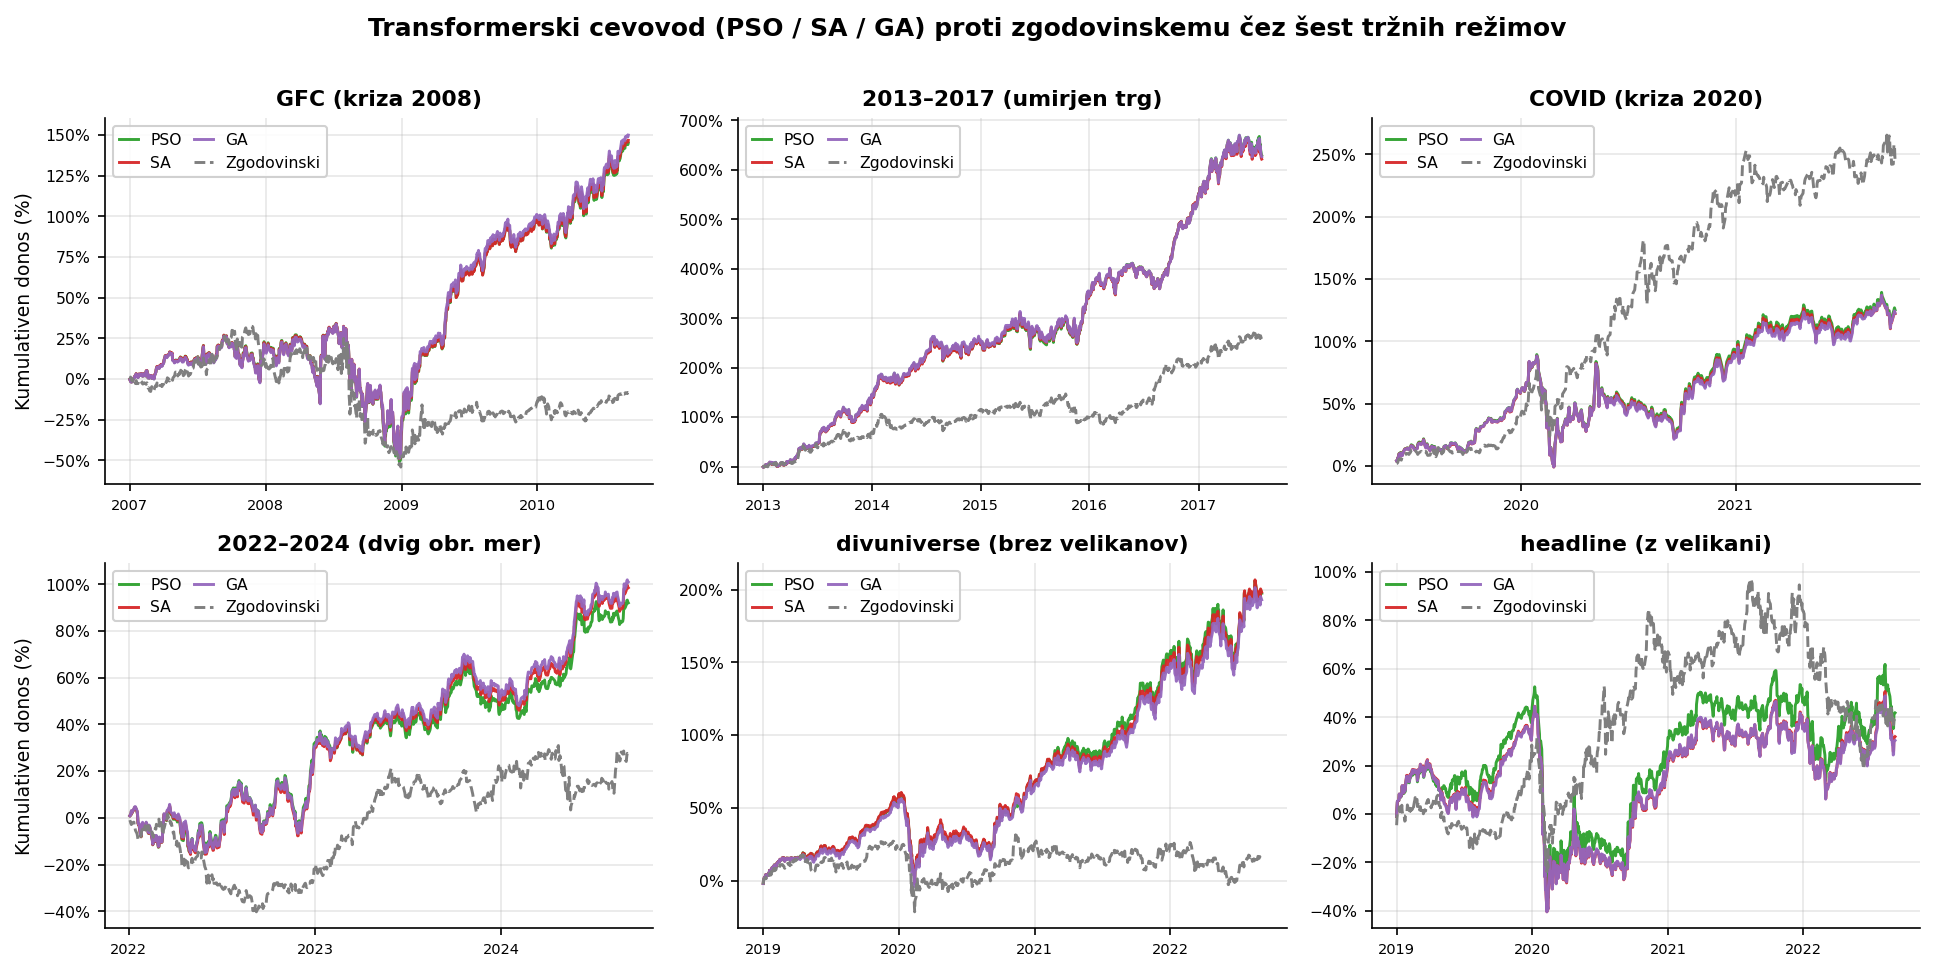
\includegraphics[width=\linewidth]{regime_grid_algos}
  \caption{Kumulativni donos transformerskega cevovoda čez vseh šest režimov. V vsakem panelu so posamezne metahevristike RD/SO/GA, kot referenca pa klasični zgodovinski cevovod (siva črtkana). Znotraj vsakega režima se solverji tesno ujemajo; razlike med paneli izvirajo iz napovednega signala in tržnega režima.}
  \label{fig:regimegrid}
\end{figure}

\section{Združeni preizkus in zunanja veljavnost}
\label{sec:pooled}

Osrednji rezultat dobimo z združevanjem vseh~$n\approx 254$ oken (Tabela~\ref{tab:pooled}). Transformerski cevovod doseže letni Sharpov količnik~$0{,}97$ (ansambel~$1{,}01$), bistveno več kot vse reference (zgodovinski~$0{,}64$, BL~$0{,}58$, LSTM~$0{,}58$, gradientni gozd~$0{,}35$). Prednost je značilna po večih merilih: razlika kumulativnega donosa po oknih je za gradientni gozd in LSTM značilna pri~$p<0{,}01$ ter za BL in zgodovinski cevovod pri~$p<0{,}05$; test razlike Sharpovih količnikov~\cite{ledoitwolf2008,memmel2003} to potrdi ($\Delta$SK do~$+0{,}62$,~$p<0{,}001$); vseh~$12$~parnih testov prestane popravek Benjamini-Hochberg~\cite{benjamini1995}. Najbolj prepričljiv je na izbiro popravljeni Sharpov količnik~\cite{baileylopez2014}: ostaneta značilno pozitivna \emph{le} transformer (PSK~$0{,}994$) in ansambel ($0{,}996$), medtem ko \emph{vse} reference tej korekciji podležejo.

\begin{table}[htbp]
  \centering
  \caption{Združeni rezultati čez vseh šest režimov ($n\approx 254$ oken). Parni preizkusi glede na transformer: razlika kum.\ donosa na okno ($\Delta$don.), njena~$p$-vrednost, razlika letnega Sharpa ($\Delta$SK) in na izbiro popravljeni Sharpov količnik (PSK).}
  \label{tab:pooled}
  \begin{tabular}{lrrrrr}
    \toprule
    Strategija & Sharpe & $\Delta$don.\% & $p$ & $\Delta$SK & PSK\\
    \midrule
    Transformer      & 0{,}97 & ---   & ---     & ---    & 0{,}994\\
    Ansambel         & 1{,}01 & ---   & ---     & ---    & 0{,}996\\
    Zgodovinski      & 0{,}64 & $+1{,}22$ & 0{,}031 & $+0{,}33$ & 0{,}834\\
    Black-Litterman  & 0{,}58 & $+1{,}38$ & 0{,}023 & $+0{,}39$ & 0{,}762\\
    LSTM             & 0{,}58 & $+1{,}26$ & 0{,}001 & $+0{,}39$ & 0{,}762\\
    Gradientni gozd  & 0{,}35 & $+2{,}03$ & $<0{,}001$ & $+0{,}62$ & 0{,}360\\
    \bottomrule
  \end{tabular}
\end{table}

Poleg Sharpovega količnika Tabela~\ref{tab:pooledrisk} podaja še dodatne mere tveganja na združenih dnevnih donosih. Transformer in ansambel prekašata zgodovinski scenarij po vseh merilih: višji Sortinov količnik (boljše razmerje do negativne volatilnosti) in višje razmerje Omega, ob primerljivi volatilnosti in največjem upadu. Visok največji upad ($\sim\!60\,\%$) pri vseh scenarijih izvira iz vključenih kriznih režimov (2008, 2020).

\begin{table}[htbp]
  \centering
  \caption{Dodatne mere uspešnosti in tveganja na združenih dnevnih donosih (algoritem RD, čez vseh šest režimov): letni Sharpov in Sortinov količnik, razmerje Omega, največji upad in letna volatilnost.}
  \label{tab:pooledrisk}
  \begin{tabular}{lrrrrr}
    \toprule
    Scenarij & Sharpe & Sortino & Omega & Max.\ upad (\%) & Volatilnost (\%)\\
    \midrule
    Transformer & 0{,}97 & 1{,}30 & 1{,}21 & 63 & 34\\
    Ansambel    & 1{,}01 & 1{,}30 & 1{,}22 & 62 & 33\\
    Zgodovinski & 0{,}64 & 0{,}82 & 1{,}13 & 65 & 30\\
    \bottomrule
  \end{tabular}
\end{table}

\paragraph{Poštena omejitev in vloga ansambla.} Prednost pred \emph{golim zgodovinskim povprečjem} ostaja ekonomsko smiselna, a statistično mejna ($\Delta$don.~$+1{,}2\,\%$ na okno;~$\Delta$SK~$+0{,}33$,~$p\approx 0{,}07$); to je pošteno predstaviti kot mejno in ne kot dokazano prednost. Prav zato je vloga ansambla v robustnosti. To se najbolje pokaže v edinem režimu, kjer transformer zaostane za zgodovinskim --- pri okrevanju po pandemiji (Slika~\ref{fig:ensadv}): transformer tam doseže le~$+125\,\%$, ansambel Hedge pa sledi zmagovalnemu zgodovinskemu ekspertu in ostane pri~$+229\,\%$ (zgodovinski~$+244\,\%$), namesto da bi se sesul na raven transformerja. To je neposredna ponazoritev meje regreta: kombinacija ne sledi izgubljajočemu viru navzdol, temveč ostane ob najboljšem. V režimih, kjer transformer zmaga (npr.\ kriza 2008 in obdobje 2022), ansambel celo \emph{prekaša oba} eksperta (Slika~\ref{fig:walkforward}).

\begin{figure}[htbp]
  \centering
  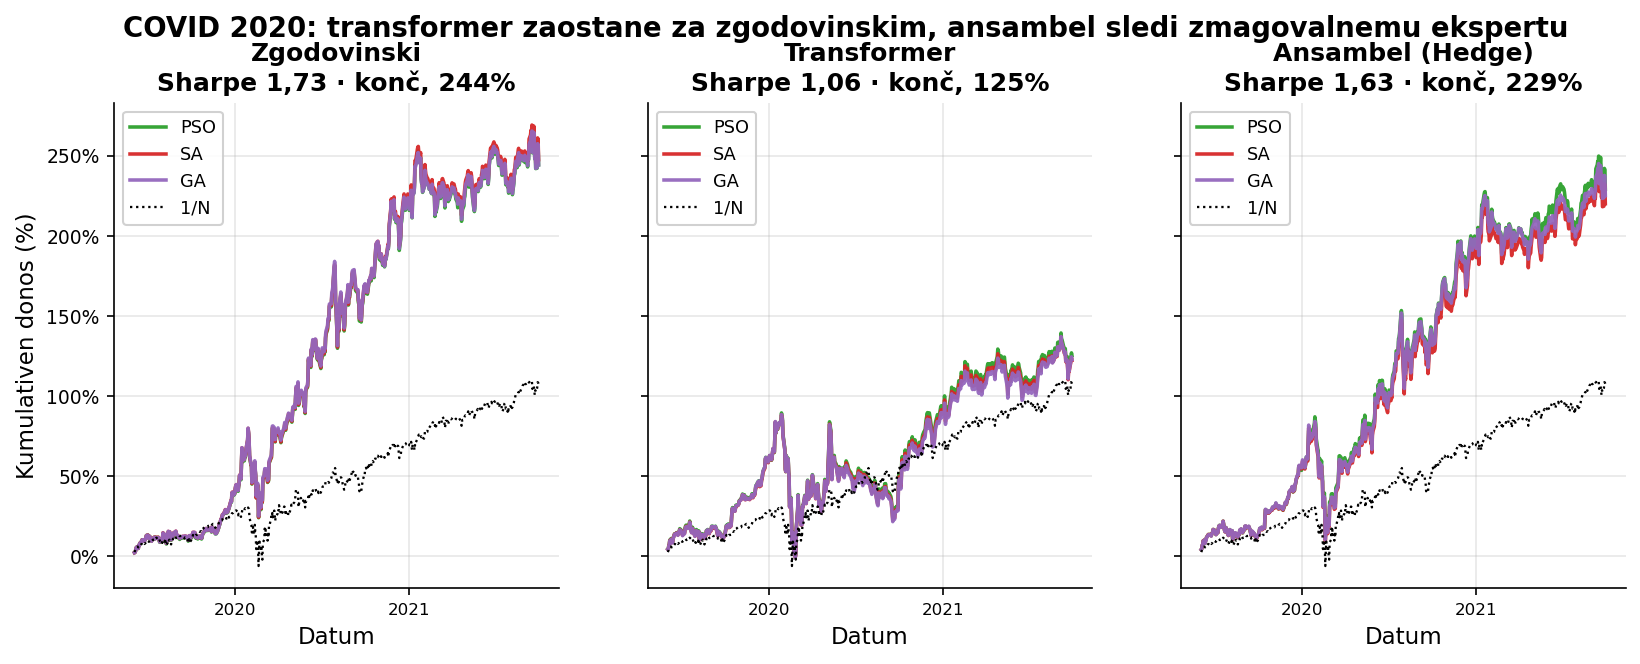
\includegraphics[width=\linewidth]{ensemble_advantage_covid}
  \caption{Robustnost ansambla v edinem režimu, kjer transformer zaostane za zgodovinskim --- okrevanje po pandemiji (COVID 2020). Ansambel Hedge sledi zmagovalnemu zgodovinskemu ekspertu ($+229\,\%$ proti transformerjevim~$+125\,\%$), namesto da bi se sesul na raven transformerja.}
  \label{fig:ensadv}
\end{figure}

\begin{figure}[htbp]
  \centering
  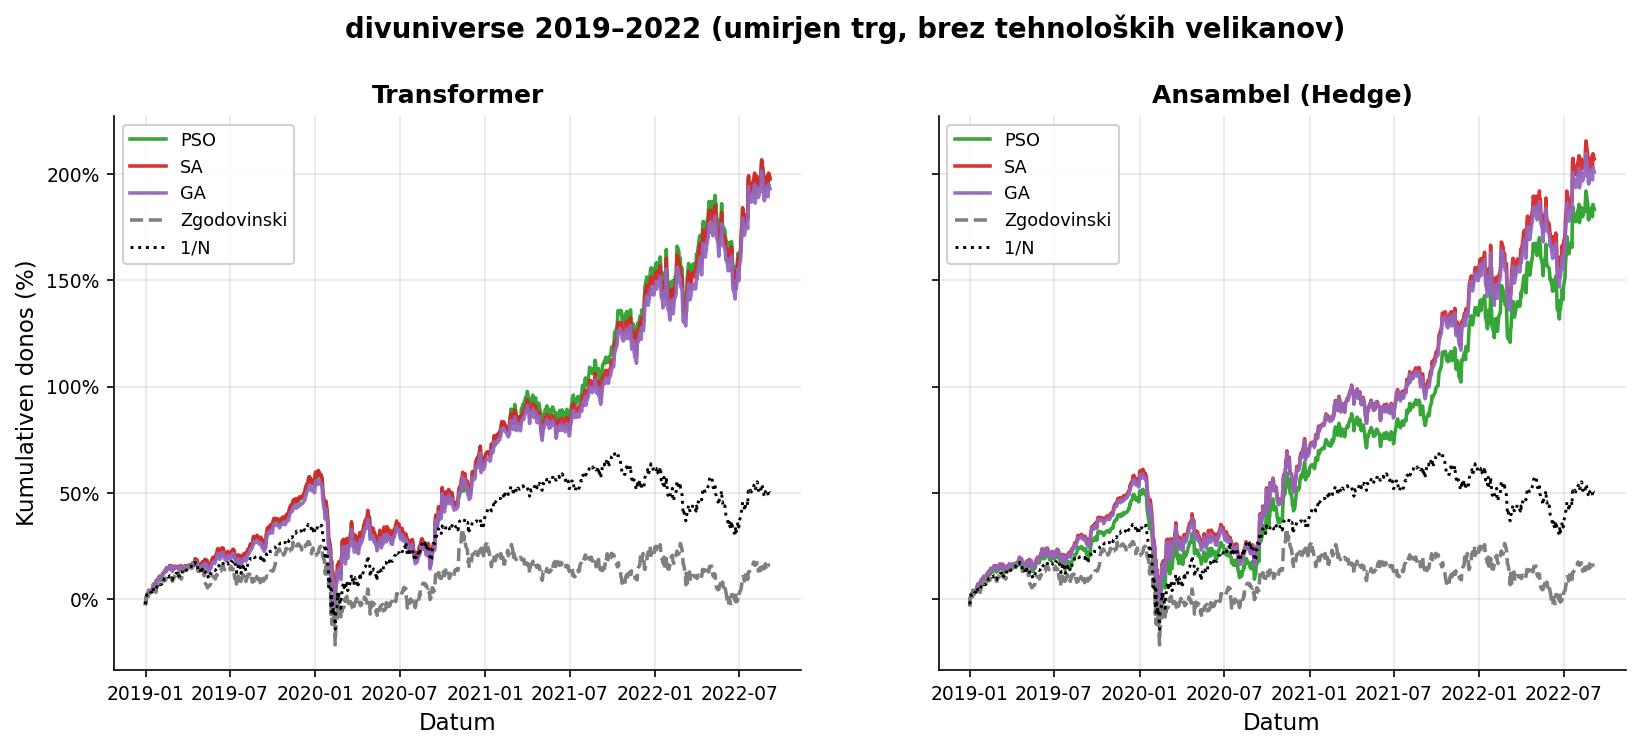
\includegraphics[width=\linewidth]{walkforward_divuniverse_panels}\\[2pt]
  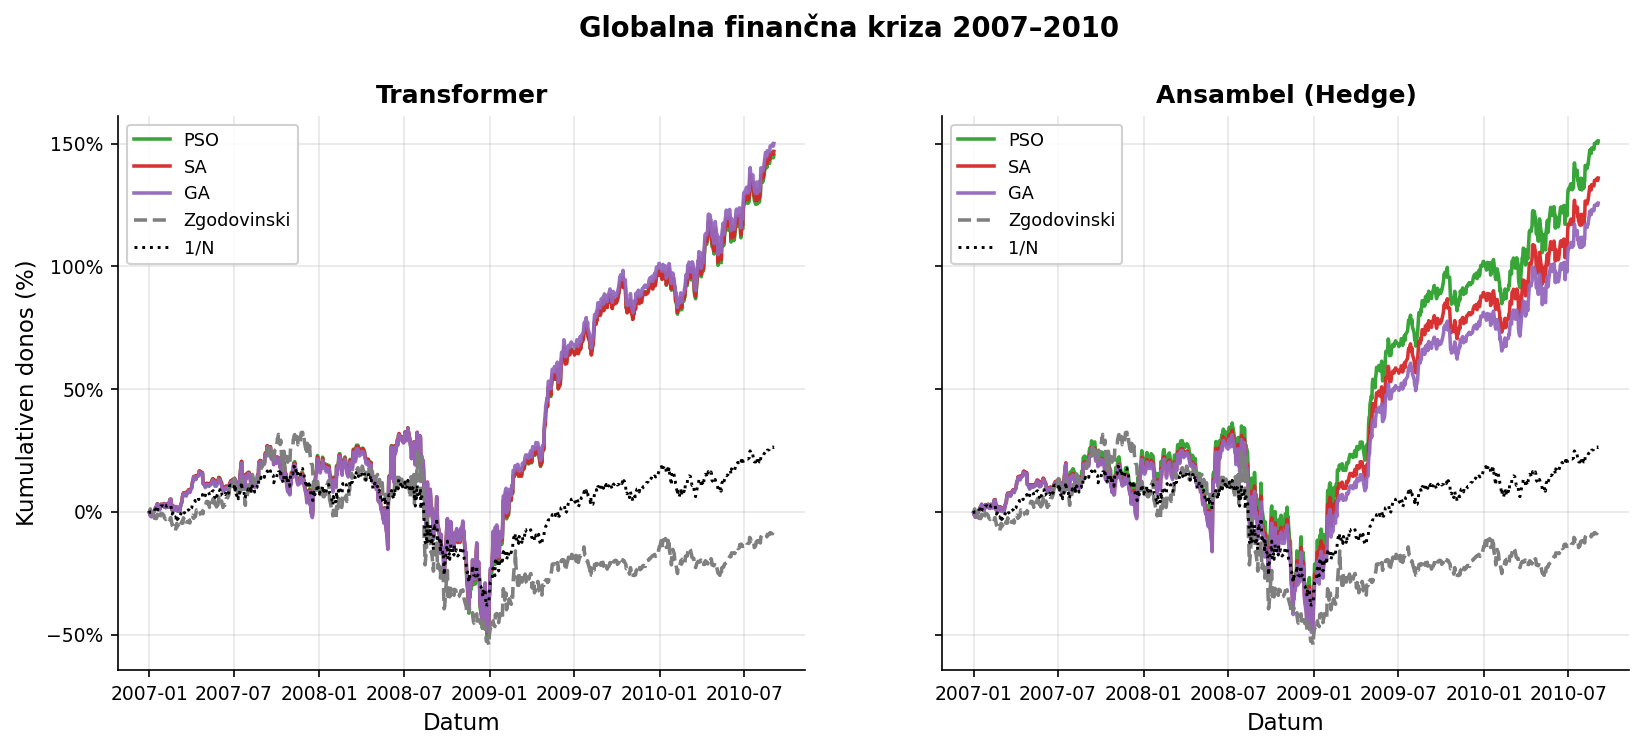
\includegraphics[width=\linewidth]{walkforward_gfc_panels}
  \caption{Kumulativni donos vseh treh metahevristik v dveh nasprotnih režimih: umirjeno obdobje \emph{divuniverse} (zgoraj) in kriza 2008 (spodaj). Vse tri metahevristike se tesno ujemajo in opazno prekašajo klasični cevovod ter~$1/N$; prednost je najizrazitejša v krizi.}
  \label{fig:walkforward}
\end{figure}

\paragraph{Neposredni primerjavi na tujem protokolu.}\label{sec:headtohead}
Da se izognemo očitku, da so rezultati odvisni od naše izbire režimov, cevovod poženemo tudi na protokolu dveh objavljenih študij. (i)~Na protokolu Ramos in sod.~\cite{ramos2023} (S\&P~100, 2011--2021, kardinalna omejitev do~$20$ sredstev, drseče okno, $30$~bazičnih točk) naš transformerski cevovod doseže letni Sharpov količnik~$1{,}11$ (ansambel~$1{,}07$), kar preseže njihovo objavljeno referenco indeksa S\&P~100 ($0{,}99$). (ii)~Na protokolu Fernandes in Desell~\cite{fernandes2026} ($50$~delnic S\&P~500, 2022--2023, četrtletno rebalansiranje, stroški) naš cevovod doseže Sharpe~$0{,}77$ proti njihovemu najboljšemu modelu (AttentionLSTM,~$0{,}29$), in to ob \emph{strožji} kardinalni omejitvi ($K{=}10$). Ker se univerzumi, ciljne funkcije in omejitve ne ujemajo popolnoma, sta primerjavi na ravni protokola in metrike, a obe kažeta v isto smer.

\section{Testiranje po posameznih režimih}
\label{sec:perregime}

V tem razdelku za vsak testni režim (in za obe neposredni primerjavi na tujem protokolu) podamo podrobno razlago tržnih razmer in komentar rezultatov, skupaj s tremi slikami postopnega vrednotenja na eni strani: (i)~kumulativni donos vseh treh scenarijev za vsako metahevristiko (RD/SO/GA) posebej, (ii)~zbirni prikaz kumulativnega donosa reprezentativnega solverja (RD) z referenčnimi strategijami ter (iii)~sestava portfelja skozi čas. Pri slednji je za preglednost prikazanih le~$12$ najpogosteje izbranih sredstev, ostala pa so združena v postavko ``drugo''; v \emph{vsakem} oknu je zaradi kardinalne omejitve izbranih natanko~$K=10$ sredstev, množica pa se ob mesečnem rebalansiranju spreminja.

\subsection{2013--2017: umirjeno obdobje z vračanjem k sredini}
\label{sec:reg-201301}

Obdobje 2013--2017 je bilo dolgotrajen bikovski trg z nizko volatilnostjo in postopno rastjo ob podpori ohlapne denarne politike. Presečni signali (relativna moč med delnicami) so v takem okolju stabilni, zato je to najugodnejši režim za napovedni model: transformer doseže najvišji Sharpe med vsemi režimi ($1{,}96$ proti zgodovinskim~$1{,}34$; Tabela~\ref{tab:regimes}) in končni donos~$+630\,\%$ proti~$+258\,\%$ (Tabela~\ref{tab:regimescum}). Slika~\ref{fig:reg-201301} kaže, da vse tri metahevristike sledijo skoraj identični poti, transformerski scenarij pa se od zgodovinskega loči že zgodaj in prednost vztrajno veča. Ansambel se tesno drži transformerja ($+550\,\%$), saj Hedge hitro prepozna zmagujočega eksperta. Sestava portfelja je razmeroma stabilna, z zmernim obratom med rebalansiranji.

\begin{figure}[p]
  \centering
  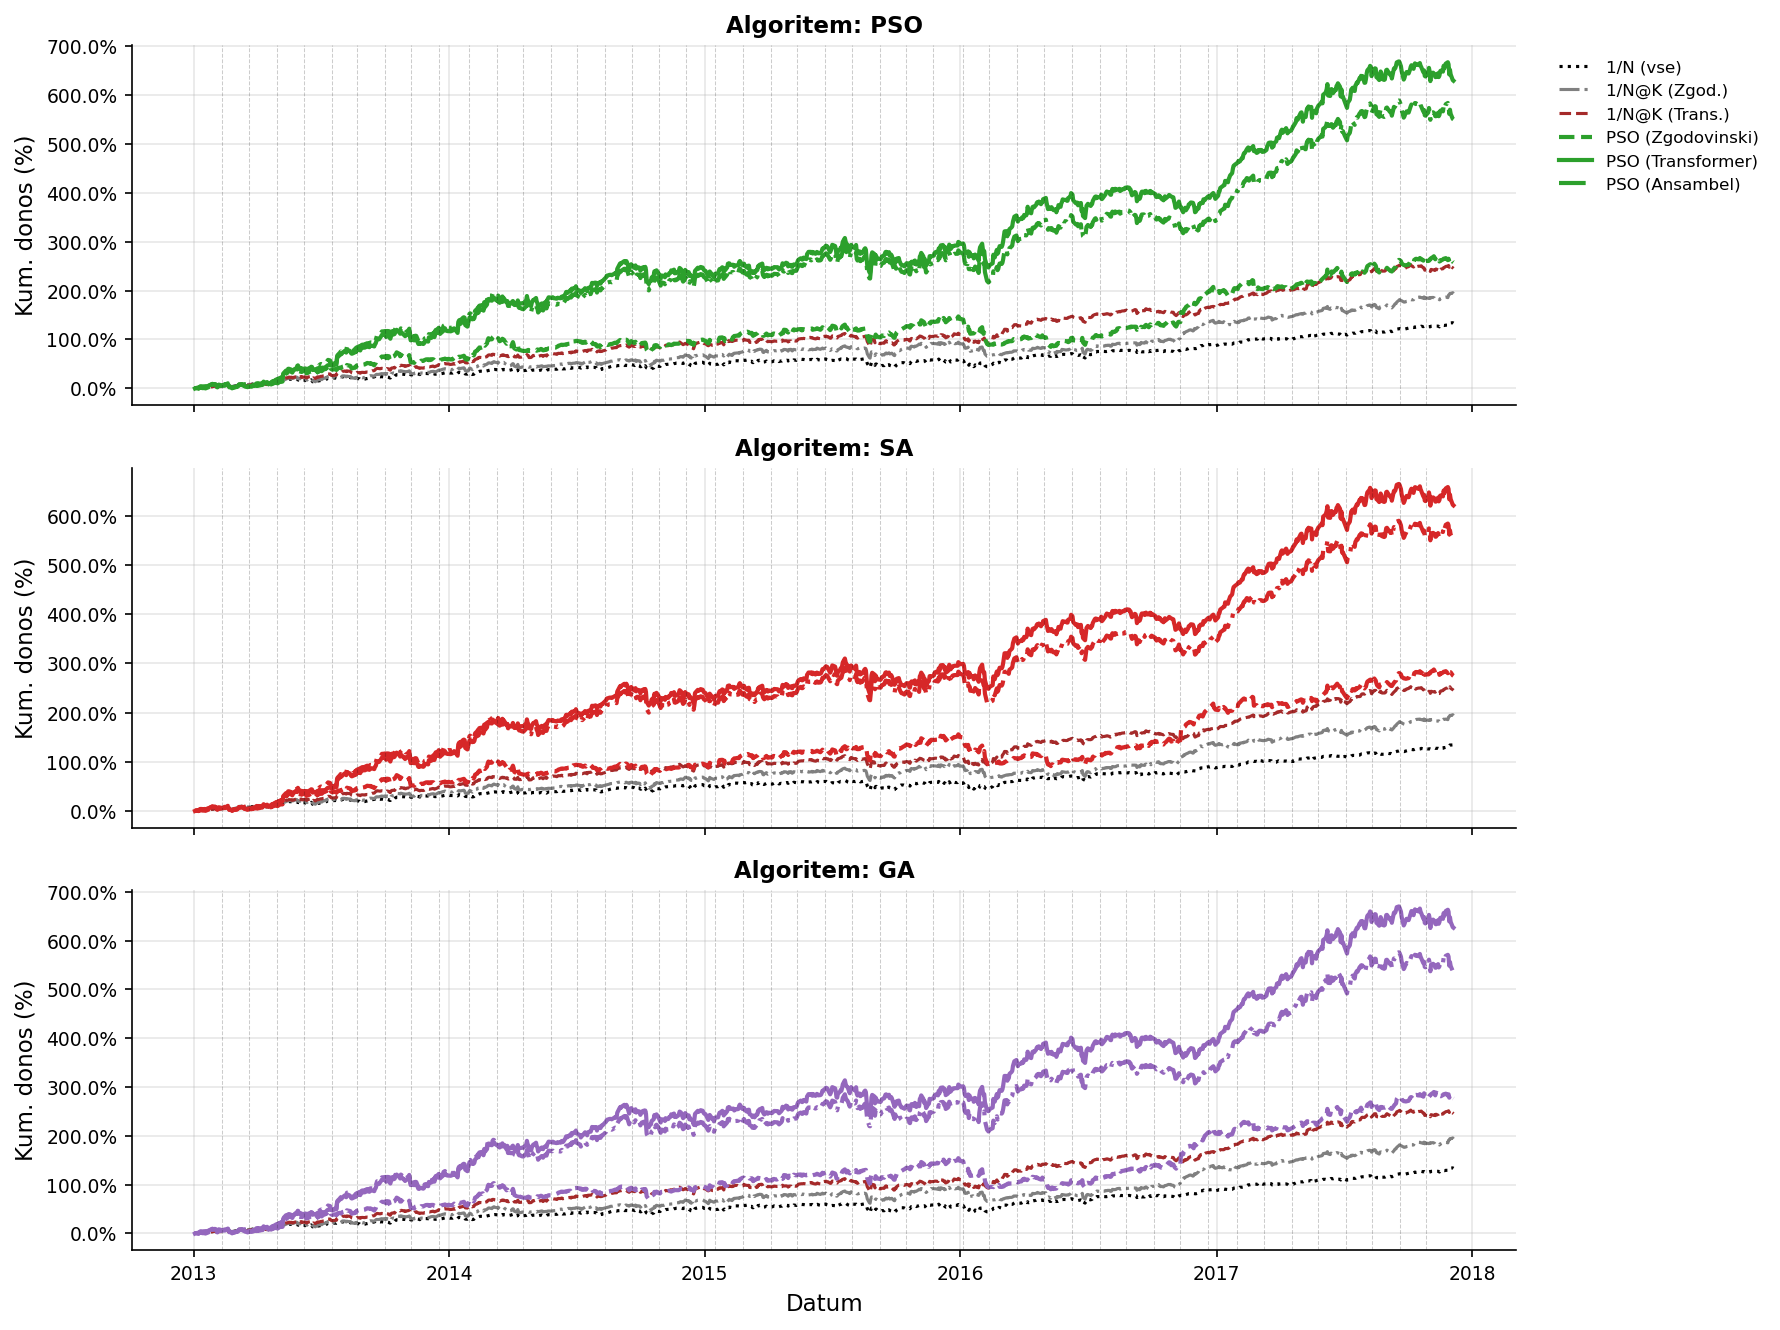
\includegraphics[height=0.30\textheight]{all_algorithms_grid_201301_201712}\\[3pt]
  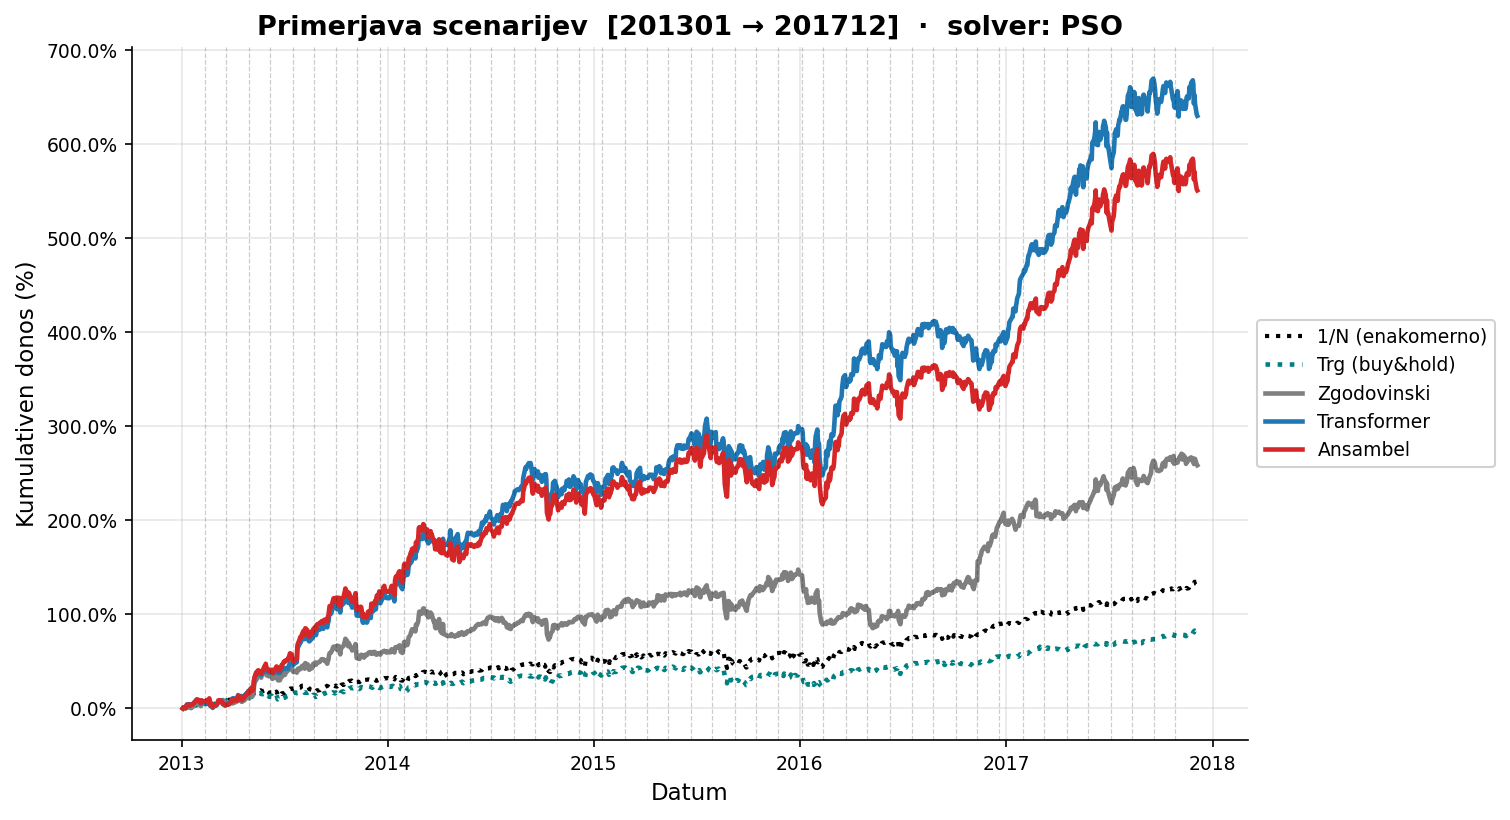
\includegraphics[height=0.30\textheight]{combined_walkforward_201301_201712}\\[3pt]
  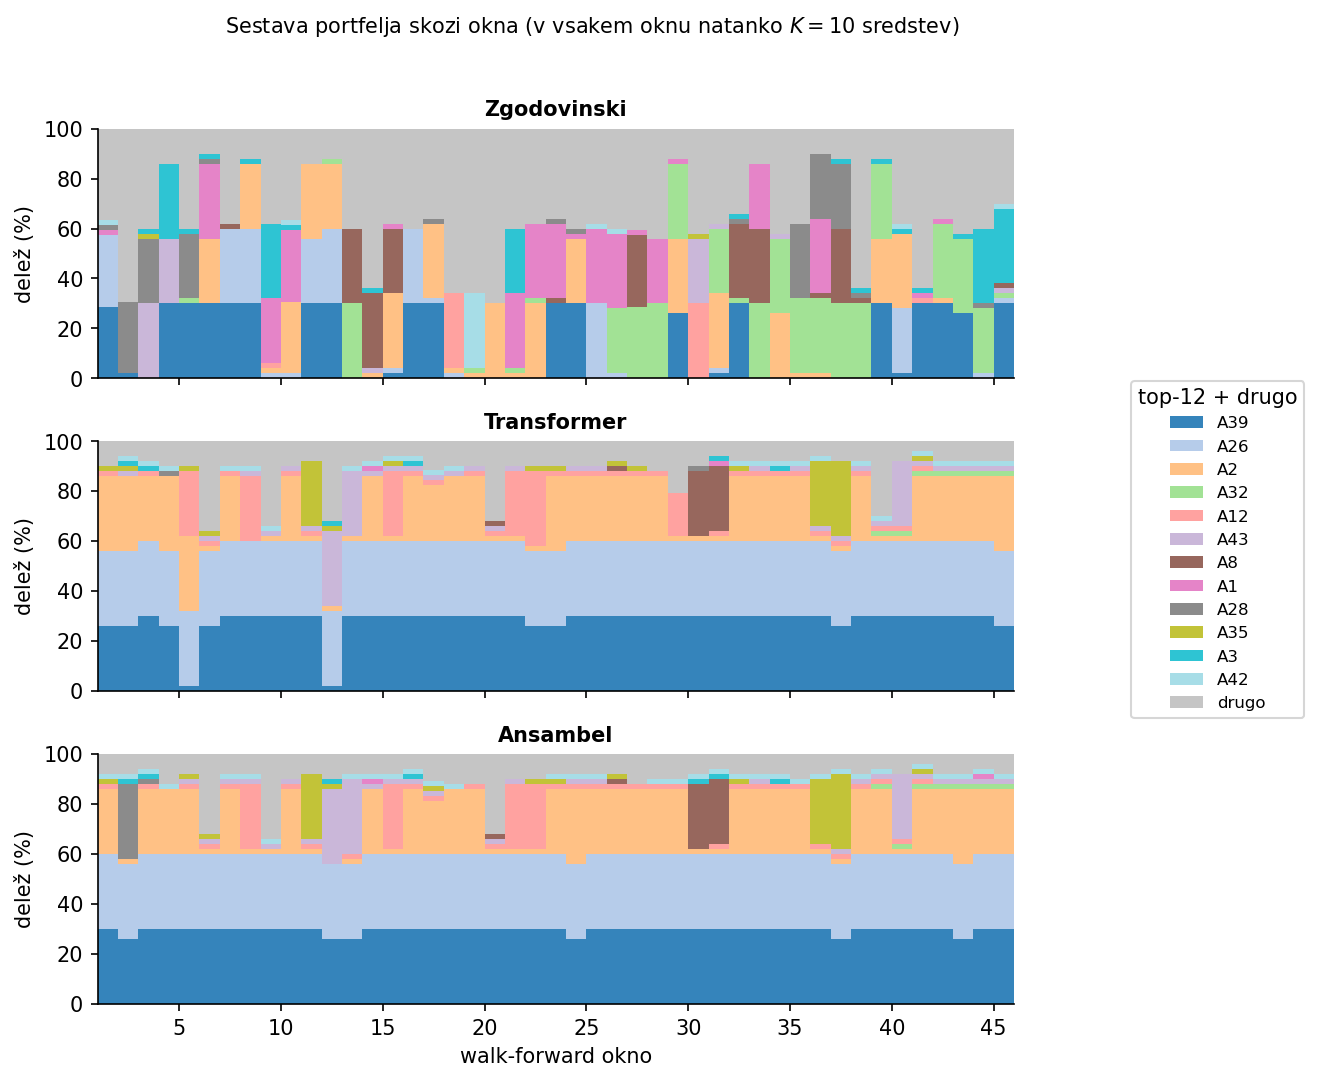
\includegraphics[height=0.26\textheight]{weights_top_201301_201712}
  \caption{Režim 2013--2017 (umirjen trg): (zgoraj) kumulativni donos treh scenarijev za vsako metahevristiko posebej; (sredina) zbirni prikaz s klasičnimi in naivnimi referencami; (spodaj) sestava portfelja skozi walk-forward okna (12 najpogostejših sredstev + ``drugo''; v vsakem oknu natanko~$K=10$ aktivnih).}
  \label{fig:reg-201301}
\end{figure}

\subsection{Globalna finančna kriza 2007--2010}
\label{sec:reg-gfc}

Globalna finančna kriza je najzahtevnejši preizkus: strm sistemski zlom jeseni 2008, sledi mu oster odboj 2009. Klasična zgodovinska ocena~$\vec{\mu}$ zaostaja, ker drseče povprečje počasi reagira na prelom in v padec vstopa s prevelikim tveganjem --- zgodovinski scenarij konča pri~$-8\,\%$ (Sharpe~$0{,}14$). Transformer, ki presečno razvršča relativno moč in prek dinamičnega~$P$~\eqref{eq:dynp} v visoki volatilnosti zmanjša izpostavljenost, se ubrani padca in izkoristi odboj ($+145\,\%$, Sharpe~$0{,}73$) --- to je največja relativna prednost transformerja med vsemi režimi. Ansambel prek Hedge celo rahlo prekaša transformerja ($+151\,\%$). Slika~\ref{fig:reg-gfc} lepo pokaže razhod med scenariji ob zlomu in obvladan upad transformerskega cevovoda; sestava portfelja se ob krizi izraziteje preureja (višji obrat) proti obrambnim sredstvom.

\begin{figure}[p]
  \centering
  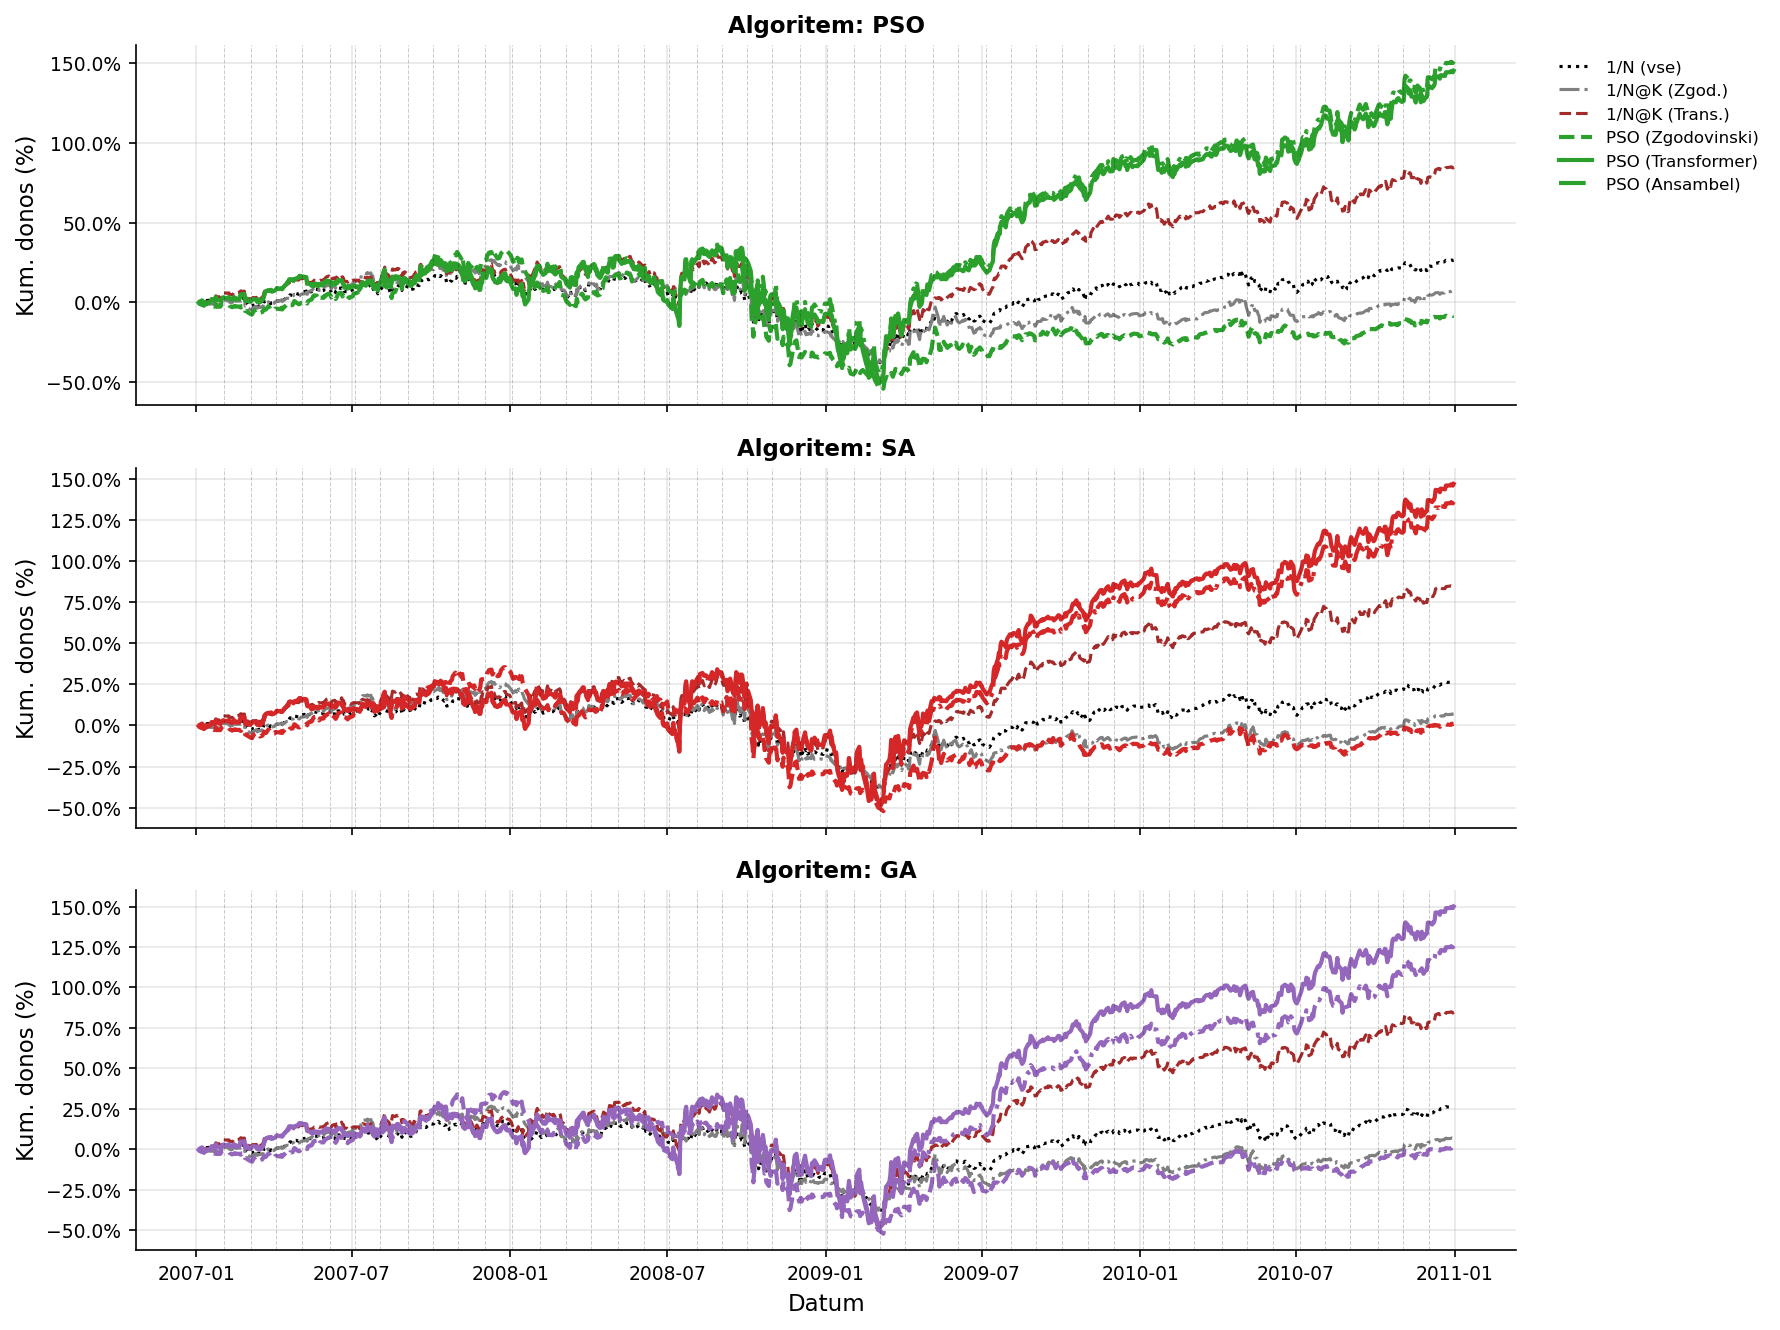
\includegraphics[height=0.30\textheight]{all_algorithms_grid_200701_201012_gfc2008}\\[3pt]
  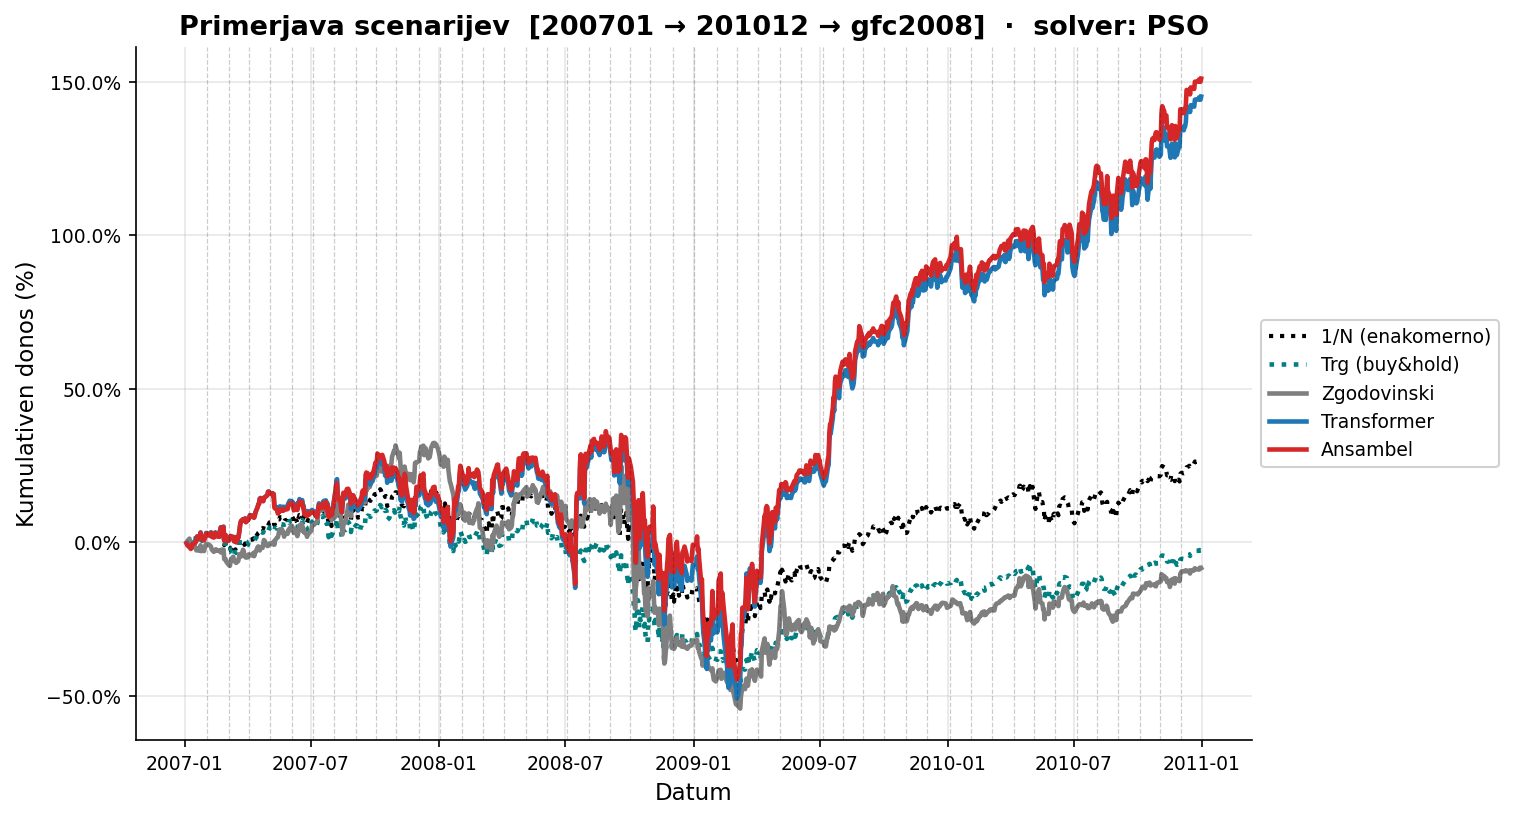
\includegraphics[height=0.30\textheight]{combined_walkforward_200701_201012_gfc2008}\\[3pt]
  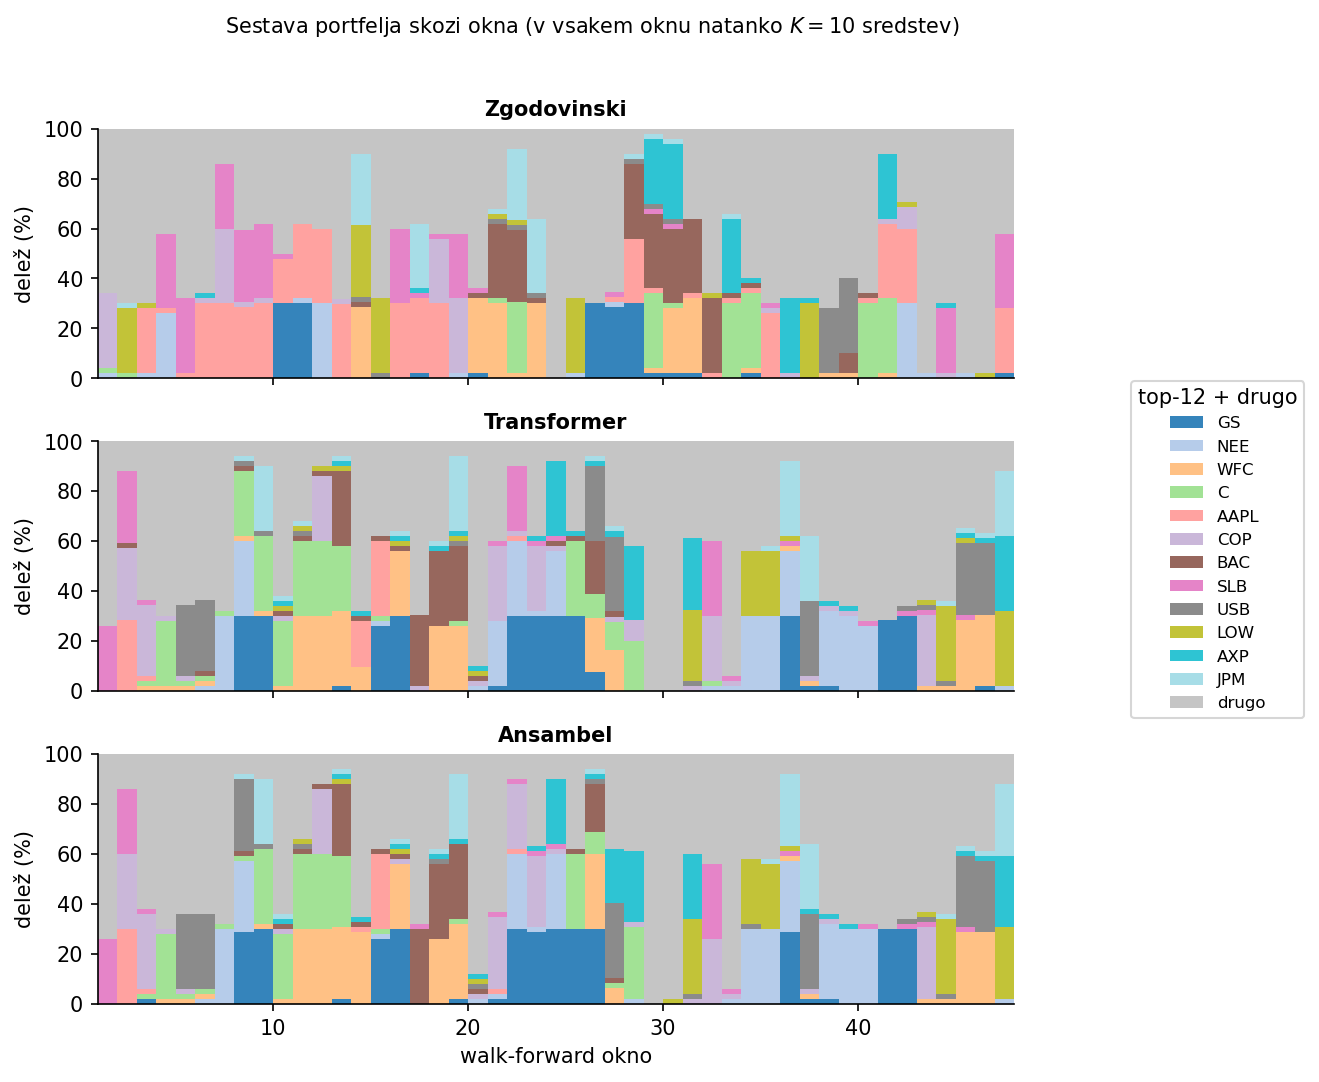
\includegraphics[height=0.26\textheight]{weights_top_200701_201012_gfc2008}
  \caption{Režim globalne finančne krize 2007--2010: (zgoraj) trije scenariji po metahevristikah; (sredina) zbirni prikaz z referencami; (spodaj) sestava portfelja skozi okna (natanko~$K=10$ aktivnih na okno).}
  \label{fig:reg-gfc}
\end{figure}

\subsection{Pandemija COVID 2019--2021}
\label{sec:reg-covid}

Pandemija je edini režim, kjer transformer zaostane za zgodovinsko referenco. Zlom marca 2020 je bil izjemno hiter, sledilo pa mu je še hitrejše, ozko okrevanje (V-oblika), ki ga je poganjala peščica sredstev z močnim vračanjem k sredini. V takem okolju drseče zgodovinsko povprečje, ki teža k nedavnim padcem, ujame prav ta odboj: zgodovinski scenarij doseže Sharpe~$1{,}73$ in~$+244\,\%$, transformer pa~$1{,}06$ in~$+125\,\%$ (Tabeli~\ref{tab:regimes} in~\ref{tab:regimescum}). Tu se pokaže vrednost ansambla: Hedge zazna, da zgodovinski ekspert vodi, in se nasloni nanj ($+229\,\%$), namesto da bi sledil šibkejšemu transformerju (glej tudi Sliko~\ref{fig:ensadv}). Slika~\ref{fig:reg-covid} prikazuje ta razhod in prilagoditev ansambla; portfelj se ob zlomu močno preuredi.

\begin{figure}[p]
  \centering
  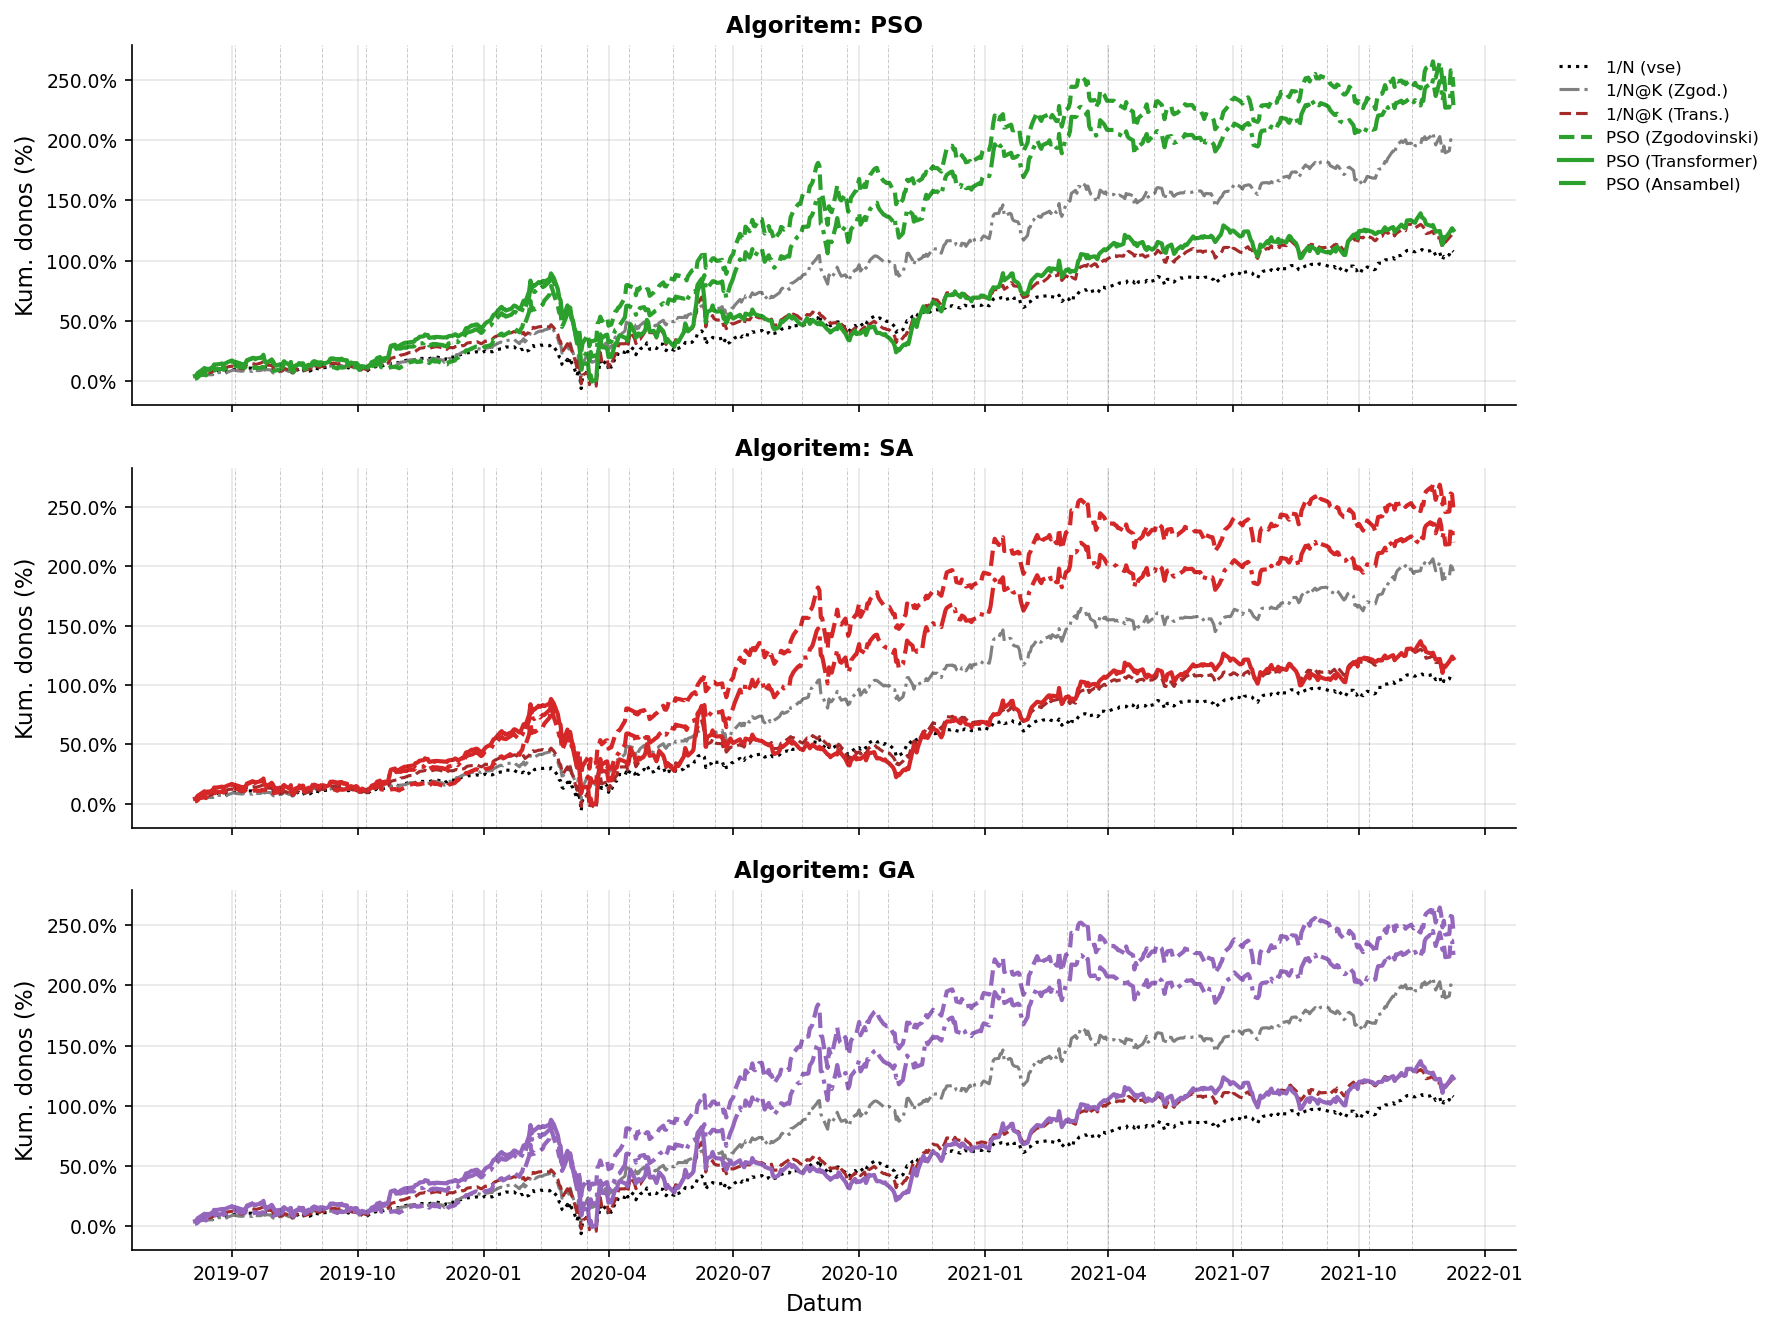
\includegraphics[height=0.30\textheight]{all_algorithms_grid_201906_202112_covid2020}\\[3pt]
  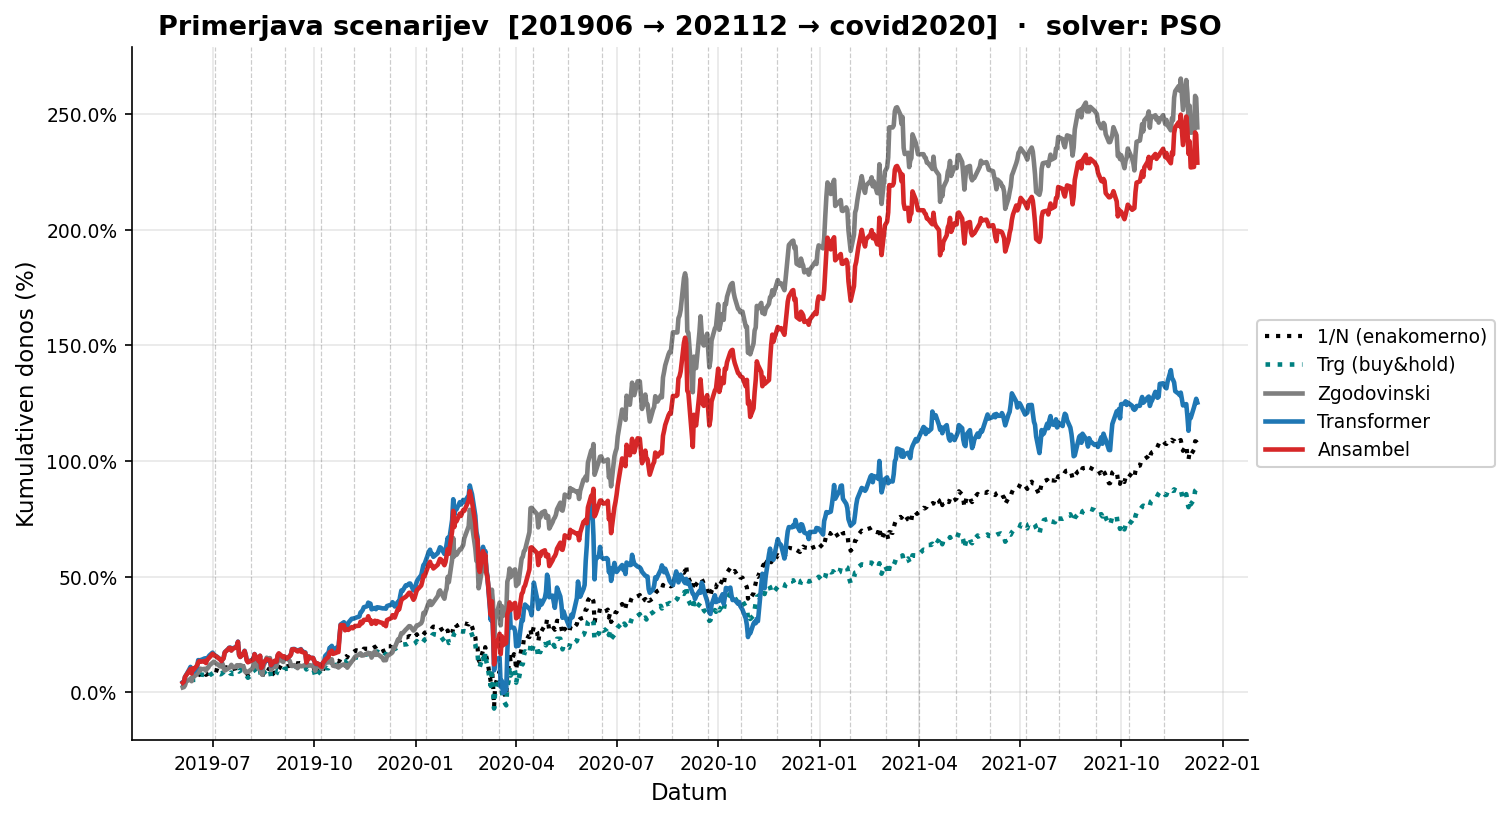
\includegraphics[height=0.30\textheight]{combined_walkforward_201906_202112_covid2020}\\[3pt]
  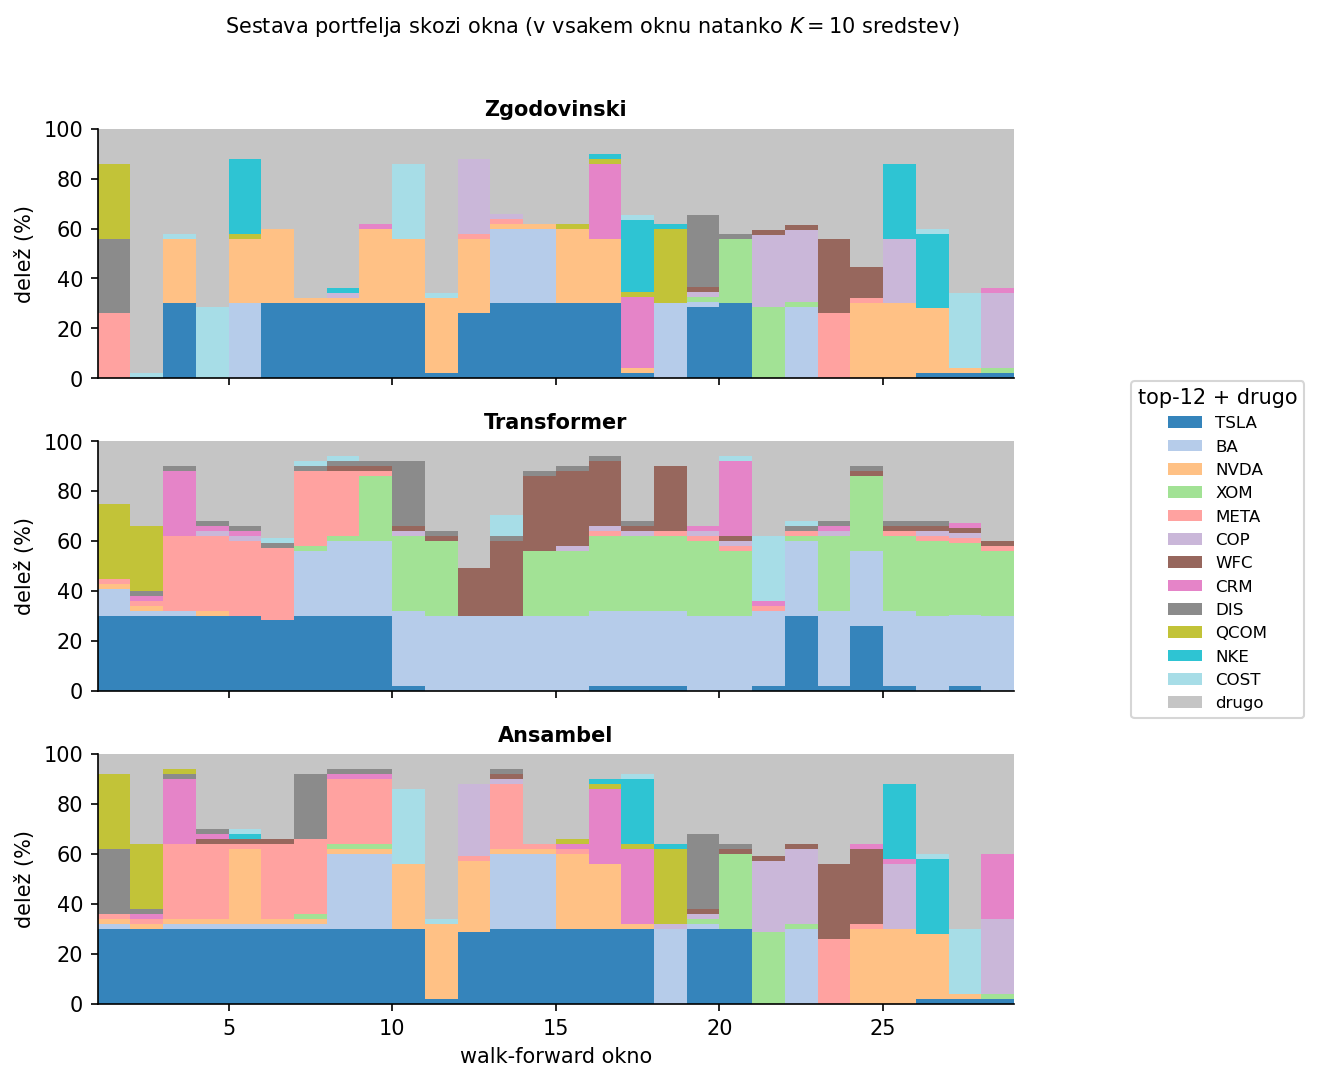
\includegraphics[height=0.26\textheight]{weights_top_201906_202112_covid2020}
  \caption{Režim pandemije COVID 2019--2021: (zgoraj) trije scenariji po metahevristikah; (sredina) zbirni prikaz z referencami --- edini režim, kjer zgodovinski prekaša transformer; (spodaj) sestava portfelja skozi okna.}
  \label{fig:reg-covid}
\end{figure}

\subsection{Obdobje dvigovanja obrestnih mer 2022--2024}
\label{sec:reg-2022}

Leto 2022 je zaznamovalo agresivno dvigovanje obrestnih mer in medvedji trg, ki mu je 2023--2024 sledilo okrevanje, poganjano z ozko skupino tehnoloških delnic. Sektorska razpršenost donosov je bila velika, kar nagrajuje presečno razvrščanje: transformer doseže Sharpe~$1{,}04$ in~$+92\,\%$ proti zgodovinskim~$0{,}47$ in~$+29\,\%$ (Tabeli~\ref{tab:regimes},~\ref{tab:regimescum}). Ansambel je tu med najboljšimi ($+100\,\%$) in celo prekaša oba posamezna eksperta, kar je skladno z mejo regreta Hedge. Slika~\ref{fig:reg-2022} kaže obvladan padec 2022 in sodelovanje v okrevanju 2023--2024 pri napovednih scenarijih.

\begin{figure}[p]
  \centering
  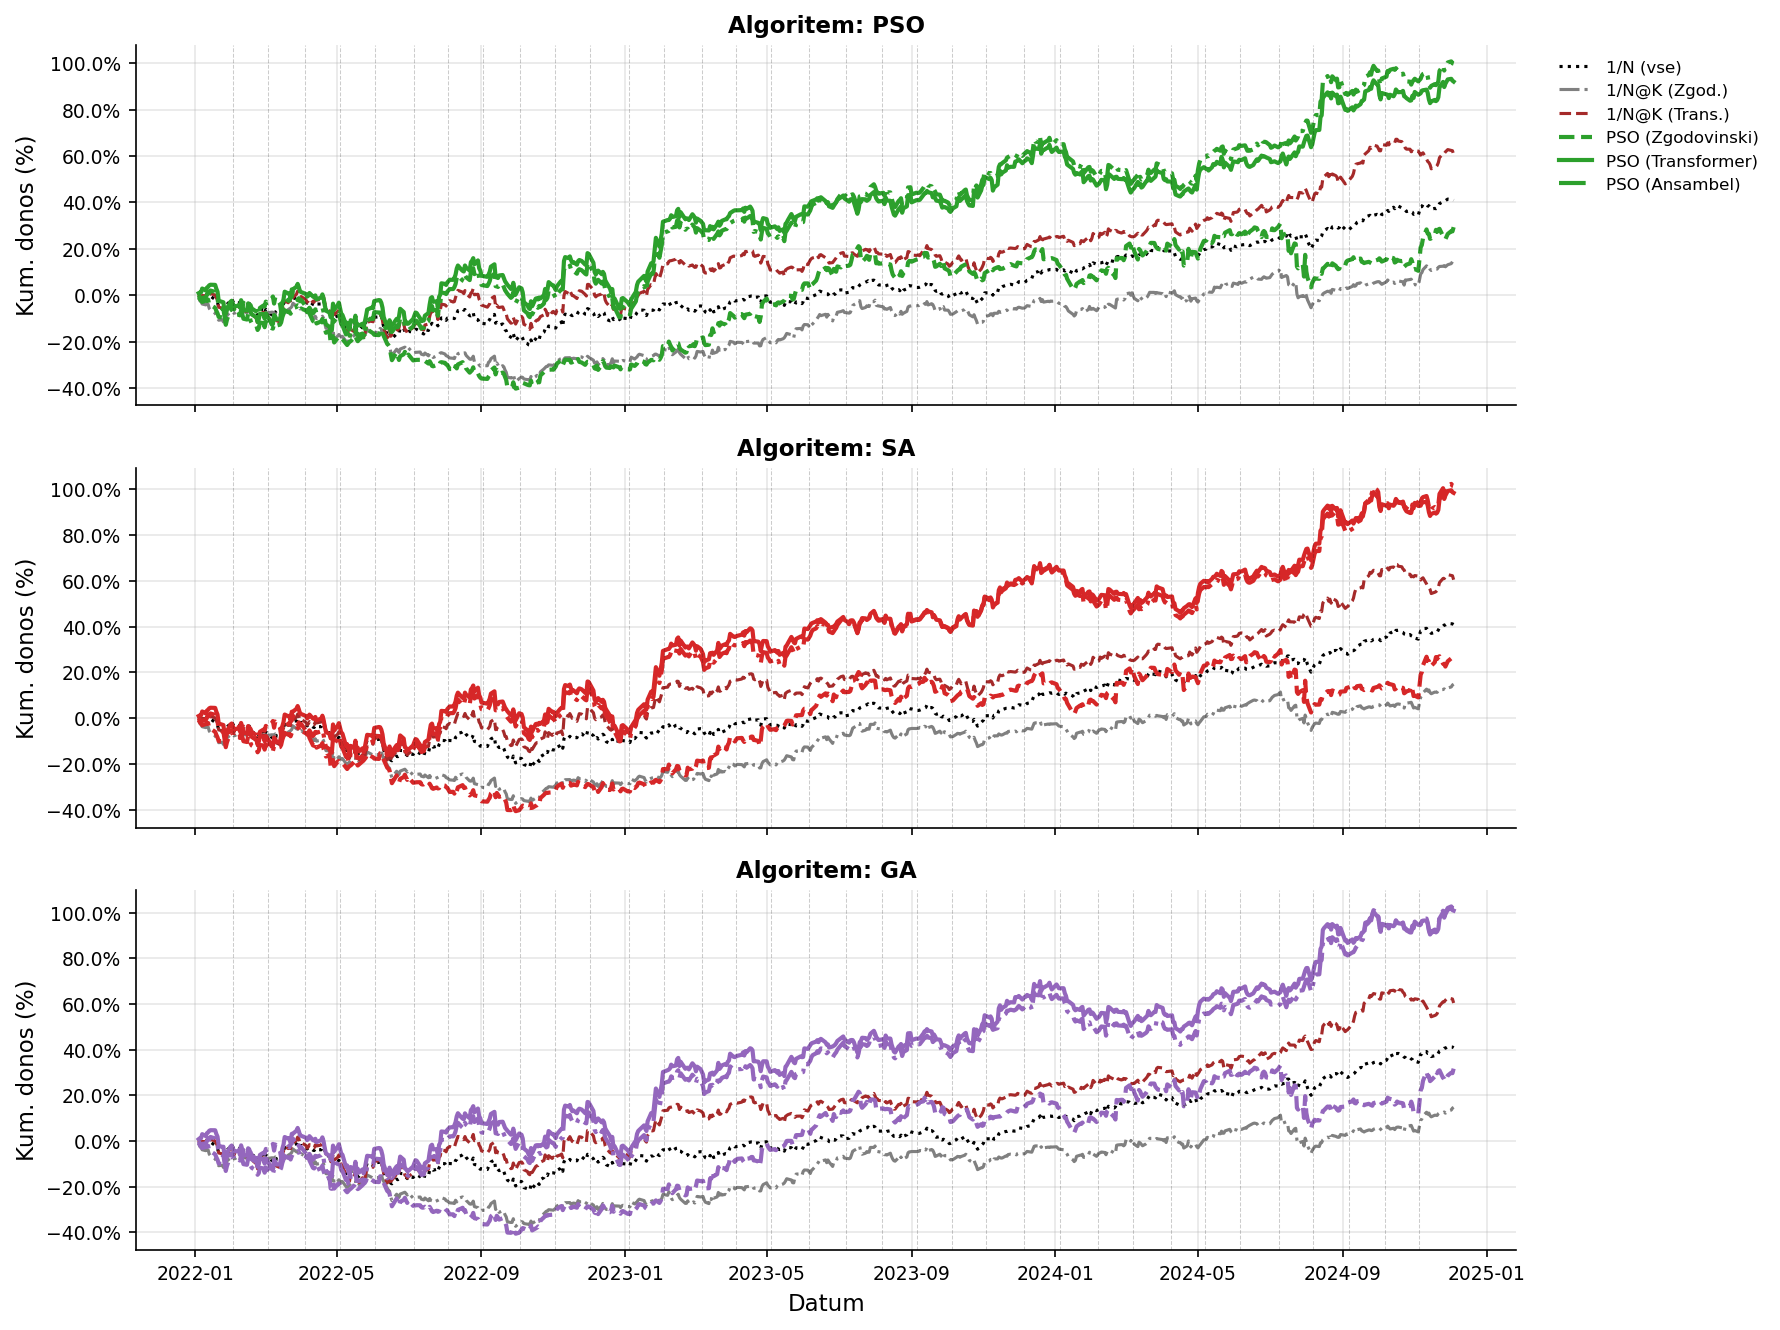
\includegraphics[height=0.30\textheight]{all_algorithms_grid_202201_202412}\\[3pt]
  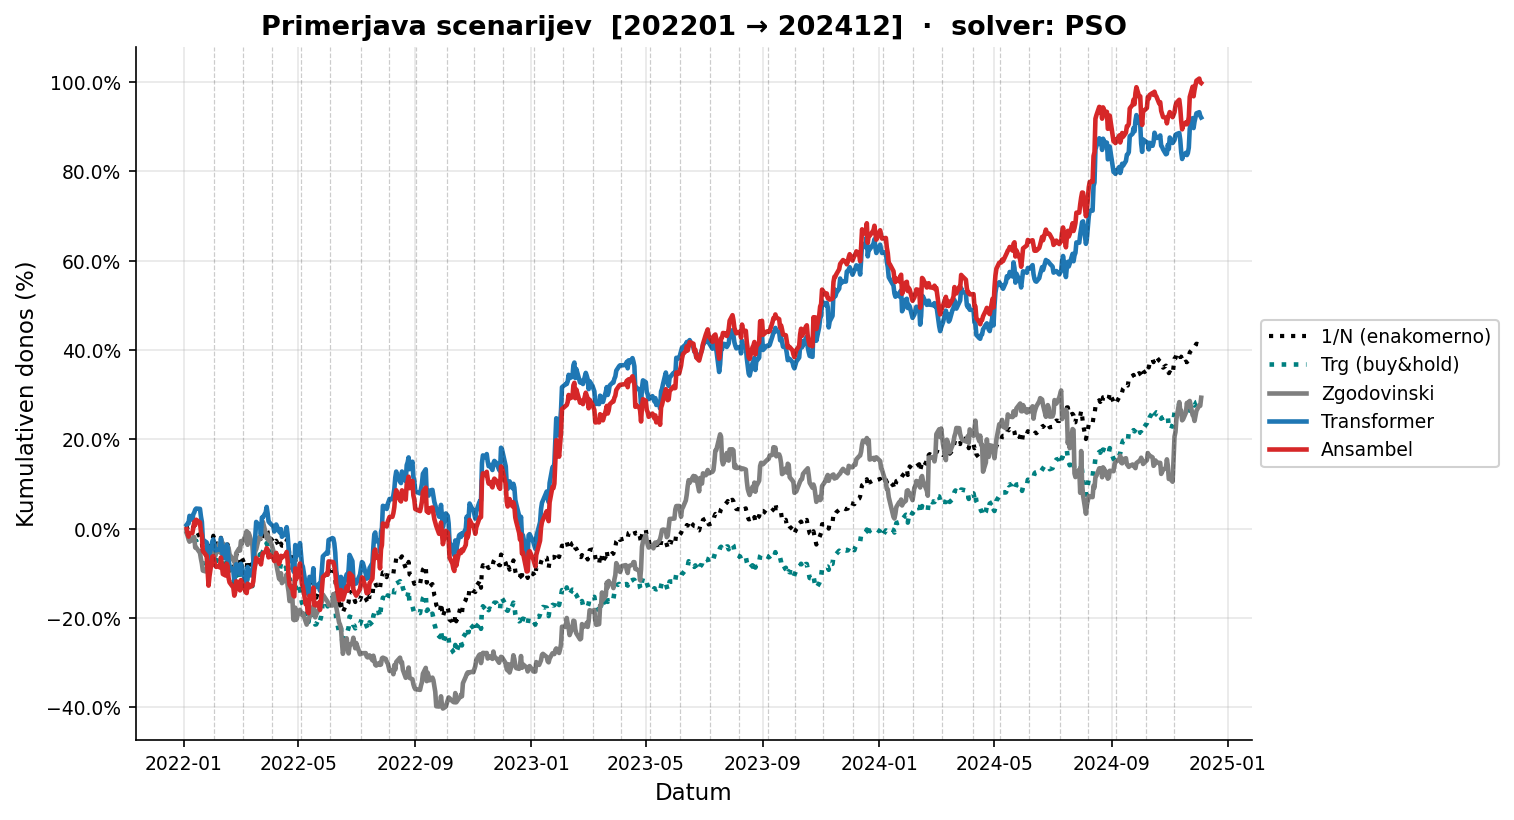
\includegraphics[height=0.30\textheight]{combined_walkforward_202201_202412}\\[3pt]
  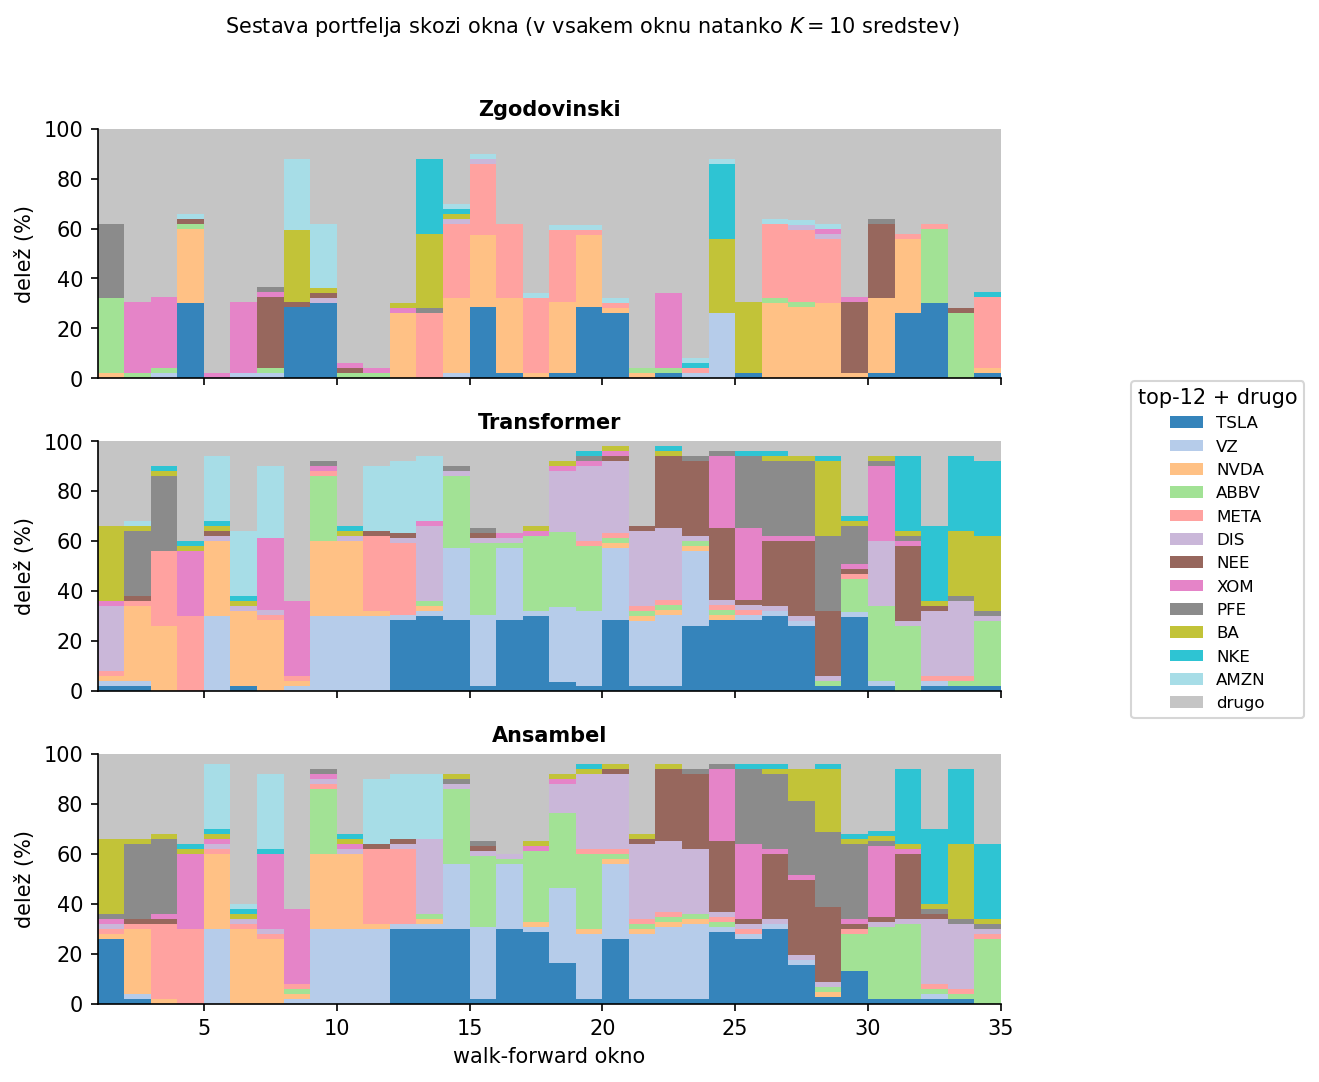
\includegraphics[height=0.26\textheight]{weights_top_202201_202412}
  \caption{Režim dvigovanja obrestnih mer 2022--2024: (zgoraj) trije scenariji po metahevristikah; (sredina) zbirni prikaz z referencami; (spodaj) sestava portfelja skozi okna.}
  \label{fig:reg-2022}
\end{figure}

\subsection{2019--2022 brez tehnoloških velikanov (divuniverse)}
\label{sec:reg-divuniverse}

Ta režim je namenjen naslavljanju pomisleka, da prednost transformerja izvira zgolj iz statične stave na peščico tehnoloških velikanov (Apple, Microsoft, Nvidia ipd.). Iz univerzuma jih zato izločimo. Rezultat je poučen: prednost transformerja se \emph{poveča}, ne zmanjša --- Sharpe~$1{,}27$ proti zgodovinskim~$0{,}28$ in~$+197\,\%$ proti~$+16\,\%$ (Tabeli~\ref{tab:regimes},~\ref{tab:regimescum}). To potrjuje, da model zajema splošen presečni signal, ne le trenda mega-kapitalizacij. Slika~\ref{fig:reg-divuniverse} (in zgornji panel Slike~\ref{fig:walkforward}) prikazuje jasen in vztrajen razhod med napovednim in zgodovinskim scenarijem že brez velikanov.

\begin{figure}[p]
  \centering
  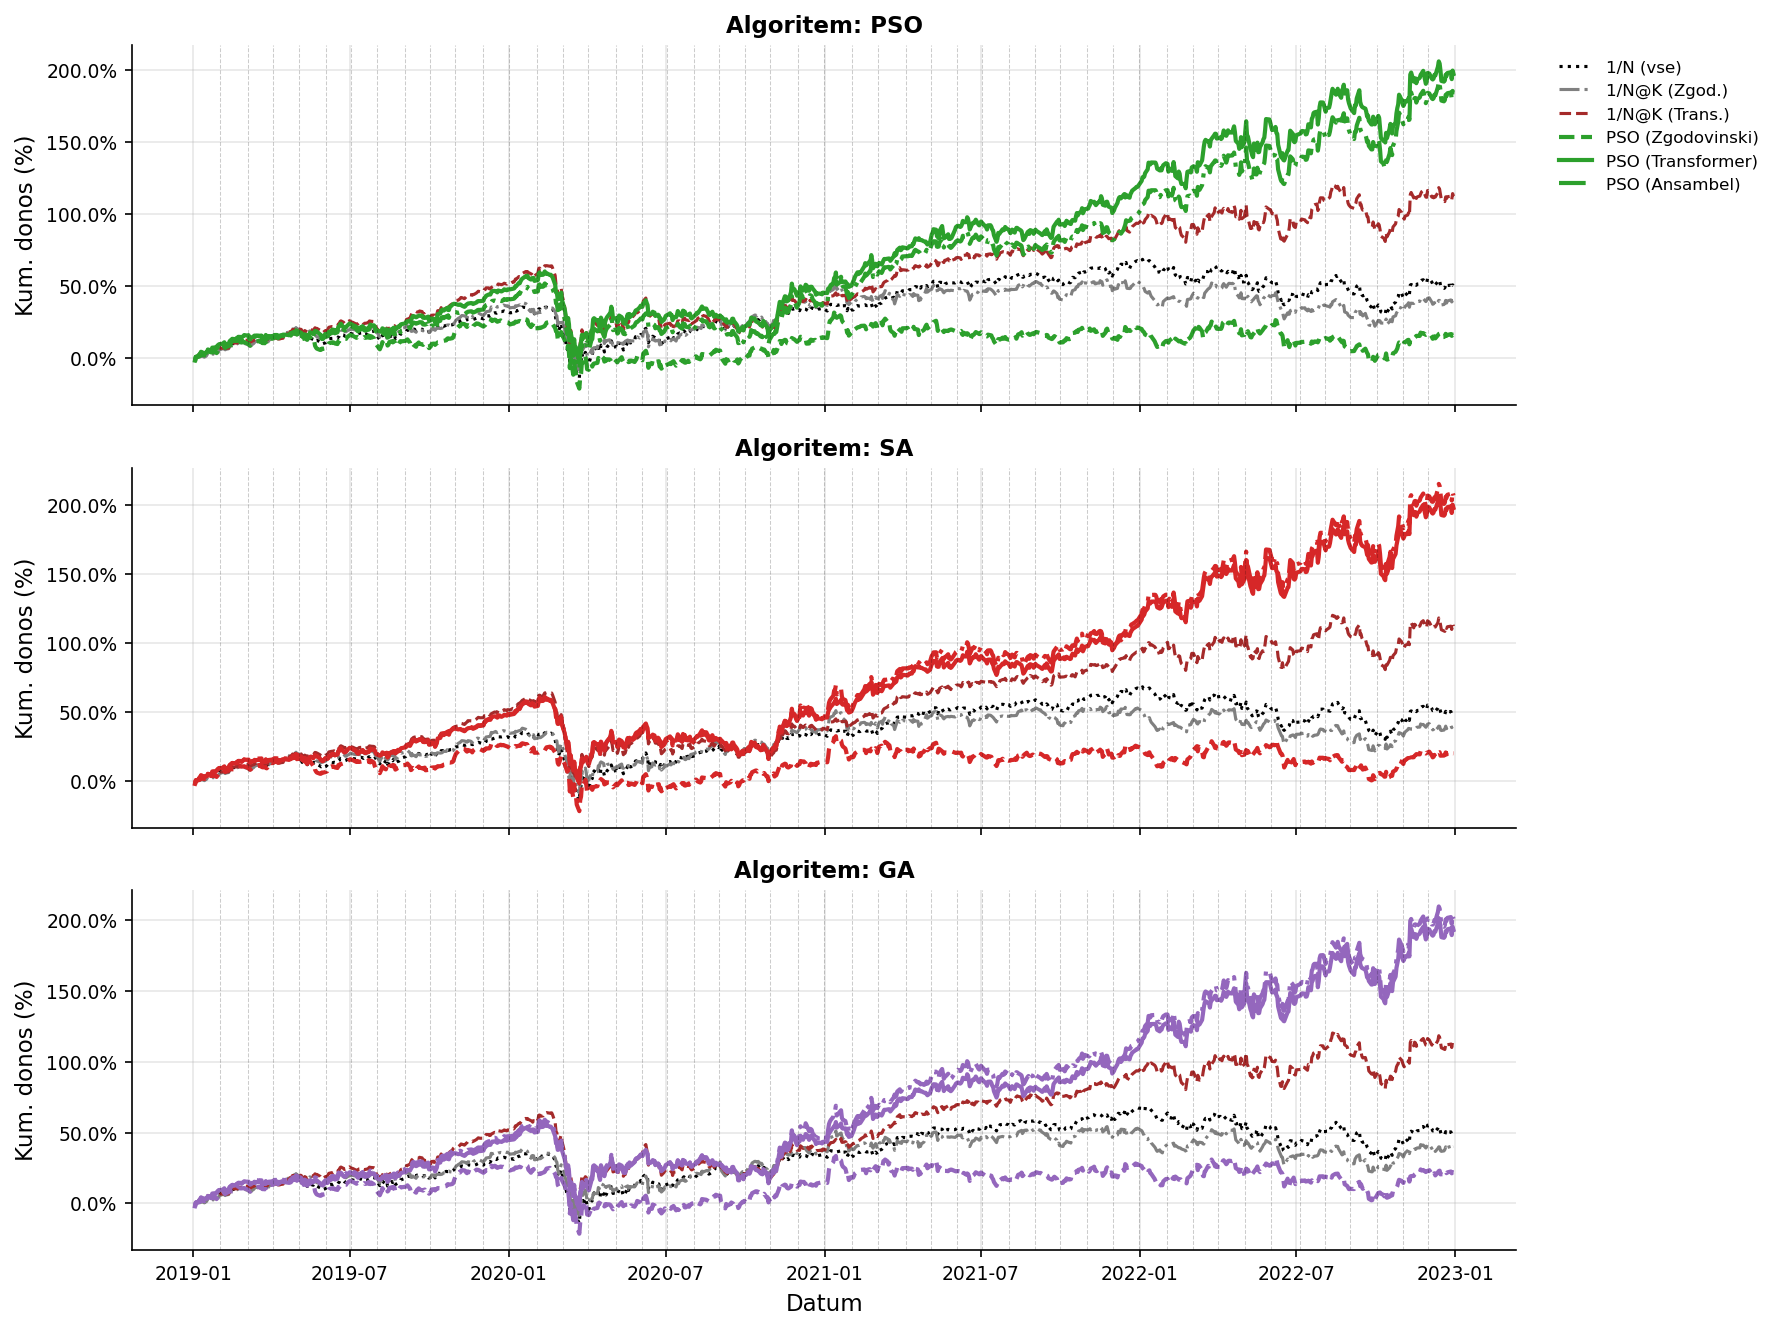
\includegraphics[height=0.30\textheight]{all_algorithms_grid_201901_202212_divuniverse}\\[3pt]
  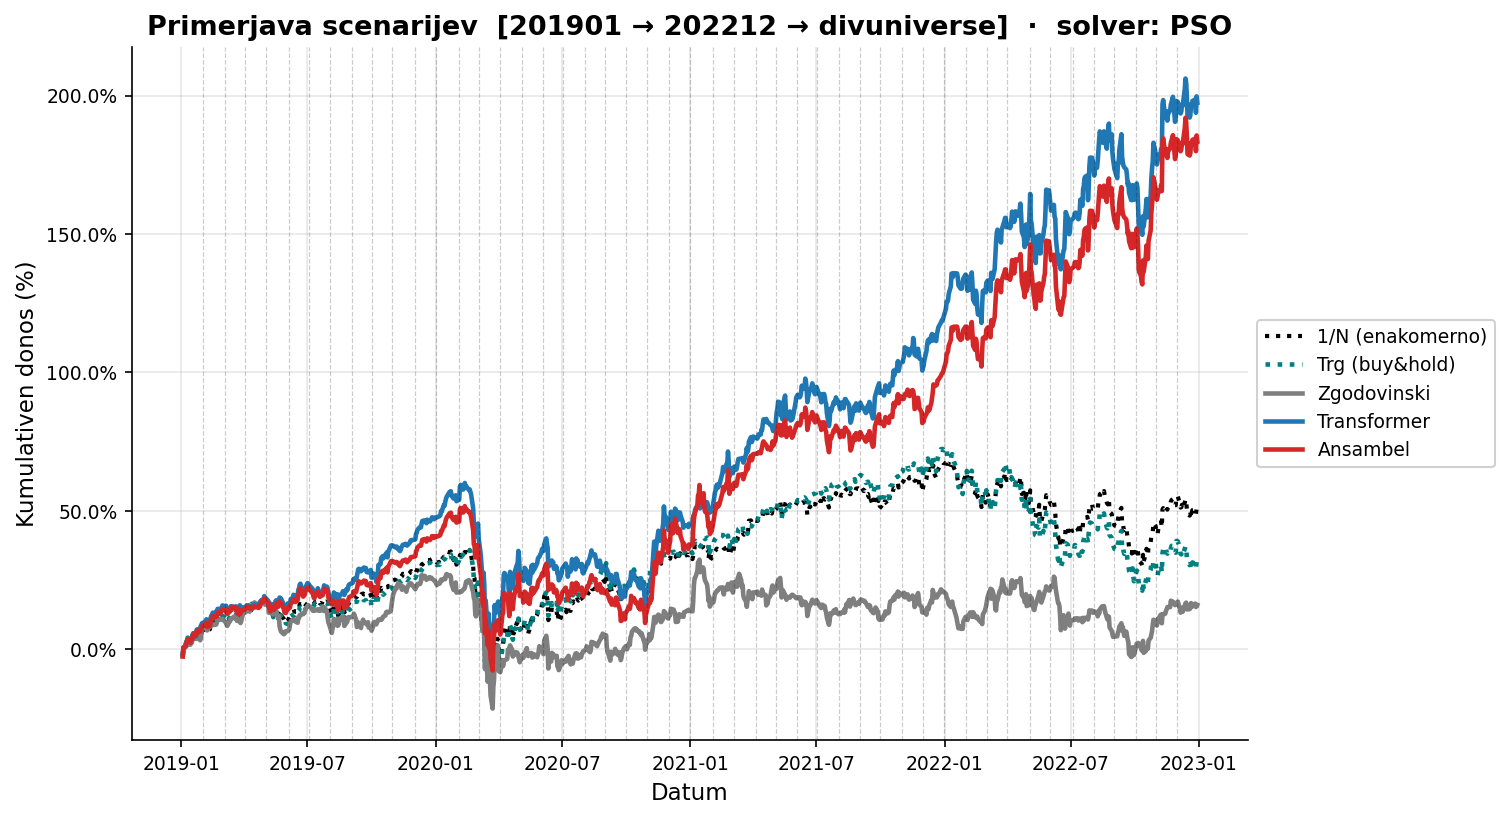
\includegraphics[height=0.30\textheight]{combined_walkforward_201901_202212_divuniverse}\\[3pt]
  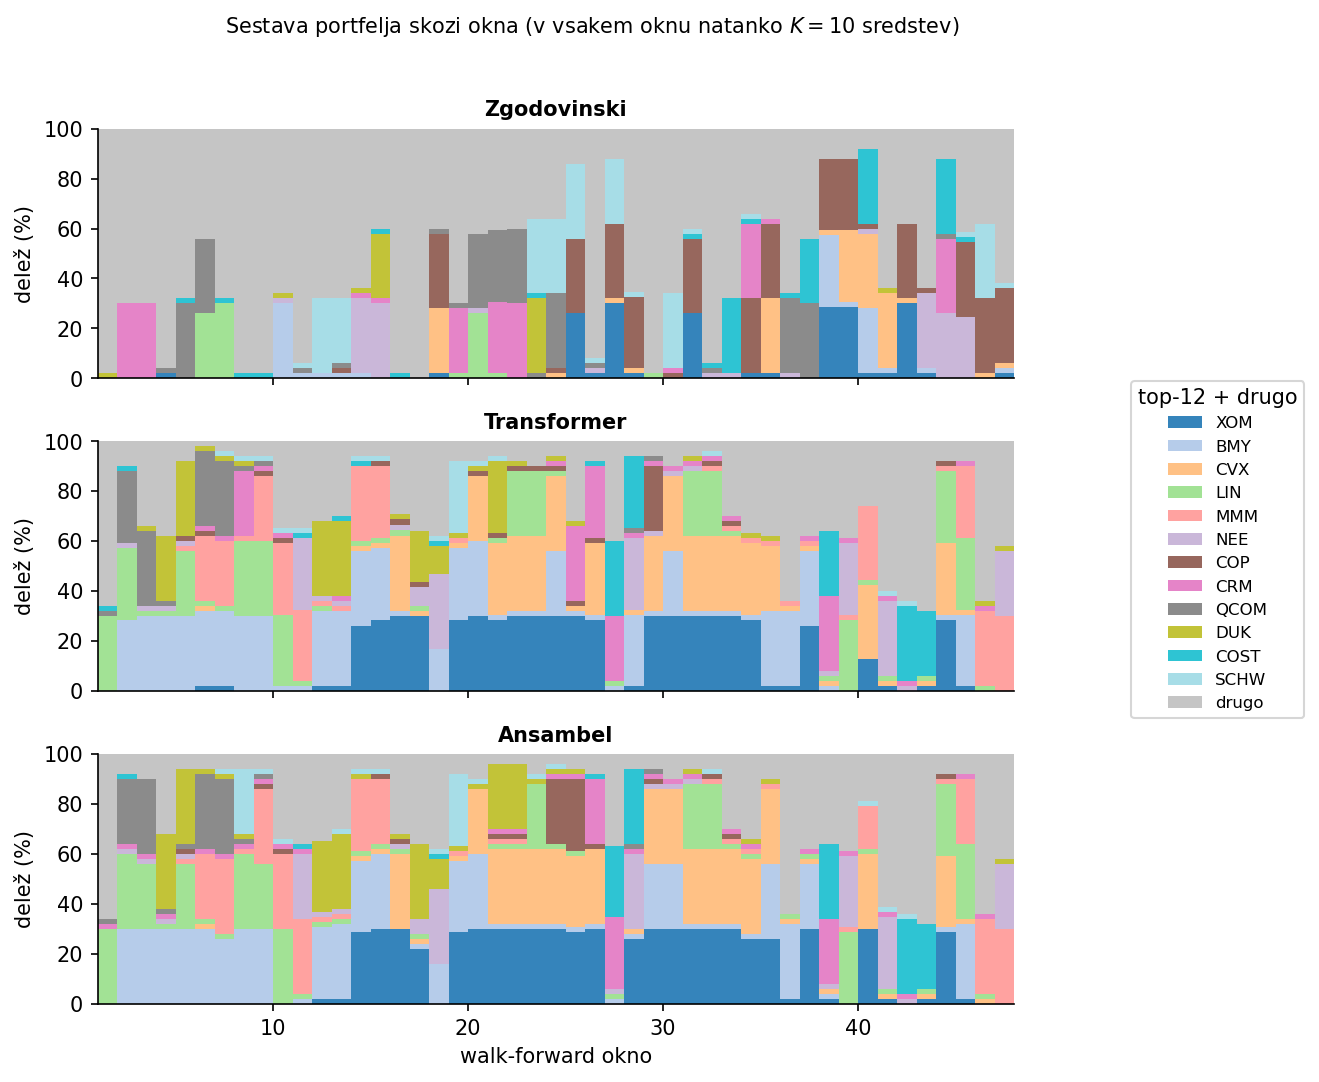
\includegraphics[height=0.26\textheight]{weights_top_201901_202212_divuniverse}
  \caption{Režim 2019--2022 brez tehnoloških velikanov (divuniverse): (zgoraj) trije scenariji po metahevristikah; (sredina) zbirni prikaz z referencami; (spodaj) sestava portfelja skozi okna --- brez mega-kapitalizacij.}
  \label{fig:reg-divuniverse}
\end{figure}

\subsection{2019--2022 s tehnološkimi velikani (headline)}
\label{sec:reg-headline}

V polnem univerzumu z vključenimi tehnološkimi velikani je obdobje 2019--2022 najtežje za razlikovanje med scenariji: nekaj velikank je poganjalo tako velik del donosa, da že naivni~$1/N$ doseže spodoben rezultat ($+60\,\%$, celo nad transformerjevim~$+42\,\%$ v končnem donosu; Tabela~\ref{tab:regimescum}). Transformer in zgodovinski scenarij dosežeta enak Sharpe ($0{,}43$; Tabela~\ref{tab:regimes}), LSTM pa je tu izjemoma nekoliko boljši ($0{,}62$). To je pošten primer režima, kjer koncentrirana zmagovalna sredstva zabrišejo prednost presečnega razvrščanja. Slika~\ref{fig:reg-headline} kaže tesno prepletene scenarije; prav kontrast s prejšnjim (divuniverse) razkrije, da so velikani tu ``dvignili vse čolne''.

\begin{figure}[p]
  \centering
  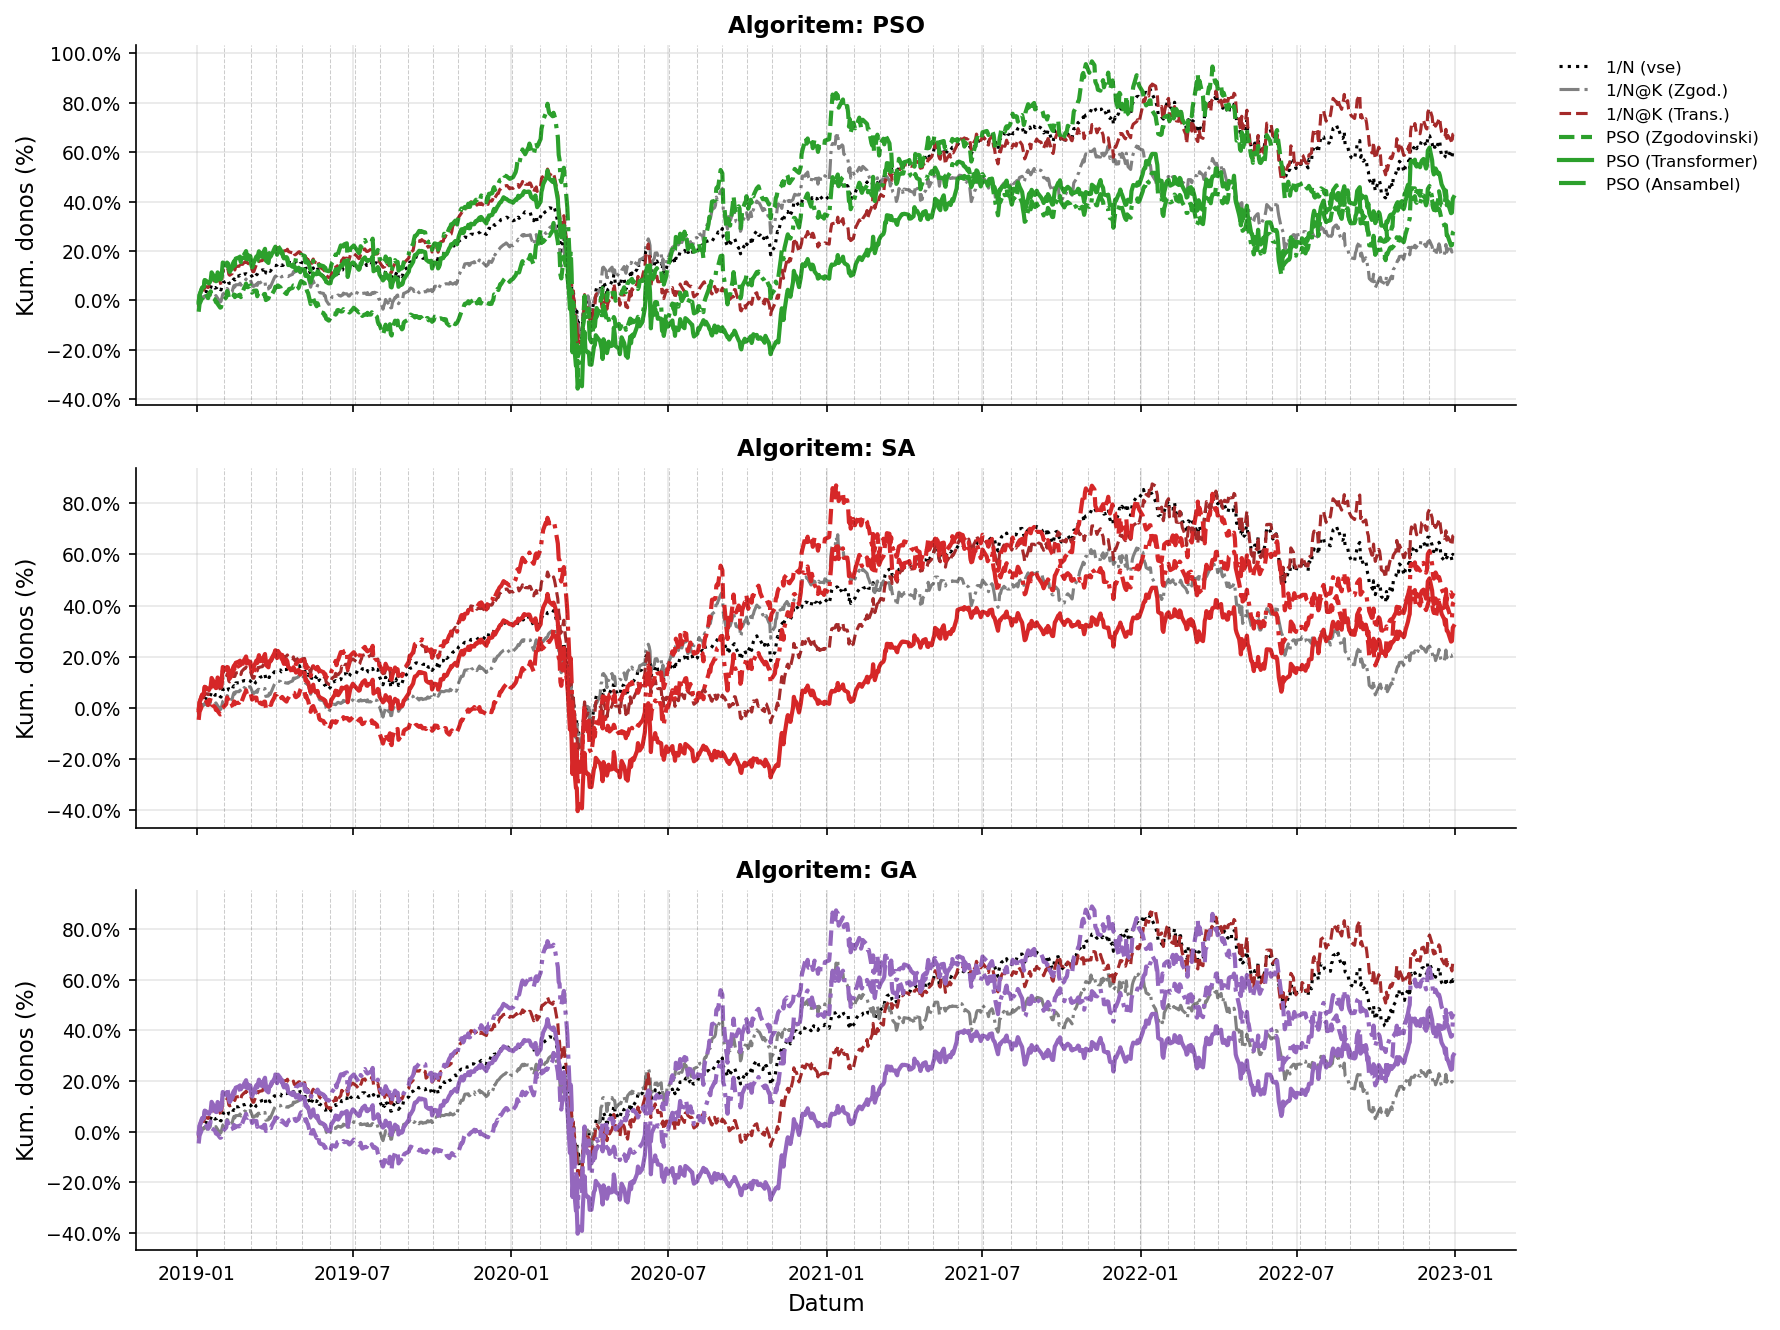
\includegraphics[height=0.30\textheight]{all_algorithms_grid_201901_202212}\\[3pt]
  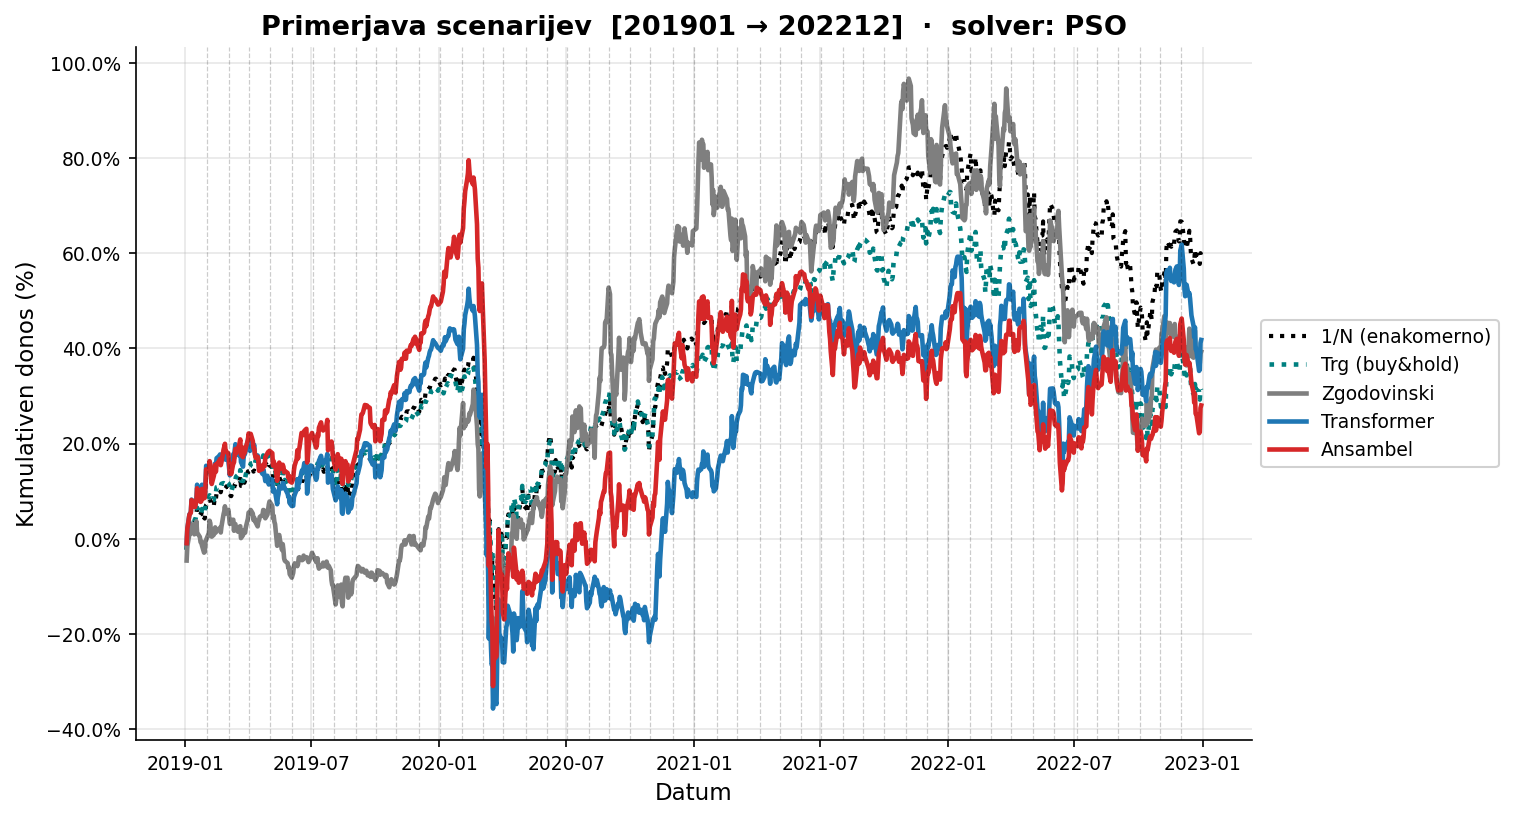
\includegraphics[height=0.30\textheight]{combined_walkforward_201901_202212}\\[3pt]
  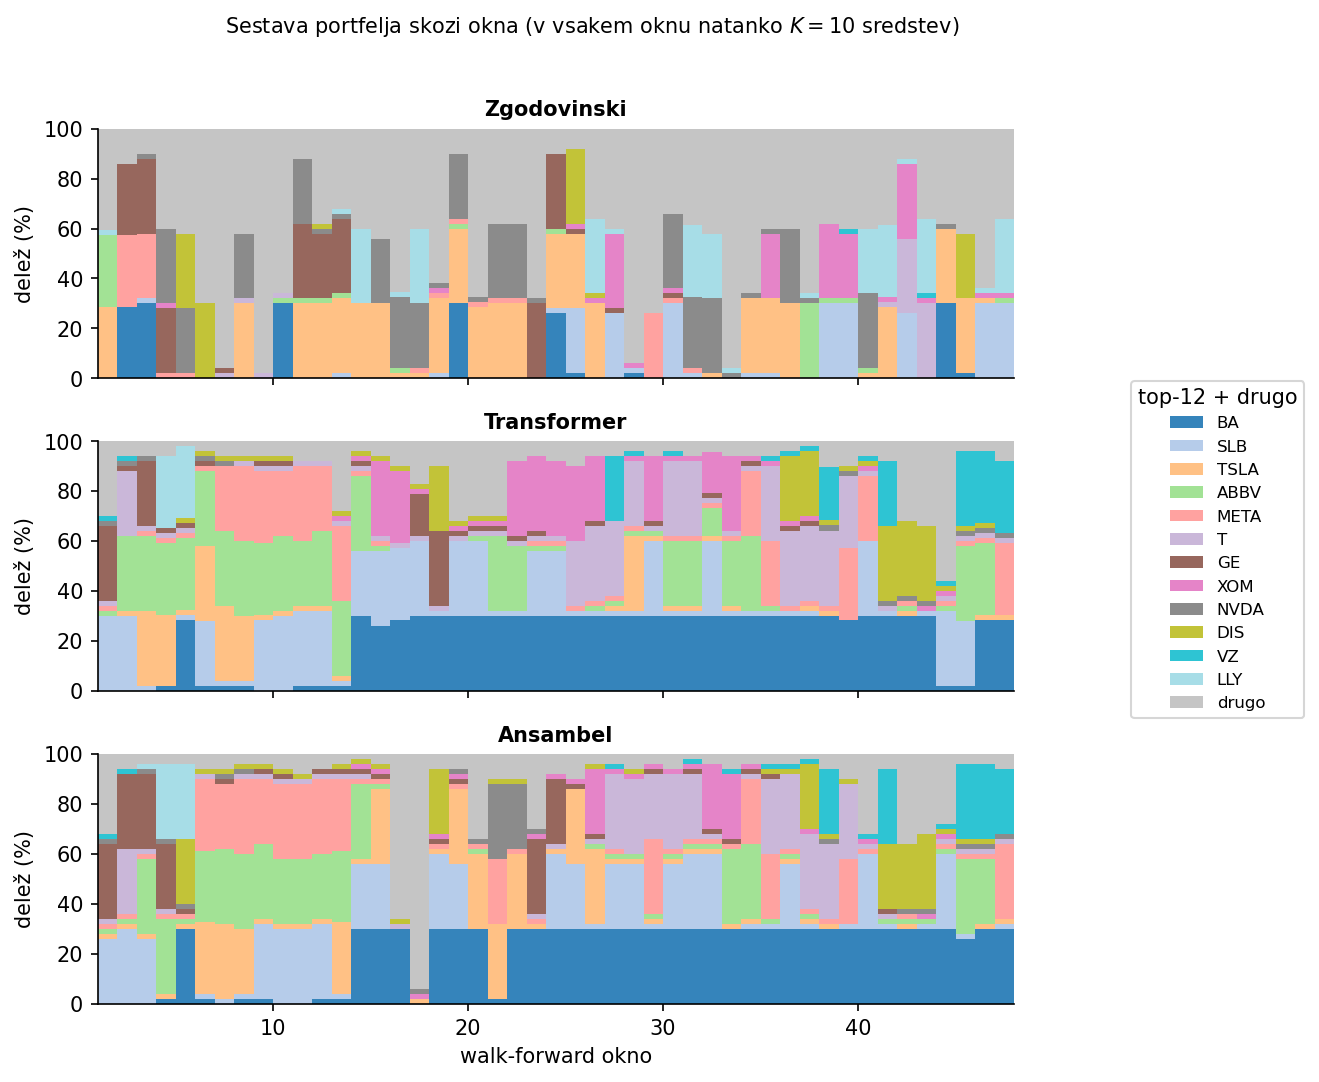
\includegraphics[height=0.26\textheight]{weights_top_201901_202212}
  \caption{Režim 2019--2022 s tehnološkimi velikani (headline): (zgoraj) trije scenariji po metahevristikah; (sredina) zbirni prikaz z referencami; (spodaj) sestava portfelja skozi okna --- s koncentracijo v mega-kapitalizacije.}
  \label{fig:reg-headline}
\end{figure}

\subsection{Neposredna primerjava: protokol Ramos in sod.\ (S\&P 100, 2011--2021)}
\label{sec:reg-ramos}

Za zunanjo veljavnost cevovod poženemo na protokolu Ramos in sod.~\cite{ramos2023} (S\&P~100, 2011--2021, kardinalna omejitev do~$20$ sredstev, drseče okno,~$30$~bazičnih točk). Gre za dolgo, pretežno bikovsko desetletje z vmesnimi popravki (2011, 2015--2016, 2018). Naš transformerski cevovod doseže letni Sharpe~$1{,}11$ (ansambel~$1{,}07$), kar preseže njihovo objavljeno referenco indeksa S\&P~100 ($0{,}99$; razdelek~\ref{sec:headtohead}). Slika~\ref{fig:reg-ramos} prikazuje potek na tem protokolu; ker se ciljna funkcija in omejitve ne ujemajo povsem z izvirno študijo, je primerjava na ravni metrike.

\begin{figure}[p]
  \centering
  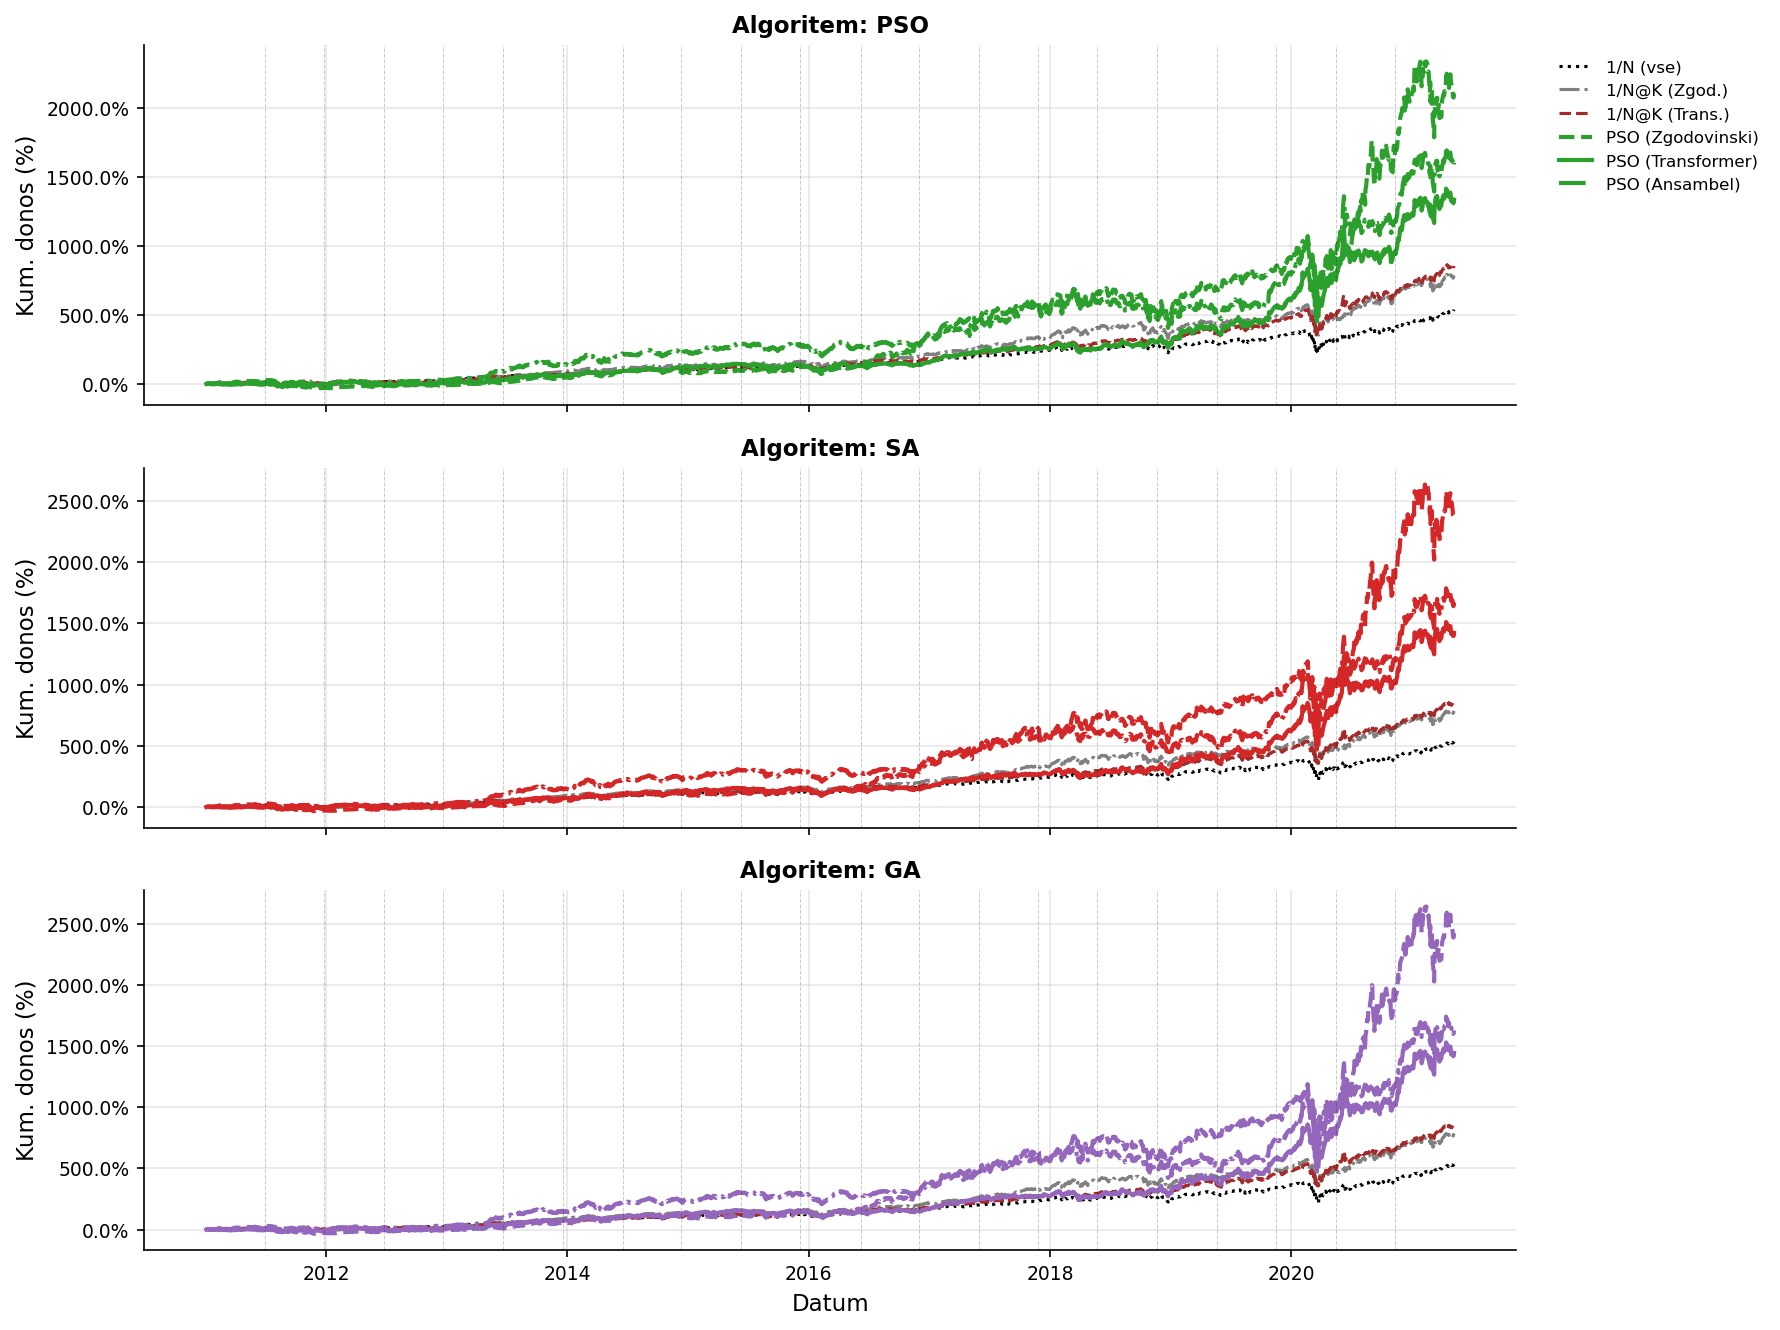
\includegraphics[height=0.30\textheight]{all_algorithms_grid_201101_202106}\\[3pt]
  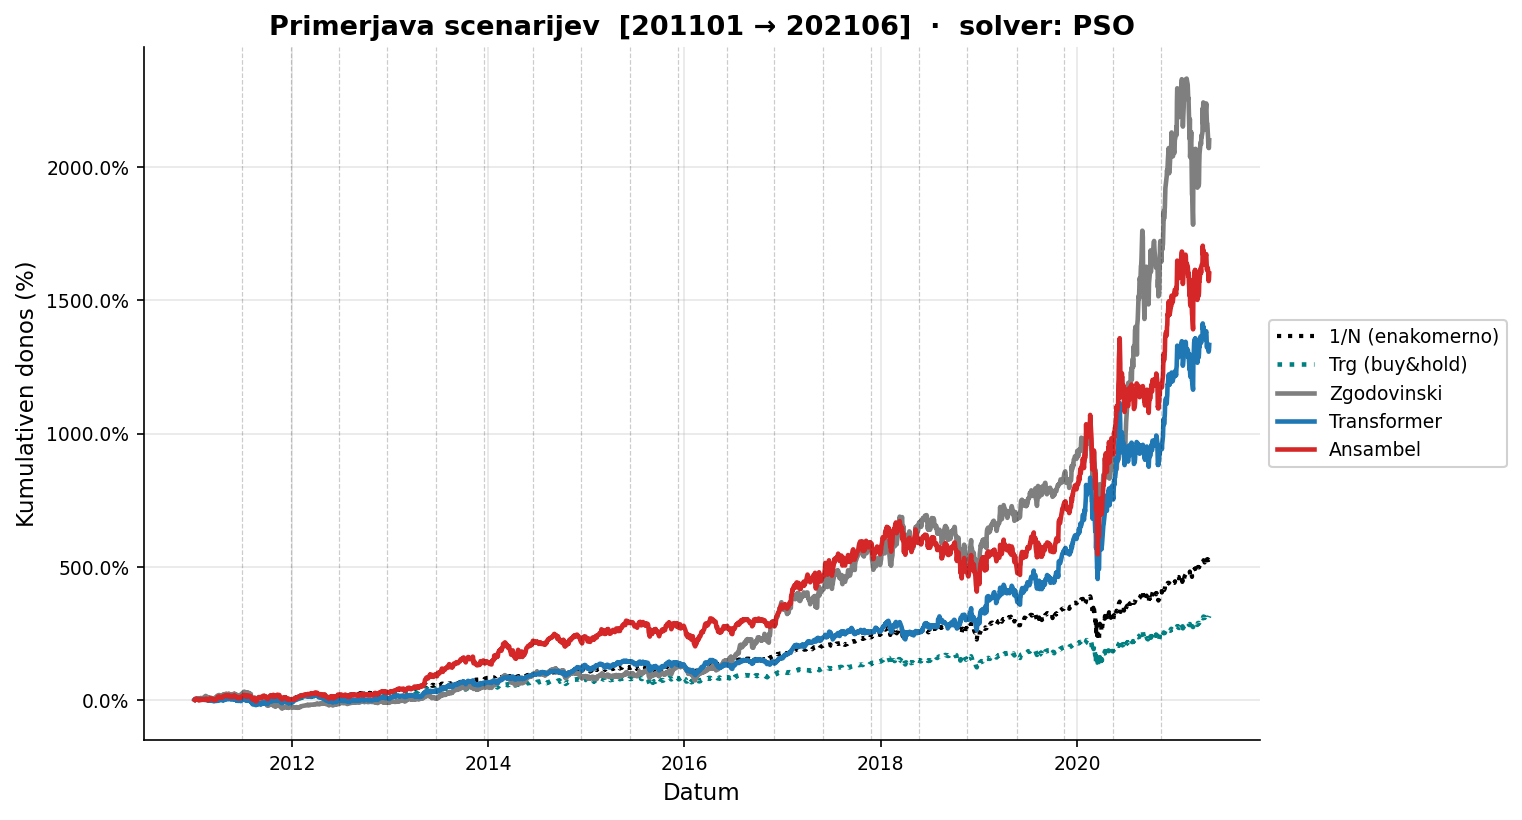
\includegraphics[height=0.30\textheight]{combined_walkforward_201101_202106}\\[3pt]
  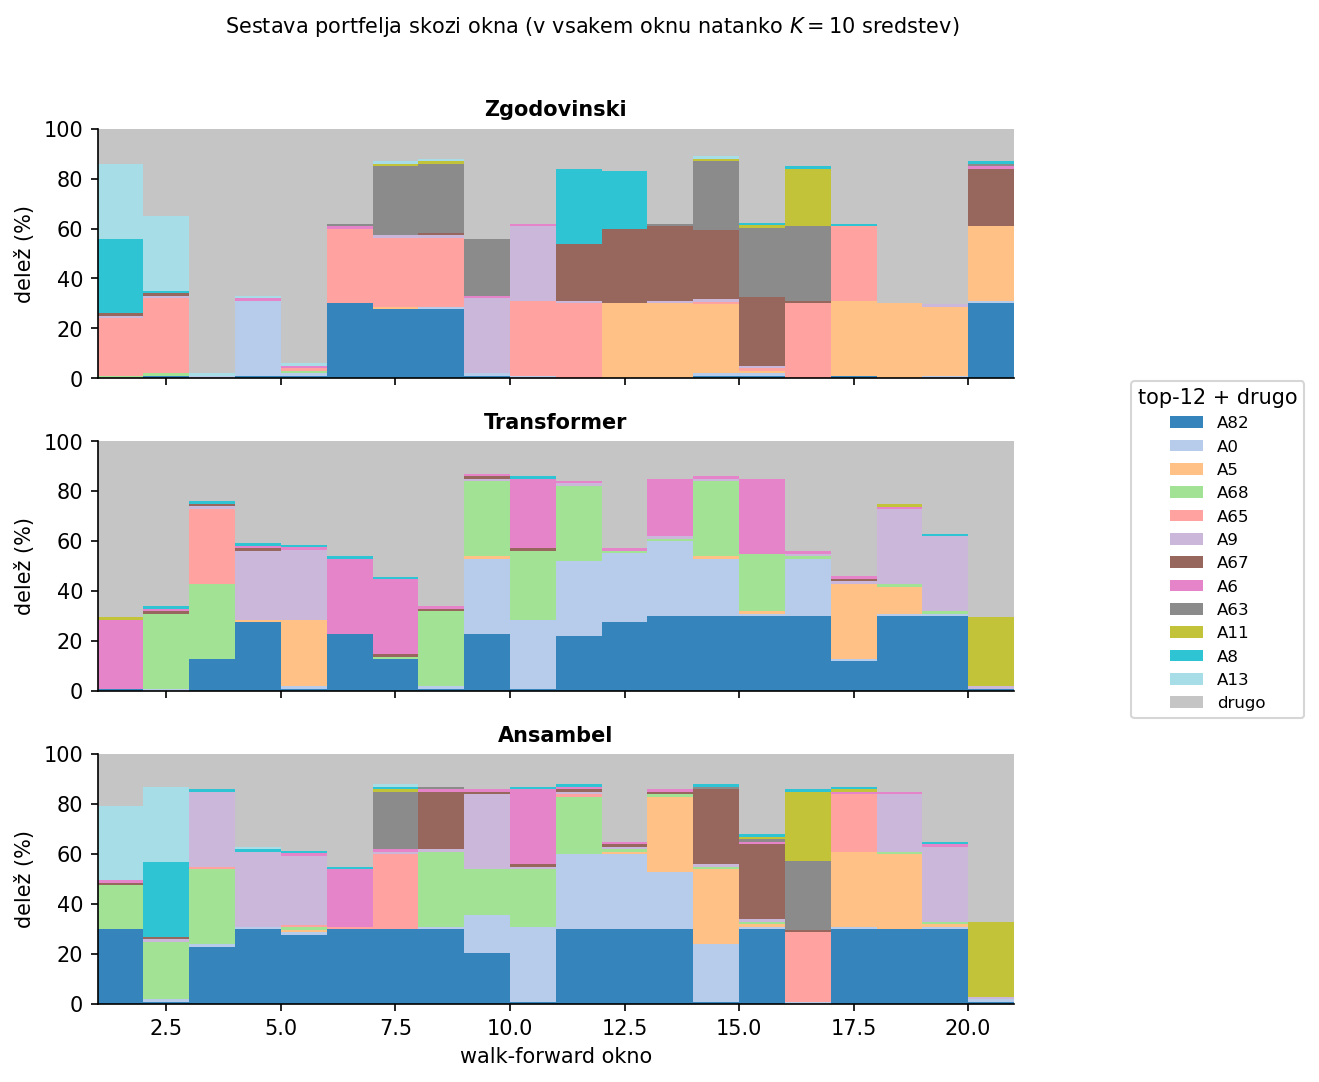
\includegraphics[height=0.26\textheight]{weights_top_201101_202106}
  \caption{Neposredna primerjava na protokolu Ramos in sod.\ (S\&P~100, 2011--2021): (zgoraj) trije scenariji po metahevristikah; (sredina) zbirni prikaz z referencami; (spodaj) sestava portfelja skozi okna.}
  \label{fig:reg-ramos}
\end{figure}

\subsection{Neposredna primerjava: protokol Fernandes in Desell (50 delnic S\&P 500, 2022--2023)}
\label{sec:reg-fernandes}

Drugi zunanji protokol je Fernandes in Desell~\cite{fernandes2026} ($50$~delnic S\&P~500, 2022--2023, četrtletno rebalansiranje, s stroški). To je kratko, volatilno obdobje (medvedji trg 2022, delno okrevanje 2023). Naš cevovod doseže Sharpe~$0{,}77$ proti njihovemu najboljšemu modelu (AttentionLSTM,~$0{,}29$), in to ob \emph{strožji} kardinalni omejitvi ($K{=}10$ namesto njihovih~$50$; razdelek~\ref{sec:headtohead}). Slika~\ref{fig:reg-fernandes} prikazuje potek; strožja kardinalnost pomeni bolj koncentriran portfelj, kar je pri tako kratkem horizontu razvidno iz večjega obrata v sestavi.

\begin{figure}[p]
  \centering
  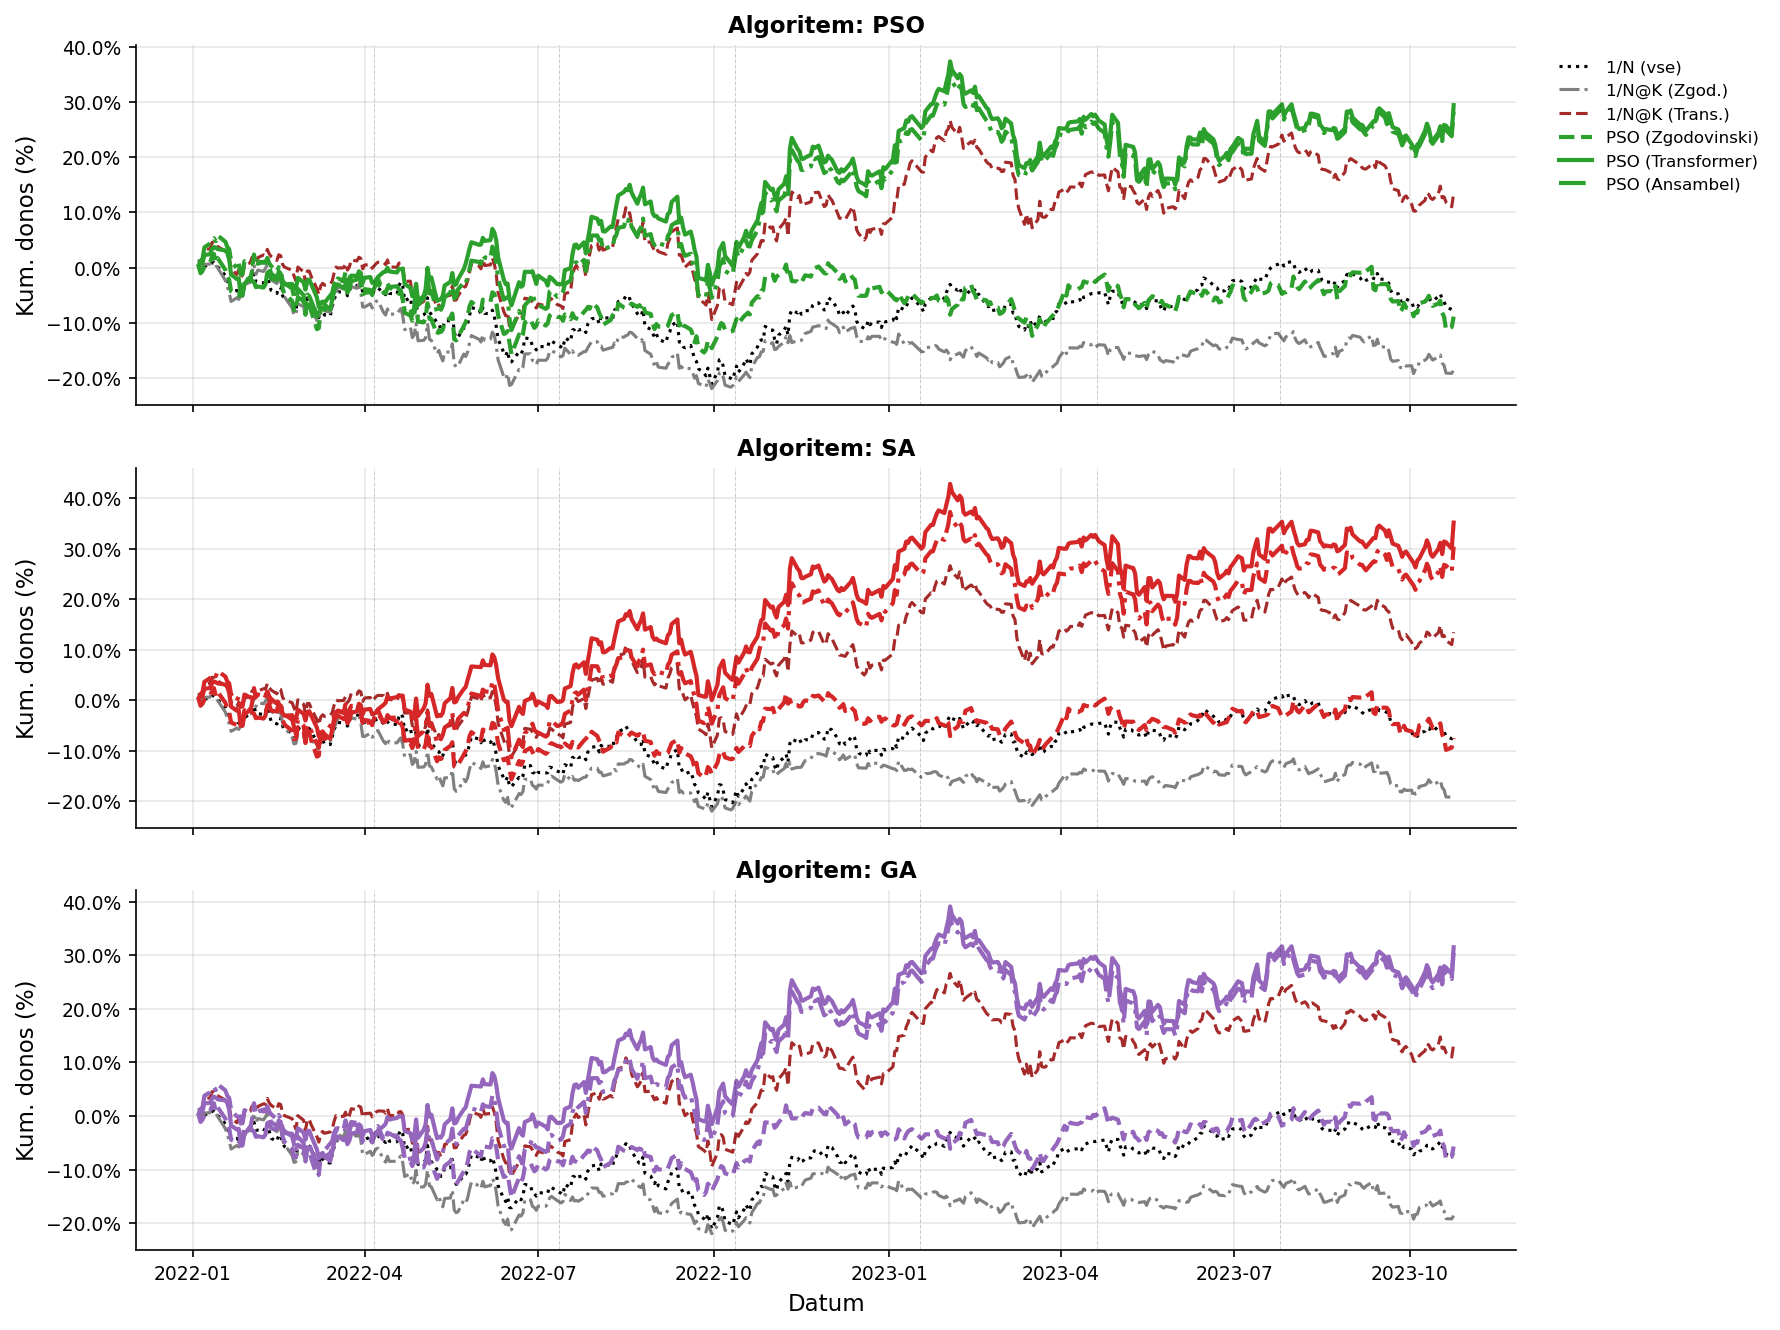
\includegraphics[height=0.30\textheight]{all_algorithms_grid_202201_202312}\\[3pt]
  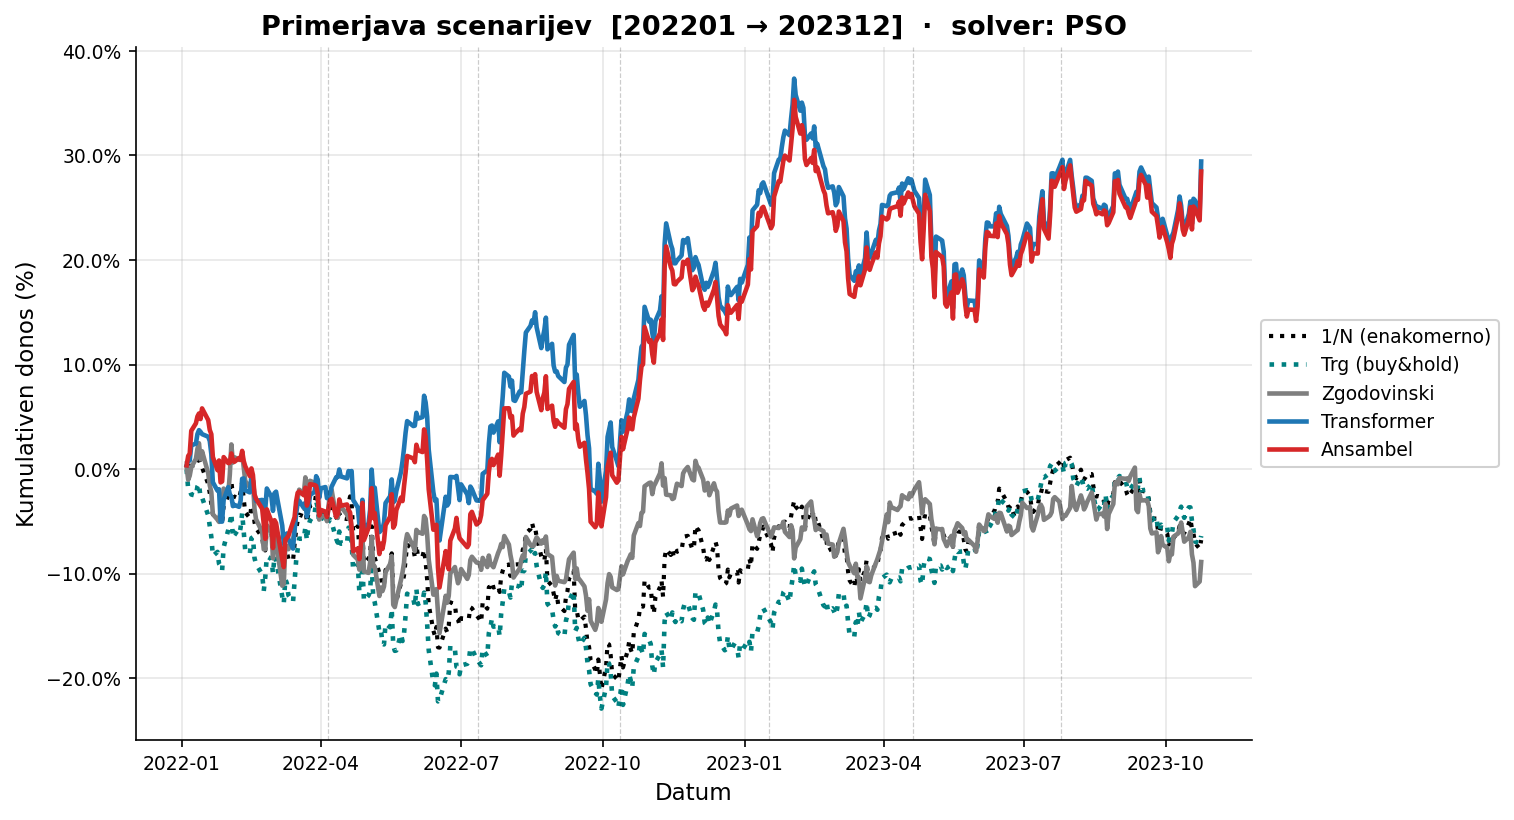
\includegraphics[height=0.30\textheight]{combined_walkforward_202201_202312}\\[3pt]
  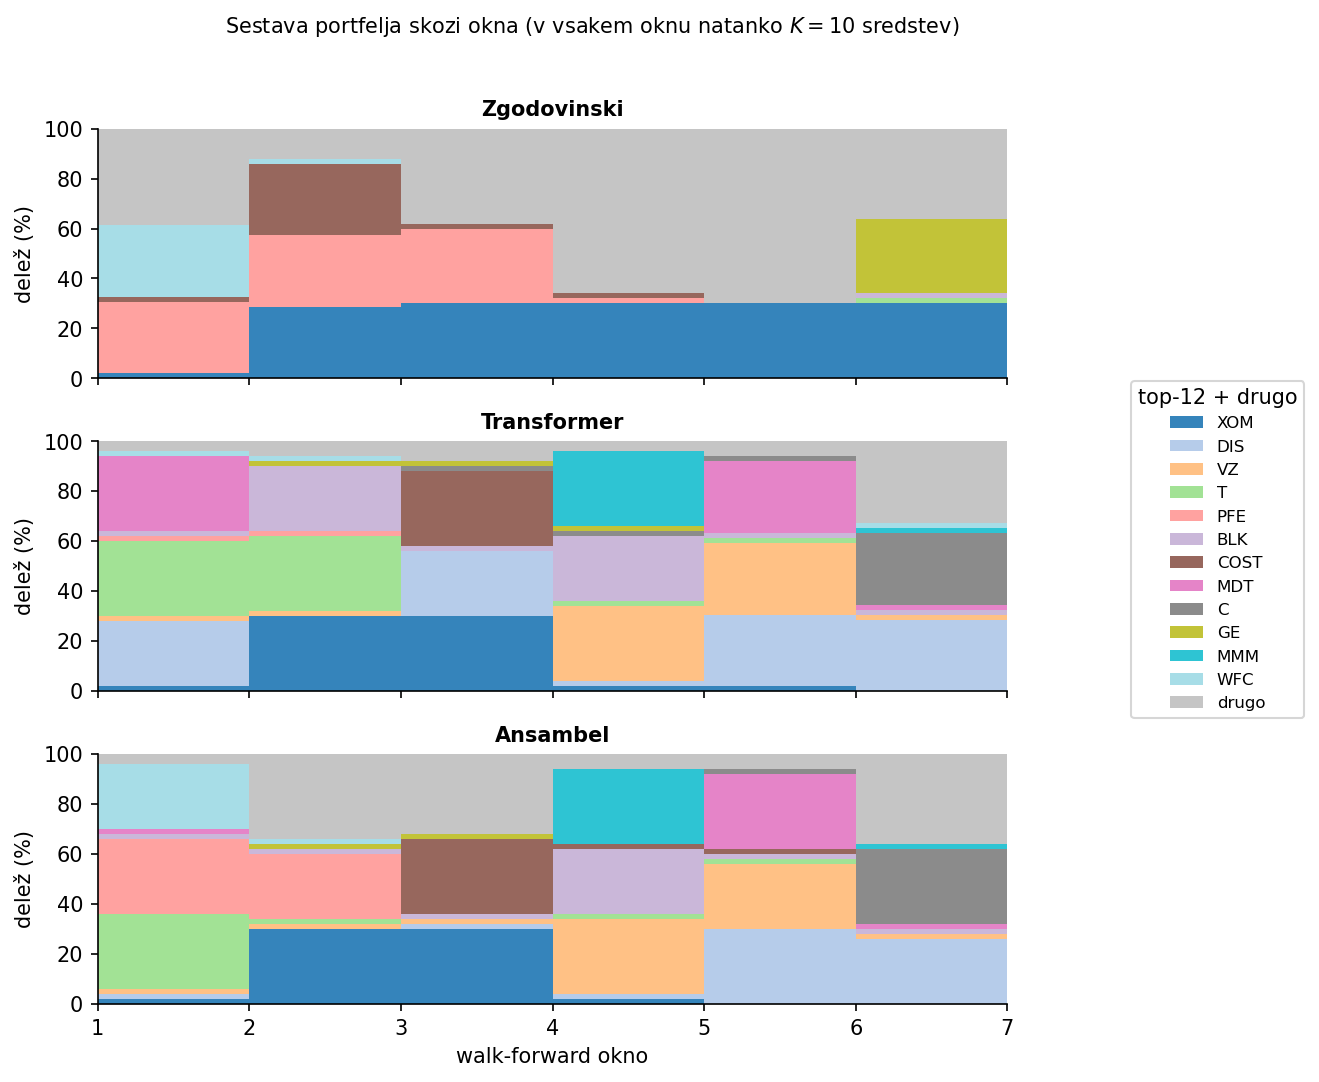
\includegraphics[height=0.26\textheight]{weights_top_202201_202312}
  \caption{Neposredna primerjava na protokolu Fernandes in Desell (50 delnic S\&P~500, 2022--2023): (zgoraj) trije scenariji po metahevristikah; (sredina) zbirni prikaz z referencami; (spodaj) sestava portfelja skozi okna.}
  \label{fig:reg-fernandes}
\end{figure}

\section{Pot do končne zasnove in ponovljivost}
\label{sec:pot}

Za pošteno oceno je pomembno dokumentirati tudi \emph{pot} do končne zasnove --- odločitve, ki so se izkazale za pravilne, in poskuse, ki niso pomagali.

\paragraph{Odkrita napaka pri razmejitvi podatkov.} V eni od zgodnjih konfiguracij (COVID) se je učno obdobje napovednega modela končalo \emph{po} začetku testa, kar je pomenilo, da je zamrznjeni model del zgodnjih testnih oken videl že med učenjem. Napako smo prepoznali in odpravili tako, da se učenje konča strogo pred prvim testnim oknom. Napaka je zadevala izključno ta režim; ostali so bili od začetka pravilno razmejeni.

\paragraph{Nevtralni razvrstitvenik namesto poudarjanja zmagovalcev.} Preučili smo možnost, da učno izgubo nagnemo k ``zmagovalcem'' (utež~$\alpha>0$). Takšen nagib res poveča donos v izrazito trendnih obdobjih (npr.\ vzpon peščice tehnoloških velikanov), a je \emph{režimsko toksičen}: v obdobjih vračanja k sredini poslabša napovedi. Ker je cilj \emph{robusten} model, smo se odločili za nevtralni razvrstitvenik ($\alpha=0$), ki v petih od šestih režimov premaga zgodovinsko referenco, poudarjanje zmagovalcev pa ohranili le kot možnost za analizo občutljivosti.

\paragraph{Poskusi robustifikacije, ki niso pomagali.} Da bi izboljšali edini režim, kjer transformer zaostane (okrevanje po pandemiji), smo preizkusili tri literaturno podprte pristope: (1)~\emph{periodično doučevanje} modela na rastoči zgodovini, (2)~\emph{distribucijsko robustno učenje} po najslabši skupini (Group DRO) glede na volatilnostne režime in (3)~\emph{winsorizacijo} normiranih vhodov proti režimskemu premiku. Vsi trije so v tem režimu bodisi poslabšali bodisi niso opazno spremenili rezultata; pri prvih dveh se je celo pokazalo, da doučevanje na kriznih podatkih med okrevanjem zaostri napačen (mean-reversion) signal. Iz tega sklepamo, da je zaostanek v izrazitem vračanju k sredini lastnost samega napovednega signala in ne posledica pomanjkljivega učenja --- ravno zato je smiselna plast robustnosti (ansambel), ne pa iskanje enega samega modela, ki bi zmagal povsod.

\paragraph{Ponovljivost.}\label{sec:reproduc}
Poskuse izvajamo z eksplicitnimi naključnimi semeni; napovedni model se na vsak zagon nauči od začetka (brez shranjevanja modelov), surove rezultate pa pred izrisom shranimo, tako da napaka pri izrisu ali izvozu nikoli ne izgubi izračuna. Neodvisno kakovost optimizatorjev preverimo na standardnih primerih OR-Library (razdelek~\ref{sec:orlib}), kar loči kakovost solverjev od kakovosti napovedi. Celoten okvir --- napovedni model, optimizatorji in orkestracija --- je javno dostopen.

%================================================================
% Poglavje 6: Razprava
%================================================================
\chapter{Razprava}
\label{ch:razprava}

Rezultati podpirajo osrednjo trditev, a jo je treba brati z ustrezno mero previdnosti. V tem poglavju rezultate umestimo, izpostavimo omejitve in ovrednotimo grožnje veljavnosti sklepov.

\section{Interpretacija}
\label{sec:interpretacija}

Transformerski cevovod ima največjo prednost prav v režimih, kjer klasična referenca odpove --- v krizah (2008, 2022) in v razpršenem univerzumu brez tehnoloških velikanov. To je zaželena lastnost: napovedni model najbolj pomaga takrat, ko je obvladovanje tveganja najpomembnejše. Da je prednost \emph{večja} brez velikanov (\emph{divuniverse}), je pomemben protiargument pomisleku, da gre le za statično stavo na peščico velikanov: signal je torej resnična presečna razvrstitvena sposobnost, ne pa artefakt sestave univerzuma.

Da transformer zaostane prav v izrazitem vračanju k sredini (okrevanje po pandemiji), je smiselno: model, naučen pretežno na trendnih obdobjih, v obratu (kjer nedavni poraženci postanejo zmagovalci) sledi napačni smeri. Ker tega z več literaturno podprtimi posegi nismo mogli odpraviti (razdelek~\ref{sec:pot}), je to lastnost signala. Prav zato je ansambel zasnovan kot plast robustnosti: v tem režimu ne zmaga, a se s postopkom Hedge nasloni na zmagovalnega zgodovinskega eksperta in ne sledi transformerju navzdol.

\section{Omejitve}
\label{sec:omejitve}

\paragraph{Mejna prednost pred zgodovino.} Najpomembnejša omejitev je, da je prednost pred golim zgodovinskim povprečjem statistično le mejna ($p\approx 0{,}07$). Na dobro-močnem preizkusu po oknih je značilna, na najbolj konservativnem (po režimu grupiranem) pa ne. To pošteno predstavljamo kot mejno in ne kot dokazano; prednost pred \emph{strojnimi in klasičnimi napovednimi modeli} (LSTM, gradientni gozd, Black-Litterman) pa je trdnejša in prestane vse popravke za mnogotere teze.

\paragraph{Variabilnost zaradi ponovnega učenja.} Napovedni model je občutljiv na naključno inicializacijo; posamezni režimski rezultati se med ponovitvami nekoliko spreminjajo (zlasti tam, kjer so Sharpovi količniki blizu). Zato se pri sklepanju opremo na \emph{združene} rezultate čez režime, ki so bistveno stabilnejši od posameznega režima, in poročamo mejne rezultate kot mejne.

\paragraph{Obseg univerzuma in trga.} Vrednotenje je omejeno na ameriške delnice velike kapitalizacije. Čeprav neposredni primerjavi (S\&P~100 in S\&P~500) razširita zunanjo veljavnost, ostaja odprto vprašanje prenosljivosti na druge trge, razrede sredstev in daljša obdobja.

\paragraph{Model transakcijskih stroškov.} Uporabimo preprost model~$10$~bazičnih točk na enoto obrata. Boljša uspešnost transformerja pride po ceni višjega obrata (napovedi se vsako okno posodobijo); neto Sharpov količnik po stroških ostane najvišji, a bolj natančen model stroškov (nelinearni vpliv, likvidnost) bi robustnost sklepa še utrdil.

\section{Grožnje veljavnosti}
\label{sec:grozbe}

\emph{Notranja veljavnost.} Ključna grožnja je vpogled v prihodnost (angl.\ \emph{look-ahead}); naslovimo jo s strogo razmejitvijo učnih in testnih obdobij, prečiščenjem tarč in kavzalnim ansamblom. Odkrito napako v enem režimu smo odpravili (razdelek~\ref{sec:pot}). \emph{Zunanja veljavnost.} Da se izognemo tveganju, da je protokol ``prirejen'', poleg šestih režimov izvedemo dve neposredni primerjavi na protokolu objavljenih študij. \emph{Statistična veljavnost.} Zaradi majhne moči posameznega režima združujemo okna in uporabimo vrsto robustnih testov, vključno z na izbiro popravljenim Sharpovim količnikom, ki upošteva, da smo preizkusili več različic strategij. \emph{Optimizacijska veljavnost.} Kakovost optimizatorjev neodvisno preverimo na OR-Library, kjer se vse tri metahevristike približajo objavljeni fronti na okoli odstotek; ker se poleg tega v vseh režimih tesno ujemajo med seboj, izbira med njimi ne spremeni sklepov.

%================================================================
% Poglavje 7: Sklep
%================================================================
\chapter{Sklep}
\label{ch:sklep}

V magistrskem delu smo predstavili in odprtokodno implementirali celovit cevovod za kardinalno omejeno optimizacijo portfelja, ki sodoben presečni napovedni model donosov (transformer tipa MASTER) povezuje s tremi klasičnimi metahevristikami, izvedenimi v jeziku C++. Ključna zasnovna odločitev je bila ločitev dveh virov težavnosti: oceno pričakovanih donosov in tveganja prepustimo napovednemu modelu, kombinatorično-nekonveksno optimizacijo pa metahevristikam, katerih kakovost neodvisno preverimo na standardnih primerih OR-Library. Tam se algoritmi približajo objavljeni neomejeni fronti na okoli odstotek pri manjših in nekaj odstotkov pri večjih univerzah, kar potrjuje, da je optimalnostna vrzel zanemarljiva.

Osrednje empirično vprašanje --- ali transformerski cevovod (model~$\vec{\mu}$ + model~$\vec{\Sigma}$) izboljša klasični zgodovinski cevovod --- smo ovrednotili v šestih tržnih režimih z združevanjem oken ($n\approx 254$) ter z dvema neposrednima primerjavama na protokolu objavljenih študij. Odgovor je pritrdilen, a niansiran. Transformer prekaša zgodovinsko referenco v petih od šestih režimov, je edini vir napovedi z zunaj-vzorčno pozitivno napovedno močjo in doseže najvišji tvegano prilagojeni donos; njegova prednost pred strojnimi in klasičnimi napovednimi modeli je statistično značilna po večih robustnih merilih, skupaj z ansamblom pa je edini, ki prestane na izbiro popravljeni Sharpov količnik. Na obeh tujih protokolih preseže objavljene reference. Poštena omejitev ostaja, da je prednost pred golim zgodovinskim povprečjem le ekonomsko smiselna, a statistično mejna; zato ansambel s postopkom Hedge predstavimo kot plast robustnosti, ki po zasnovi (meja regreta) v nobenem režimu ne zaostane bistveno za najboljšim virom, ne pa kot glavni rezultat.

\section{Nadaljnje delo}
\label{sec:future}

Delo je mogoče nadgraditi v več smereh. Napovedni del bi lahko obogatili z dodatnimi vhodnimi značilkami (temeljni in makroekonomski dejavniki) ter s pristopi, odpornejšimi na režimski premik --- npr.\ z instančno normalizacijo vhodov ali s cilji, ki neposredno optimizirajo tvegano prilagojeni donos. Kovariančno vejo bi lahko učili na realiziranih kovariancah iz visokofrekvenčnih podatkov. Na strani optimizacije bi bilo smiselno preizkusiti večciljne različice, ki bi celotno fronto trasirale v enem zagonu, ter dodatne realistične omejitve (transakcijski stroški neposredno v ciljni funkciji, sektorske omejitve). Za strožjo oceno prekomernega prilagajanja bi kazalo dodati kombinatorično-simetrično navzkrižno preverjanje. Nazadnje bi bilo cevovod vredno preizkusiti na več trgih, razredih sredstev in daljših obdobjih, da bi še utrdili oceno robustnosti napovednega signala skozi tržne režime.


%----------------------------------------------------------------
% SLO: bibliografija
% ENG: bibliography
%----------------------------------------------------------------
\bibliographystyle{elsarticle-num}
\bibliography{bibliography}

\end{document}
